\documentclass[12pt]{article}
\usepackage[margin=1.2in]{geometry}
\usepackage{rotating}
\usepackage{amssymb, amsmath, amsthm} 
\usepackage{multirow}
\usepackage{enumerate}
\usepackage{graphicx}
\usepackage{listings}
\usepackage{multirow}
\usepackage{color}
\usepackage{threeparttable}
\usepackage{caption}
\usepackage{subcaption}
\usepackage{todonotes}
\usepackage{mathrsfs}
\usepackage{setspace}
% \singlespacing
\onehalfspacing
% \doublespacing
% \setstretch{<factor>} % for custom spacing

\RequirePackage{natbib}
\RequirePackage[colorlinks]{hyperref}
\RequirePackage{hypernat}


\newtheorem{assump}{Assumption}[section]
\newtheorem{pro}{Proposition}[section]
\newtheorem{lem}{Lemma}[section]
\newtheorem{thm}{Theorem}[section]
\newtheorem{cor}{Corollary}[section]
\newtheorem{ineq}{Inequality}[section]
\newtheorem{defn}{Definition}[section]
\newtheorem{rem}{Remark}[section]
\newtheorem{ex}{Example}[section]
\theoremstyle{definition}
\newtheorem{alg}{Algorithm}[section]

%Bold proof titles
\makeatletter \renewenvironment{proof}[1][\proofname] {\par\pushQED{\qed}\normalfont\topsep6\p@\@plus6\p@\relax\trivlist\item[\hskip\labelsep\bfseries#1\@addpunct{.}]\ignorespaces}{\popQED\endtrivlist\@endpefalse} \makeatother



\begin{document}



\title{Using Invalid Instruments on Purpose: Focused Moment Selection and Averaging for GMM\footnote{I thank Aislinn Bohren, Gerda Claeskens, Bruce Hansen, Byunghoon Kang, Toru Kitagawa, Hannes Leeb, Serena Ng, Alexei Onatski, Hashem Pesaran, Benedikt P\"{o}tscher, Frank Schorfheide, Neil Shephard,  Richard J.\ Smith, Stephen Thiele, Melvyn Weeks, as well as seminar participants at Cambridge, the University of Vienna, Queen Mary, St Andrews, George Washington, UPenn, Columbia, Oxford, and the 2011 Econometric Society European Meetings for their many helpful comments and suggestions. I thank Kai Carstensen for providing data for my empirical example.}}

\author{Francis J.\ DiTraglia \\ University of Pennsylvania}

\date{\normalsize First Version: November 9, 2011 \\ This Version: \today}

\maketitle 
\begin{abstract}
	%!TEX root = main.tex
In finite samples, the use of a slightly endogenous but highly relevant instrument can reduce mean-squared error. Building on this observation, I propose a moment selection criterion for GMM in which moment conditions are chosen based on the MSE of their associated estimators rather than their validity: the focused moment selection criterion (FMSC). 
I then show how the framework used to derive the FMSC can address the problem of inference post-moment selection.
Treating post-selection estimators as a special case of moment-averaging, in which estimators based on different moment sets are given data-dependent weights, I propose a simulation-based procedure to construct valid confidence intervals for a variety of formal and informal moment-selection procedures.
Both the FMSC and confidence interval procedure perform well in simulations.
I conclude with an empirical example examining the effect of instrument selection on the estimated relationship between malaria transmission and per-capita income.
\end{abstract}

%Body of the paper
%!TEX root = main.tex
\section{Introduction}
In finite samples, the addition of a slightly endogenous but highly relevant instrument can reduce estimator variance by far more than bias is increased. 
Building on this observation, I propose a novel moment selection criterion for generalized method of moments (GMM) estimation: the focused moment selection criterion (FMSC). 
Rather than selecting only valid moment conditions, the FMSC chooses from a set of potentially mis-specified moment conditions based on the asymptotic mean squared error (AMSE) of their associated GMM estimators of a user-specified scalar target parameter $\mu$.
To ensure a meaningful bias-variance tradeoff in the limit, I employ a drifting asymptotic framework in which mis-specification, while present for any fixed sample size, vanishes asymptotically.
In the presence of such \emph{locally mis-specified} moment conditions, GMM remains consistent although, centered and rescaled, its limiting distribution displays an asymptotic bias. Adding an additional mis-specified moment condition introduces a further source of bias while reducing asymptotic variance. 
The idea behind the FMSC is to trade off these two effects in the limit as an approximation to finite sample behavior.\footnote{When finite-sample MSE is undefined, AMSE comparisons remain meaningful: see Appendix \ref{append:trim}.}

 
I suppose that two blocks of moment conditions are available: one that is assumed correctly specified, and another that may not be.
This mimics the situation faced by an applied researcher who begins with a ``baseline'' set of relatively mild maintained assumptions and must decide whether to impose any of a collection of stronger but also more controversial ``suspect'' assumptions.
When the (correctly specified) baseline moment conditions identify the model, the FMSC provides an asymptotically unbiased estimator of AMSE, allowing us select over the suspect moment conditions.\footnote{When this is not the case, it remains possible to use the AMSE framework to carry out a sensitivity analysis: see Appendix \ref{sec:digress}.}

Continuing under the local mis-specification framework, I go on to derive the limit distribution of ``moment average estimators,'' data-dependent weighted averages of estimators based on different moment conditions.
These estimators are interesting in their own right and can be used to study the important problem of inference post-selection.
I propose two simulation-based procedures for constructing confidence intervals for moment average and post-selection estimators including the FMSC: a ``1-Step'' confidence interval and a ``2-Step'' confidence interval.
The 2-Step interval guarantees asymptotically valid inference in exchange for conservatism and a greater computational burden.
The 1-Step interval is easier to compute and much less conservative.
While this interval can suffer from small size distortions, it provides a dramatic improvement over the na\"{i}ve post-selection intervals typically reported in applied work.

While my methods apply to general GMM models, I focus on two simple but empirically relevant examples: choosing between ordinary least squares (OLS) and two-stage least squares (TSLS) estimators, and selecting instruments in linear instrumental variables (IV) models. 
In the OLS versus TSLS example the FMSC takes a particularly transparent form, providing a risk-based justification for the Durbin-Hausman-Wu test, and leading to a novel ``minimum-AMSE'' averaging estimator that combines OLS and TSLS.
The FMSC, averaging estimator, and related confidence interval procedures work well in practice, as I demonstrate in a series of simulation experiments and an empirical example from development economics.

The FMSC and minimum-AMSE averaging estimator considered here are derived for a scalar parameter interest, as this is the most common situation encountered in applied work.\footnote{For an extension of the FMSC to vector target parameters, see Appendix \ref{append:mult}.}
As a consequence, Stein-type results do not apply: it is impossible to construct an estimator with uniformly lower risk than the ``valid'' estimator that uses only the baseline moment conditions.
Nevertheless, as my simulation results show, selection and averaging can substantially outperform the valid estimator over large regions of the parameter space, particularly when the ``suspect'' moment conditions are highly informative and \emph{nearly} correct.
This is precisely the situation for which the FMSC is intended.

My approach to moment selection is inspired by the focused information criterion of \citet{ClaeskensHjort2003}, a model selection criterion for maximum likelihood estimation. 
Like \citet{ClaeskensHjort2003}, I study AMSE-based selection under mis-specification in a drifting asymptotic framework. 
In contradistinction, however, I consider moment rather than model selection, and general GMM rather than maximum likelihood estimation.
\cite{Schorfheide2005} uses a similar approach to select over forecasts constructed from mis-specified vector autoregression models, developed independently of the FIC. 
While the use of locally mis-specified moment conditions dates back at least as far as \cite{Newey1985}, the idea of using this framework for AMSE-based moment selection, however, is novel.

The existing literature on moment selection primarily aims to consistently select all correctly specified moment conditions while eliminating all invalid ones\footnote{Under the local mis-specification asymptotics considered below, consistent moment selection criteria simply choose \emph{all} available moment conditions. For details, see Theorem \ref{pro:andrews}.}
This idea begins with \cite{Andrews1999} and is extended by  \cite{AndrewsLu} and \cite{HongPrestonShum}.
More recently, \cite{Liao} proposes a shrinkage procedure for consistent GMM moment selection and estimation. 
In a similar vein, \cite{CanerHanLee} extend and generalize earlier work by \cite{Caner2009} on LASSO-type model selection for GMM to carry out simultaneous model and moment selection via an adaptive elastic net penalty. 
Whereas these proposals examine only the validity of the moment conditions under consideration, the FMSC balances validity against relevance to minimize AMSE.
Although \cite{HallPeixe2003} and \cite{ChengLiao} do consider relevance, their aim is to avoid including redundant moment conditions after consistently eliminating invalid ones.
Some other papers that propose choosing, or combining, instruments to minimize MSE include \cite{DonaldNewey2001}, \cite{DonaldImbensNewey2009}, and \cite{KuersteinerOkui2010}.
Unlike the FMSC, however, these papers consider the \emph{higher-order} bias that arises from including many valid instruments rather than the first-order bias that arises from the use of invalid instruments.

Another distinguishing feature of the FMSC is focus: rather than a one-size-fits-all criterion, the FMSC is really a method of constructing application-specific moment selection criteria.
Consider, for example, a dynamic panel model.
If your target parameter is a long-run effect while mine is a contemporaneous effect, there is no reason to suppose \emph{a priori} that we should use the same moment conditions in estimation, even if we share the same model and dataset.
The FMSC explicitly takes this difference of research goals into account.

Like Akaike's Information Criterion (AIC), the FMSC is a \emph{conservative} rather than consistent selection procedure, as it remains random even in the limit.	
While consistency is a desirable property in many settings, the situation is more complex for model and moment selection: consistent and conservative selection procedures have different strengths, but these strengths cannot be combined \citep{Yang2005}.
The goal of this paper is estimators with low risk.
Viewed from this perspective consistent selection criteria suffer from a serious defect: they exhibit unbounded minimax risk \citep{LeebPoetscher2008}.  
Conservative criteria such as the FMSC do not suffer from this shortcoming.
Moreover, as discussed in more detail below, the asymptotics of consistent selection paint a misleading picture of the effects of moment selection on inference.
For these reasons, the fact that the FMSC is conservative rather than consistent is an asset in the present context.

Because it studies inference post-moment selection, this paper relates to a vast literature on ``pre-test'' estimators.
For an overview, see \citet{LeebPoetscher2005, LeebPoetscher2009}.
There are several proposals to construct valid confidence intervals post-model selection, including \cite{Kabaila1998}, \cite{HjortClaeskens} and \cite{KabailaLeeb2006}. 
To my knowledge, however, this is the first paper to treat the problem in general for post-moment selection and moment average estimators in the presence of mis-specification.
Some related results appear in \cite{Berkowitz2008}, \cite{Berkowitz2012}, \cite{Guggenberger2010}, \cite{Guggenberger2012}, \cite{GuggenbergerKumar}, and \cite{Caner2014}.
While I developed the simulation-based, two-stage confidence interval procedure described below by analogy to a suggestion in \cite{ClaeskensHjortbook}, \cite{Leeb} kindly pointed out that similar constructions have appeared in \cite{Loh1985}, \cite{Berger1994}, and \cite{Silvapulle1996}. More recently, \cite{McCloskey} takes a similar approach to study a class of non-standard testing problems.

The framework within which I study moment averaging is related to the frequentist model average estimators of \cite{HjortClaeskens}.
Two other papers that consider weighting estimators based on different moment conditions are \cite{Xiao} and \cite{ChenChavezLinton}.
Whereas these papers combine estimators computed using valid moment conditions to achieve a minimum variance estimator, I combine estimators computed using potentially invalid conditions with the aim of reducing estimator AMSE.
A related idea underlies the combined moments (CM) estimator of \cite{Judge2007}.
For a different approach to combining OLS and TSLS estimators, similar in spirit to the Stein-estimator and developed independently of the work presented here, see \cite{HansenStein}. 
\cite{ChengLiaoShi} provide related results for Stein-type moment averaging in a GMM context with potentially mis-specified moment conditions.

The results presented here are derived under strong identification and abstract from the many instruments problem. 
Supplementary simulation results presented in Appendix \ref{sec:appendWeak}, however, suggest that can nevertheless perform quite well when the ``baseline'' assumptions only weakly identify the parameter of interest. 
Extending the idea behind the FMSC to allow for weak identification and possibly a large number of moment conditions is a challenging topic that I leave for future research.

The remainder of the paper is organized as follows.
Section \ref{sec:asymp} describes the asymptotic framework and Section \ref{sec:FMSC} derives the FMSC, both in general and for two specific examples: OLS versus TSLS and choosing instrumental variables.
Section \ref{sec:avg} studies moment average estimators and shows how they can be used to construct valid confidence intervals post-moment selection.
Section \ref{sec:simulations} presents simulation results and Section \ref{sec:application} considers an empirical example from development economics.
Proofs appear at the end of the document; computational details and additional material appear in a Supplementary Appendix. 

%!TEX root = main.tex
\section{Assumptions and Asymptotic Framework}
\label{sec:asymp}

\subsection{Local Mis-Specification}
Let $f(\cdot,\cdot)$ be a $(p+q)$-vector of moment functions of a random vector $Z$ and an $r$-dimensional parameter vector $\theta$, partitioned according to $f(\cdot,\cdot) = \left(g(\cdot,\cdot)', h(\cdot,\cdot)'  \right)'$ where $g(\cdot,\cdot)$ and $h(\cdot,\cdot)$ are $p$- and $q$-vectors of moment functions. 
The moment condition associated with $g(\cdot,\cdot)$ is assumed to be correct whereas that associated with $h(\cdot,\cdot)$ is locally mis-specified.
More precisely, 
\begin{assump}[Local Mis-Specification]
\label{assump:drift}
Let $\{Z_{ni}\colon 1\leq i \leq n, n =1, 2, \hdots\}$ be a triangular array of random vectors defined on a probability space $(\Upsilon, \mathcal{F}, \mathbb{P})$ satisfying
	\begin{enumerate}[(a)]
		\item $E[g(Z_{ni},\theta_0)] = 0$,
		\item $E[h(Z_{ni},\theta_0)] = n^{-1/2}\tau$, where $\tau$ is an unknown constant vector, 
		\item $\{f(Z_{ni},\theta_0)\colon 1\leq i \leq n, n = 1, 2, \hdots\}$ is uniformly integrable, and
		\item $Z_{ni} \rightarrow_dZ_i$, where the $Z_i$ are identically distributed.
	\end{enumerate}
\end{assump}
For any fixed sample size $n$, the expectation of $h$ evaluated at the true parameter value value $\theta_0$ depends on the unknown constant vector $\tau$. 
Unless all components of $\tau$ are zero, some of the moment conditions contained in $h$ are mis-specified. In the limit however, this mis-specification vanishes, as $\tau/\sqrt{n}$ converges to zero. 
Uniform integrability combined with weak convergence implies convergence of expectations, so that $E[g(Z_i, \theta_0)]=0$ and $E[h(Z_i, \theta_0)]=0$. Because the limiting random vectors $Z_i$ are identically distributed, we suppress the $i$ subscript and simply write $Z$ to denote their common marginal law, e.g.\ $E[h(Z,\theta_0)]=0$. 
It is important to note that local mis-specification is \emph{not} intended as a literal description of real-world datasets: it is merely a device that gives asymptotic bias-variance trade-off that mimics the finite-sample intuition. 

\subsection{Candidate GMM Estimators}
Define the sample analogue of the expectations in Assumption \ref{assump:drift} as follows:
$$f_n(\theta) = \frac{1}{n}\sum_{i=1}^n f(Z_{ni},\theta) = \left[\begin{array}{c} g_n(\theta)\\ h_n(\theta) \end{array} \right]=\left[\begin{array}{c}n^{-1}\sum_{i=1}^n g(Z_{ni},\theta) \\ n^{-1}\sum_{i=1}^n h(Z_{ni},\theta) \end{array}\right]$$
where $g_n$ is the sample analogue of the correctly specified moment conditions and $h_n$ is that of the (potentially) mis-specified moment conditions.
A candidate GMM estimator $\widehat{\theta}_S$ uses some subset $S$ of the moment conditions contained in $f$ in estimation. 
Let $|S|$ denote the number of moment conditions used and suppose that $|S|>r$ so the GMM estimator is unique.\footnote{Identifying $\tau$ requires futher assumptions, as discussed in Section \ref{sec:ident}.} 
Let $\Xi_S$ be the $|S| \times(p +q)$ \emph{moment selection matrix} corresponding to $S$. That is, $\Xi_S$ is a matrix of ones and zeros arranged such that $\Xi_S f_n(\theta)$ contains only the sample moment conditions used to estimate $\widehat{\theta}_S$. 
Thus, the GMM estimator of $\theta$ based on moment set $S$ is given by 
$$\widehat{\theta}_S = \underset{\theta \in \Theta}{\mbox{arg min}}\; \left[\Xi_S f_n(\theta)\right]' \widetilde{W}_S \; \left[ \Xi_S f_n(\theta)\right].$$
where $\widetilde{W}_S$ is an $|S|\times |S|$, positive semi-definite weight matrix. Note that we place no restrictions on $S$ other than $|S| >r$ so that the GMM estimate is well-defined. 
In particular, $S$ may \emph{exclude} some or all of the valid moment conditions contained in $g$.
While this may seem strange, it allows us to accomodate a wider range of examples, including choosing between least squares and instrumental variables estimators.

To consider the limit distribution of $\widehat{\theta}_S$, we require some further notation. 
First define the derivative matrices
	$$G = E\left[\nabla_{\theta} \; g(Z,\theta_0)\right], \quad H = E\left[\nabla_{\theta} \; h(Z,\theta_0)\right], \quad F = (G', H')'$$
and let $\Omega = Var\left[ f(Z,\theta_0) \right]$ where $\Omega$ is partitioned into blocks $\Omega_{gg}$, $\Omega_{gh}$, $\Omega_{hg}$, and $\Omega_{hh}$ conformably with the partition of $f$ by $g$ and $h$. 
Notice that each of these expressions involves the \emph{limiting random variable} $Z$ rather than $Z_{ni}$, so that the corresponding expectations are taken with respect to a distribution for which all moment conditions are correctly specified. 
Finally, to avoid repeatedly writing out pre- and post-multiplication by $\Xi_S$, define $F_S = \Xi_S F$ and $\Omega_S = \Xi_S \Omega\Xi_S'$. 
The following high level assumptions are sufficient for the consistency and asymptotic normality of the candidate GMM estimator $\widehat{\theta}_S$. 
\begin{assump}[High Level Sufficient Conditions]
\label{assump:highlevel} 
\mbox{}
	\begin{enumerate}[(a)]
		\item $\theta_0$ lies in the interior of $\Theta$, a compact set
		\item $\widetilde{W}_S \rightarrow_{p} W_S$, a positive definite matrix
		\item $W_S \Xi_S E[f(Z,\theta)]=0$ if and only if $\theta = \theta_0$
		\item $E[f(Z,\theta)]$ is continuous on $\Theta$
		\item $\sup_{\theta \in \Theta}\| f_n(\theta)- E[f(Z,\theta)]\|\rightarrow_{p} 0$
		\item $f$ is Z-almost surely differentiable in an open neighborhood $\mathcal{B}$ of $\theta_0$
		\item $\sup_{\theta \in \Theta} \|\nabla_{\theta}f_n(\theta) - F(\theta)\|\rightarrow_{p} 0$
		\item $\sqrt{n}f_n(\theta_0) \rightarrow_d  M + \left[\begin{array}{c}0\\ \tau \end{array} \right]$ where $M \sim N_{p+q}\left(0, \Omega \right)$
		\item $F_S'W_SF_S$ is invertible
	\end{enumerate}
\end{assump}

Although Assumption \ref{assump:highlevel} closely approximates the standard regularity conditions for GMM estimation, establishing primitive conditions for Assumptions \ref{assump:highlevel} (d), (e), (g) and (h) is slightly more involved under local mis-specification. 
Low-level sufficient conditions for the two running examples considered in this paper appear in Sections \ref{sec:OLSvsIVlowlevel} and  \ref{sec:chooseIVlowlevel} below. 
For more general results, see \cite{Andrews1988} Theorem 2 and \cite{Andrews1992} Theorem 4.  
Notice that identification, (c), and continuity, (d), are conditions on the distribution of $Z$, the marginal law to which each $Z_{ni}$ converges. 

\begin{thm}[Consistency]
\label{thm:consist}
Under Assumptions \ref{assump:drift} and \ref{assump:highlevel} (a)--(e), $\widehat{\theta}_S \rightarrow_{p} \theta_0$.
\end{thm}

\begin{thm}[Asymptotic Normality]
\label{thm:normality}
Under Assumptions \ref{assump:drift} and \ref{assump:highlevel}
$$\sqrt{n}(\widehat{\theta}_S - \theta_0 ) \rightarrow_d -K_S \Xi_S  \left(\left[\begin{array}
	{c} M_g \\ M_h
\end{array} \right]  + \left[\begin{array}
	{c} 0 \\ \tau
\end{array} \right]\right)$$
where $K_S  = [F_S'W_SF_S]^{-1} F_S'W_S$, $M = (M_g', M_h')'$, and $M \sim N(0,\Omega)$.
\end{thm}

As we see from Theorems \ref{thm:consist} and \ref{thm:normality}, \emph{any} candidate GMM estimator $\widehat{\theta}_S$ is consistent for $\theta_0$ under local mis-specification. 
Unless $S$ excludes \emph{all} of the moment conditions contained in $h$, however, $\widehat{\theta}_S$ inherits an asymptotic bias from the mis-specification parameter $\tau$. 
The local mis-specification framework is useful precisely because it results in a limit distribution for $\widehat{\theta}_S$ with both a bias \emph{and} a variance. 
This captures in asymptotic form the bias-variance tradeoff that we see in finite sample simulations.
In constrast, fixed mis-specification results in a degenerate bias-variance tradeoff in the limit: scaling up by $\sqrt{n}$ to yield an asymptotic variance causes the bias component to diverge.

\subsection{Identification}
\label{sec:ident}
Any form of moment selection requires an identifying assumption: we need to make clear which parameter value $\theta_0$ counts as the ``truth.''
One approach, following \cite{Andrews1999}, is to assume that there exists a unique, maximal set of correctly specified moment conditions that identifies $\theta_0$. 
In the notation of the present paper\footnote{Although \cite{Andrews1999}, \cite{AndrewsLu}, and \cite{HongPrestonShum} consider \emph{fixed} mis-specification, we can view this as a version of local mis-specification in which $\tau \rightarrow \infty$.} this is equivalent to the following:

\begin{assump}[\cite{Andrews1999} Identification Condition]
	\label{assump:Andrews}
There exists a subset $S_{max}$ of at least $r$ moment conditions satisfying:
	\begin{enumerate}[(a)]
	 	\item $\Xi_{S_{max}} E[f(Z_{ni},\theta_0)]= 0$
	 	\item For any $S' \neq S_{max}$ such that $\Xi_{S'} E[f(Z_{ni},\theta')]= 0$ for some $\theta' \in \Theta$, $|S_{max}| > |S'|$.
	 \end{enumerate}
\end{assump}

\cite{AndrewsLu} and \cite{HongPrestonShum} take the same basic approach to identification, with appropriate modifications to allow for simultaneous model and moment selection. 
An advantage of Assumption \ref{assump:Andrews} is that, under fixed mis-specification, it allows consistent selection of $S_{max}$ without any prior knowledge of \emph{which} moment conditions are correct. 
In the notation of the present paper this corresponds to having no moment conditions in the $g$ block. As \citet[p.\ 254]{Hallbook} points out, however, the second part of Assumption \ref{assump:Andrews} can fail even in simple settings such as linear instrumental variables estimation. 
When it does fail, the selected GMM estimator may no longer be consistent for $\theta_0$. 

A different approach to identification is to assume that there is a minimal set of at least $r$ moment conditions \emph{known} to be correctly specified.
This is the approach we follow here, as do \cite{Liao} and \cite{ChengLiao}. 
With the exception of a short digression in Section \ref{subsec:digress}, we maintain the following assumption throughout.

\begin{assump}[FMSC Identification Condition] 
\label{assump:Identification}
Let $\widehat{\theta}_v$ denote the GMM estimator based solely on the moment conditions contained in the $g$--block
$$\widehat{\theta}_v = \underset{\theta \in \Theta}{\mbox{arg min}}\; g_n(\theta)' \widetilde{W}_{v} \; g_n(\theta)$$
We call this the ``valid estimator'' and assume that it is identified, i.e.\ that $p\geq r$.
\end{assump}

Assumption \ref{assump:Identification} and Theorem \ref{thm:normality} immediately imply that the valid estimator shows no asymptotic bias. 
For convenience, we state its limit distribution in the following Corollary: 
\begin{cor}[Limit Distribution of Valid Estimator]
	\label{cor:valid}
	Let $S_{v}$ include only the moment conditions contained in $g$. 
	Then, under Assumption \ref{assump:Identification} we have
		$$\sqrt{n}\left(\widehat{\theta}_v - \theta_0\right) \rightarrow_d -K_v M_g$$
	by applying Theorem \ref{thm:normality} to $S_{v}$, where $K_v = [G'W_vG]^{-1}G'W_v$ and $M_g \sim N(0,\Omega_{gg})$. 
\end{cor}

Both Assumptions \ref{assump:Andrews} and \ref{assump:Identification} are strong, and neither fully nests the other. 
Which should be preferred is both a matter of taste and of the particular application one has in mind.
In the context of the present paper, Assumption \ref{assump:Identification} is meant to represent a situation that is common in empirical practice. 
The $g$--block of moment conditions contains the ``baseline'' assumptions that an empirical researcher would be prepared to defend in a seminar, while the $h$--block represents a set of stronger, more controversial assumptions. 
In the FMSC framework, moment selection is carried out \emph{conditional} on the baseline assumptions: we use the $g$--block to help us decide whether to include any of the moment conditions contained in the $h$--block. 
But why would we ever consider using controversial assumptions? 
FMSC is designed for settings in which the $h$--block is expected to contain a substantial amount of information beyond that already contained in the $g$--block. 
The idea is that, if we knew the $h$--block was correctly specified, we would expect a large gain in efficiency by including it in estimation. 
This motivates the idea of trading off the variance reduction from including $h$ against the potential increase in bias. 
Not all applications have the structure, but many do.
We now consider two simple, empirically relevant examples.
%!TEX root = main.tex
\subsection{Example: OLS versus 2SLS}
\label{sec:OLSvsIVlowlevel}
The simplest interesting application of the FMSC is choosing between ordinary least squares (OLS) and two-stage least squares (2SLS) estimators of the effect $\beta$ of a single endogenous regressor $x$ on an outcome of interest $y$. 
To keep the presentation transparent, we will work within an iid, homoskedastic setting. 
Neither of these restrictions, however, is necessary. 
Without loss of generality we may assume that there are no exogenous regressors, or equivalently that they have been ``projected out of the system,'' so that the data generating process is given by
    \begin{eqnarray}
			y_{i} &=& \beta x_{i}  + \epsilon_{i}\\
	x_{i} &=& \mathbf{z}_{i}' \boldsymbol{\pi} + v_{i}
	\end{eqnarray}
where $\beta$ and $\boldsymbol{\pi}$ are unknown constants, $\mathbf{z}_i$ is a vector of exogenous and relevant instruments, $x_i$ is the endogenous regressor, $y_i$ is the outcome of interest, and $\epsilon_i, v_i$ are unobservable error terms. 
All random variables in this system are mean zero, or equivalently all constant terms have been projected out. 
Stacking observations in the usual way, let 
$\mathbf{z}' = (z_{1}, \hdots, z_{n})$, $Z' = (\mathbf{z}_{1}, \hdots, \mathbf{z}_{n})$, $\mathbf{x}' = (x_{1}, \hdots, x_{n})$ and so on. The two estimators under consideration are the OLS estimator $\widehat{\beta}_{OLS}$ and the 2SLS estimator $\widetilde{\beta}_{2SLS}$
  \begin{eqnarray} 
  \label{eq:OLS}
		\widehat{\beta}_{OLS} &=& \left(\mathbf{x}'\mathbf{x}\right)^{-1}\mathbf{x}'\mathbf{y}\\
	\label{eq:2SLS}
		\widetilde{\beta}_{2SLS} &=& \left(\mathbf{x}'P_Z\mathbf{x}\right)^{-1}\mathbf{x}'P_Z\mathbf{y}
	\end{eqnarray}
where $P_Z = Z(Z'Z)^{-1}Z'$. 
But why should we even \emph{consider} using OLS if $x$ is endogenous and we have valid instruments at our disposal? 
The answer is simple: 2SLS is a high variance estimator. 
Depending on the degree of endogeneity present in $x$ and the strength of the instruments, $\widehat{\beta}_{OLS}$ could easily have the lower mean-squared error of the two estimators.\footnote{Because the moments of the 2SLS estimator only exist up to the order of overidentificiation \citep{Phillips1980} this statement should be understood to refer to ``trimmed'' mean-squared error when the number of instruments is two or fewer. For more discussion of this point, see the simulation results below.} 
We can embed this intuition within the local mis-specification framework as follows
  \begin{equation}
     E \left[\begin{array}{c} \mathbf{z}_{ni} \epsilon_{ni} \\ x_{ni} \epsilon_{ni} \end{array}\right] = \left[\begin{array}{c} \mathbf{0} \\ \tau/\sqrt{n} \end{array}\right].
  \end{equation}
where $\mathbf{0}$ is a vector of zeros, and $\tau$ is an unknown constant that encodes the endogeneity of $\tau$. 
In this setting, there is only a single moment condition in the $h$--block: $E[x_{ni}\epsilon_{ni}] = \tau/\sqrt{n}$. 
The question is not whether we should use this moment condition \emph{in addition} to the 2SLS moment conditions written above it, but rather whether we should use it \emph{instead} of them.
The following simple low-level conditions are sufficient for the asymptotic normality of the OLS and 2SLS estimators in this example.

\begin{assump}[OLS versus 2SLS]\label{assump:OLSvsIV}
	Let $\{(\mathbf{z}_{ni}, v_{ni}, \epsilon_{ni})\colon 1\leq i \leq n, n = 1, 2, \hdots\}$ be a triangular array of random variables such that
	\begin{enumerate}[(a)]
		\item $(\mathbf{z}_{ni}, v_{ni}, \epsilon_{ni}) \sim$ iid and mean zero within each row of the array (i.e.\ for fixed $n$)
		\item $E[\mathbf{z}_{ni} \epsilon_{ni}]=\mathbf{0}$, $E[\mathbf{z}_{ni} v_{ni}]=\mathbf{0}$, and $E[\epsilon_{ni}v_{ni}] = \tau/\sqrt{n}$ for all $n$
		\item $E[\left|\mathbf{z}_{ni}\right|^{4+\eta}] <C$, $E[\left|\epsilon_{ni}\right|^{4+\eta}] <C$, and $E[\left|v_{ni}\right|^{4+\eta}] <C$ for some $\eta >0$, $C <\infty$
		\item $E[\mathbf{z}_{ni} \mathbf{z}_{ni}'] \rightarrow Q>0$, $E[v_{ni}^2]\rightarrow \sigma_v^2 >0$, and $E[\epsilon_{ni}^2] \rightarrow \sigma_\epsilon^2 >0$ as $n\rightarrow \infty$
		\item As $n\rightarrow \infty$, $E[\epsilon_{ni}^2 \mathbf{z}_{ni} \mathbf{z}_{ni}']- E[\epsilon_{ni}^2]E[ \mathbf{z}_{ni} \mathbf{z}_{ni}'] \rightarrow 0$, $E[\epsilon_i^2 v_{ni} \mathbf{z}_{ni}'] - E[\epsilon_{ni}^2]E[v_{ni} \mathbf{z}_{ni}'] \rightarrow 0$, and $E[\epsilon_{ni}^2 v_{ni}^2] - E[\epsilon_{ni}^2]E[v_{ni}^2] \rightarrow 0$
		\item $x_{ni} = \mathbf{z}_{ni}'\boldsymbol{\pi} + v_i$ where $\boldsymbol{\pi} \neq \mathbf{0}$, and $y_{ni} = \beta x_{ni} + \epsilon_{ni}$
	\end{enumerate}
\end{assump}

Parts (a), (b) and (d) correspond to the local mis-specification assumption, part (c) is a set of moment restrictions, and (f) is simply the DGP.
Part (e) is the homoskedasticity assumption: an \emph{asymptotic} restriction on the joint distribution of $v_{ni}$, $\epsilon_{ni}$, and $\mathbf{z}_{ni}$. 
This condition holds automatically, given the other asssumptions, if $(\mathbf{z}_{ni}, v_{ni}, \epsilon_{ni})$ are jointly normal, as in our simulation experiment described below. 

\begin{thm}[OLS and 2SLS Limit Distributions]
	\label{thm:OLSvsIV} Under Assumption \ref{assump:OLSvsIV},
	$$
\left[
\begin{array}{c}
  \sqrt{n}(\widehat{\beta}_{OLS} - \beta) \\
  \sqrt{n}(\widetilde{\beta}_{2SLS} - \beta)
\end{array}
\right] \overset{d}{\rightarrow}
N\left(
\left[
\begin{array}{c}
\tau/\sigma_x^2 \\ 
0
\end{array}
\right],\;
\sigma_\epsilon^2 \left[ \begin{array}{cc}
  1/\sigma_x^2 & 1/\sigma_x^2\\
  1/\sigma_x^2 & 1/\gamma^2 
  \end{array}\right]
  \right)
$$
where $\sigma_x^2 = \gamma^2 + \sigma_v^2$, $\gamma^2 = \boldsymbol{\pi}'Q \boldsymbol{\pi}$, and $Q$, $ \sigma_\epsilon^2$, and $\sigma_v^2$ are defined in Assumption \ref{assump:OLSvsIV}.
\end{thm}

We see from the preceding result that the variance of the OLS estimator is always strictly lower than that of the 2SLS estimator since $\sigma^2_\epsilon/\sigma_x^2 = \sigma^2_\epsilon/(\gamma^2 + \sigma_v^2)$. 
Unless $\tau = 0$, however, OLS shows an asymptotic bias. 
In contrast, the 2SLS estimator is asymptotically unbiased regardless of the value of $\tau$.  
\input{chooseIVlowlevel.tex}
%!TEX root = main.tex
\section{The Focused Moment Selection Criterion}
\label{sec:FMSC}

\subsection{The General Case}
The FMSC chooses among the potentially invalid moment conditions contained in $h$ based on the estimator AMSE of a user-specified scalar target parameter.\footnote{Although I focus on the case of a scalar target parameter in the body of the paper, the same idea can be applied to a vector of target parameters. For details see Online Appendix \ref{append:mult}.}
Denote this target parameter by $\mu$, a real-valued, $Z$-almost continuous function of the parameter vector $\theta$ that is differentiable in a neighborhood of $\theta_0$. 
Further, define the GMM estimator of $\mu$ based on $\widehat{\theta}_S$ by $\widehat{\mu}_S = \mu(\widehat{\theta}_S)$ and the true value of $\mu$ by $\mu_0 = \mu(\theta_0)$. 
Applying the Delta Method to Theorem \ref{thm:normality} gives the AMSE of $\widehat{\mu}_S$.

\begin{cor}[AMSE of Target Parameter]
\label{cor:target}
Under the hypotheses of Theorem \ref{thm:normality}, 
$$\sqrt{n}\left(\widehat{\mu}_S - \mu_0\right)\rightarrow_d-\nabla_\theta\mu(\theta_0)'K_S \Xi_S \left(M +  \left[\begin{array}
	{c} 0 \\ \tau
\end{array} \right]\right)$$ 
where $M$ is defined in Theorem \ref{thm:normality}.
Hence,
	$$\mbox{AMSE}\left(\widehat{\mu}_S\right) = \nabla_\theta\mu(\theta_0)'K_S \Xi_S \left\{\left[\begin{array}{cc}0&0\\0&\tau\tau'\end{array}\right] + \Omega\right\}\Xi_S'K_S'\nabla_\theta\mu(\theta_0).$$
\end{cor}

For the valid estimator $\widehat{\theta}_v$ we have $K_v = \left[G'W_{v}G\right]^{-1}G' W_{v}$ and $\Xi_v =\left[\begin{array}{cc} \mathbf{I}_p& \mathbf{0}_{p\times q} \end{array} \right]$. 
Thus, the valid estimator $\widehat{\mu}_v$ of $\mu$ has zero asymptotic bias. 
In contrast, any candidate estimator $\widehat{\mu}_S$ that includes moment conditions from $h$ inherits an asymptotic bias from the corresponding elements of $\tau$, the extent and direction of which depends both on $K_S$ and $\nabla_\theta\mu(\theta_0)$. 
The setting considered here, however, is one in which using moment conditions from $h$ in estimation will reduce the asymptotic variance.
In the nested case, where moment conditions from $h$ are \emph{added} to those of $g$, this follows automatically.
The usual proof that adding moment conditions cannot increase asymptotic variance under efficient GMM \citep[see for example][ch.\ 6]{Hallbook} continues to hold under local mis-specification, because all moment conditions are correctly specified in the limit.
In non-nested examples, for example when $h$ contains OLS moment conditions and $g$ contains IV moment conditions, however, this result does not apply because one would use $h$ \emph{instead of} $g$.
In such examples, one must establish an analogous ordering of asymptotic variances by direct calculation, as I do below for the OLS versus IV example.

Using this framework for moment selection requires estimators of the unknown quantities: $\theta_0$, $K_S$, $\Omega$, and $\tau$. 
Under local mis-specification, the estimator of $\theta$ under \emph{any} moment set is consistent. 
A natural estimator is $\widehat{\theta}_v$, although there are other possibilities. 
Recall that $K_S = [F_S'W_SF_S]^{-1} F_S'W_S \Xi_S$.
Because it is simply the selection matrix defining moment set $S$, $\Xi_S$ is known.  
The remaining quantities $F_S$ and $W_S$ that make up $K_S$ are consistently estimated by their sample analogues under Assumption \ref{assump:highlevel}.
Similarly, consistent estimators of $\Omega$ are readily available under local mis-specification, although the precise form depends on the situation.\footnote{See Sections \ref{sec:OLSvsIVExample} and \ref{sec:chooseIVexample} for discussion of this point for the two running examples.}
The only remaining unknown is $\tau$. Local mis-specification is essential for making meaningful comparisons of AMSE because it prevents the bias term from dominating the comparison. 
Unfortunately, it also prevents consistent estimation of the asymptotic bias parameter.
Under Assumption \ref{assump:Identification}, however, it remains possible to construct an \emph{asymptotically unbiased} estimator $\widehat{\tau}$ of $\tau$ by substituting $\widehat{\theta}_v$, the estimator of $\theta_0$ that uses only correctly specified moment conditions, into $h_n$, the sample analogue of the potentially mis-specified moment conditions. 
In other words,  $\widehat{\tau} = \sqrt{n} h_n(\widehat{\theta}_v)$. 

\begin{thm}[Asymptotic Distribution of $\widehat{\tau}$] 
\label{thm:tau}
Let $\widehat{\tau} = \sqrt{n} h_n(\widehat{\theta}_v)$ where $\widehat{\theta}_v$ is the valid estimator, based only on the moment conditions contained in $g$. 
Then under Assumptions \ref{assump:drift}, \ref{assump:highlevel} and \ref{assump:Identification}
$$\widehat{\tau} \rightarrow_d \Psi\left( M + \left[\begin{array}
	{c} 0 \\ \tau
\end{array} \right]\right), \quad \Psi = \left[\begin{array}{cc} -HK_v & \mathbf{I}_q \end{array}\right]$$ 
where $K_v$ is defined in Corollary \ref{cor:valid} and $\mathbf{I}_q$ denotes the $(q\times q)$ identity matrix.
Thus, $\widehat{\tau}\rightarrow_d (\Psi M + \tau) \sim N_q(\tau, \Psi \Omega \Psi')$.
\end{thm}

Returning to Corollary $\ref{cor:target}$, however, we see that it is $\tau \tau'$ rather than $\tau$ that enters the expression for AMSE. 
Although $\widehat{\tau}$ is an asymptotically unbiased estimator of $\tau$, the limiting expectation of $\widehat{\tau} \widehat{\tau}'$ is not $\tau\tau'$ because $\widehat{\tau}$ has an asymptotic variance.  
Subtracting a consistent estimate of the asymptotic variance removes this asymptotic bias.

\begin{cor}[Asymptotically Unbiased Estimator of $\tau \tau'$]
\label{cor:tautau}
If $\widehat{\Omega}$ and $\widehat{\Psi}$ are consistent for $\Omega$ and $\Psi$, then $ \widehat{\tau}\widehat{\tau}' - \widehat{\Psi}\widehat{\Omega}\widehat{\Psi}$ is an asymptotically unbiased estimator of $\tau\tau'$.
\end{cor}
It follows that
\begin{equation}
\label{eq:fmsc}
	\mbox{FMSC}_n(S) = \nabla_\theta\mu(\widehat{\theta})'\widehat{K}_S\Xi_S \left\{\left[\begin{array}{cc}0&0\\0&\widehat{\tau}\widehat{\tau}' - \widehat{\Psi}\widehat{\Omega}\widehat{\Psi}'\end{array}\right] + \widehat{\Omega}\right\}\Xi_S'\widehat{K}_S' \nabla_\theta\mu(\widehat{\theta})
\end{equation}
provides an asymptotically unbiased estimator of AMSE.
Given a set $\mathscr{S}$ of candidate specifications, the FMSC selects the candidate $S^*$ that \emph{minimizes} the expression given in Equation \ref{eq:fmsc}, that is $S^*_{FMSC} =  \arg \min_{S\in \mathscr{S}} \;\mbox{FMSC}_n(S)$.

In summary, the FMSC aims to choose the moment conditions that provide the lowest risk estimator of a target parameter $\mu$ where risk is defined as MSE.\footnote{One could choose a different risk function and proceed similarly, although I do not consider this idea further below. See, e.g., \cite{Claeskens2006} and \cite{ClaeskensHjort2008}.}
Because finite-sample MSE is unavailable, AMSE in a local-to-zero asymptotic framework serves in its stead.
Since no consistent estimator of AMSE exists in this setting, FMSC uses an asymptotically unbiased estimator.
This is the same idea that underlies the classical AIC and TIC model selection criteria as well as more recent procedures such as those described in \cite{ClaeskensHjort2003} and \cite{Schorfheide2005}.


%!TEX root = main.tex
\subsection{FMSC for OLS versus TSLS Example}
\label{sec:FMSCforOLSvsIV}
The FMSC has a particularly convenient and transparent form in the OLS versus TSLS example introduced in Section \ref{sec:OLSvsIVlowlevel}.
Since the target parameter in this case is simply $\beta$, the FMSC amounts to comparing the AMSE of OLS to that of TSLS. As an immediate consequence of Theorem \ref{thm:OLSvsIV}, 
$$\mbox{AMSE(OLS)} = \frac{\tau^2}{\sigma_x^4} + \frac{\sigma_\epsilon^2}{\sigma_x^2},\quad \quad
  \mbox{AMSE(TSLS)} = \frac{\sigma_\epsilon^2}{\gamma^2}.$$
 Rearranging, we see that the AMSE of the OLS estimator is strictly less than that of the TSLS estimator whenever $\tau^2  < \sigma_x^2 \sigma_\epsilon^2\sigma_v^2/\gamma^2$. 
 Using this expression for moment selection, of course, requires estimates of the unknown parameters.
 Fortunately, the familiar estimators of $\sigma_x^2, \gamma^2$, and $\sigma_v^2$ remain consistent under Assumption \ref{assump:OLSvsIV}.
 I set:
 $$\widehat{\sigma}_x^2 = n^{-1}\mathbf{x}'\mathbf{x}, \quad \widehat{\gamma}^2 = n^{-1}\mathbf{x}'Z(Z'Z)^{-1}Z'\mathbf{x}, \quad \widehat{\sigma}_v^2 =  \widehat{\sigma}_x^2 - \widehat{\gamma}^2.$$
To estimate $\sigma_\epsilon^2$ there are two choices: one can either use the residuals from the OLS estimator or those from the TSLS estimator.
Under local mis-specification, both provide consistent estimators of $\sigma_\epsilon^2$. 
Of the two, the estimator based on the TSLS residuals should be more robust, however, unless the instruments are quite weak. 
This is because the exogeneity of $x$, even though it disappears in the limit under our asymptotics, is non-zero in finite samples. 
Thus, I use
	$$\widehat{\sigma}_\epsilon^2 = n^{-1}\left(\textbf{y} - \textbf{x}\widetilde{\beta}_{TSLS} \right)'\left(\textbf{y} - \textbf{x}\widetilde{\beta}_{TSLS} \right)$$
to estimate $\sigma_\epsilon^2$ below. 
All that remains is to estimate $\tau^2$. Specializing Theorem \ref{thm:tau} and Corollary \ref{cor:tautau} to the present example gives the following result.
\begin{thm}
	\label{thm:tauOLSvsIV}
	Let $\widehat{\tau} =  n^{-1/2} \mathbf{x}'(\mathbf{y} - \mathbf{x}\widetilde{\beta}_{TSLS})$. Under Assumption \ref{assump:OLSvsIV} we have 
	$$\widehat{\tau}\rightarrow_d N(\tau,V), \quad V = \sigma_\epsilon^2 \sigma_x^2(\sigma_v^2/\gamma^2).$$ 
\end{thm}
It follows that $\widehat{\tau}^2 -  \widehat{\sigma}_\epsilon^2\widehat{\sigma}_x^2 \left(\widehat{\sigma}_v^2/\widehat{\gamma}^2\right)$ is an asymptotically unbiased estimator of $\tau^2$ and hence, substituting into the AMSE inequality from above and rearranging, the FMSC instructs us to choose OLS whenever $\widehat{T}_{FMSC} = \widehat{\tau}^2/\widehat{V} < 2$
where $\widehat{V} = \widehat{\sigma}_v^2 \widehat{\sigma}_\epsilon^2 \widehat{\sigma}_x^2/\widehat{\gamma}^2$. 
The quantity $\widehat{T}_{FMSC}$ looks very much like a test statistic and indeed it can be viewed as such. 
By Theorem \ref{thm:tauOLSvsIV} and the continuous mapping theorem, $\widehat{T}_{FMSC} \rightarrow_d \chi^2(1)$. 
Thus, the FMSC can be viewed as a test of the null hypothesis $H_0\colon \tau = 0$ against the two-sided alternative with a critical value of $2$. 
This corresponds to a significance level of $\alpha \approx 0.16$. 

But how does this novel ``test'' compare to something more familiar, say the Durbin-Hausman-Wu (DHW) test? 
It turns out that in this particular example, although not in general, carrying out moment selection via the FMSC is \emph{numerically equivalent} to using OLS unless the DHW test rejects at the 16\% level. 
In other words, $\widehat{T}_{FMSC} = \widehat{T}_{DHW}$. 
To see why this is so first note that 
$$ \sqrt{n}\left(\widehat{\beta}_{OLS} - \widetilde{\beta}_{TSLS}\right) =\left[\begin{array}{cc}
    1 & -1
    \end{array}\right] \sqrt{n} \left(\begin{array}{c}
    \widehat{\beta}_{OLS} - \beta  \\ \widetilde{\beta}_{TSLS} - \beta
    \end{array} \right) \rightarrow_d N\left(\tau/\sigma_x^2, \Sigma
    \right)$$
by Theorem \ref{thm:tauOLSvsIV}, where
	$$\Sigma = \mbox{AVAR(TSLS)} - \mbox{AVAR(OLS)} = \sigma_\epsilon^2 \left(1/\gamma^2 - 1/\sigma_x^2 \right).$$
Thus, under $H_0 \colon \tau = 0$, the DHW test statistic 
$$\widehat{T}_{DHW} = n\, \widehat{\Sigma}^{-1}(\widehat{\beta}_{OLS} - \widetilde{\beta}_{TSLS})^2 = \frac{n(\widehat{\beta}_{OLS} - \widetilde{\beta}_{TSLS})^2}{ \widehat{\sigma}_\epsilon^2 \left(1/\widehat{\gamma}^2 - 1/\widehat{\sigma}_x^2 \right)}$$
converges in distribution to a $\chi^2(1)$ random variable. 
Now, rewriting $\widehat{V}$, we find that
$$\widehat{V} = \widehat{\sigma}_\epsilon^2 \widehat{\sigma}_x^2\left(\frac{\widehat{\sigma}_v^2 }{\widehat{\gamma}^2}\right) = \widehat{\sigma}_\epsilon^2 \widehat{\sigma}_x^2\left(\frac{\widehat{\sigma}_x^2 - \widehat{\gamma}^2 }{\widehat{\gamma}^2}\right) = \widehat{\sigma}_\epsilon^2 \widehat{\sigma}_x^4\left(\frac{1}{\widehat{\gamma}^2} - \frac{1}{\widehat{\sigma}_x^2}\right) = \widehat{\sigma}_x^4 \,\widehat{\Sigma}$$
using the fact that $\widehat{\sigma}_v = \widehat{\sigma}_x^2 - \widehat{\gamma}^2$. 
Thus, to show that $\widehat{T}_{FMSC} = \widehat{T}_{DHW}$, all that remains is to establish that $\widehat{\tau}^2 = n\widehat{\sigma}_x^4 (\widehat{\beta}_{OLS} - \widetilde{\beta}_{TSLS})^2$, which we obtain as follows:
    $$\widehat{\tau}^2  =  \left[n^{-1/2} \textbf{x}'(\mathbf{y} - \mathbf{x}\widetilde{\beta})\right]^2 = n^{-1}\left[\mathbf{x}'\mathbf{x} \left( \widehat{\beta} - \widetilde{\beta}\right) \right]^2 = n^{-1}\left[n \widehat{\sigma}_x^2 \left( \widehat{\beta} - \widetilde{\beta}\right) \right]^2.$$

The equivalence between FMSC selection and a DHW test in this example is helpful for two reasons. 
First, it provides a novel justification for the use of the DHW test to select between OLS and TSLS. So long as it is carried out with $\alpha \approx 16\%$, the DHW test is equivalent to selecting the estimator that minimizes an asymptotically unbiased estimator of AMSE. 
Note that this significance level differs from the more usual values of 5\% or 10\% in that it leads us to select TSLS \emph{more often}: OLS should indeed be given the benefit of the doubt, but not by so wide a margin as traditional practice suggests. 
Second, this equivalence shows that the FMSC can be viewed as an \emph{extension} of the machinery behind the familiar DHW test to more general GMM environments. 
Naturally each application of the FMSC should be evaluated on its own merits, but it is reassuring that the local mis-specification framework leads to a reasonable procedure in a simple setting where it can be compared to more familiar techniques.
%!TEX root = main.tex
\subsection{Simulation Study: OLS versus 2SLS Example}
\todo[inline]{Run this simulation properly and add in the details and results!}
%!TEX root = main.tex
\subsection{FMSC for Instrument Selection Example}
\label{sec:chooseIVFMSC}
As explained above, the OLS versus TSLS example can be viewed as a special case of the more general instrument selection problem from Section \ref{sec:chooseIVlowlevel}.
To apply the FMSC to this problem, we simply need to specialize Equation \ref{eq:fmsc}.
Recall that $Z_1$ is the matrix containing the $p$ instruments known to be exogenous, $Z_2$ is the matrix containing the $q$ potentially endogenous instruments and $Z = (Z_1, Z_2)$.
To simplify the notation in this section, let
\begin{equation}
\label{eq:xi12}
\Xi_1 = \left[\begin{array}{cc} I_{p} & 0_{p \times q}  \end{array}\right], \quad
    \Xi_2 = \left[ \begin{array}{cc}
              0_{q \times p}& I_{q}
            \end{array}\right]	
\end{equation}
where $0_{m\times n}$ denotes an $m\times n$ matrix of zeros and $I_m$ denotes the $m\times m$ identity matrix.
Using this convention, $Z_1 = Z \Xi_1'$ and $Z_2 = Z \Xi_2'$.
In this example the valid estimator, defined in Assumption \ref{assump:Identification}, is given by
\begin{equation}
\label{eq:betav}
\widehat{\beta}_v = \left(X'Z_1 \widetilde{W}_v Z_1' X\right)^{-1}X'Z_1 \widetilde{W}_v Z_1' \mathbf{y}	
\end{equation}
and we estimate $\nabla_\beta \mu(\beta)$ with $\nabla_\beta \mu(\widehat{\beta}_v)$.  
Similarly, 
$$-\widehat{K}_S = n\left(X'Z \Xi_S' \widetilde{W}_S \Xi_S Z' X\right)^{-1}X' Z \Xi_S' \widetilde{W}_S$$
is the natural consistent estimator of $-K_S$ in this setting.\footnote{The negative sign is squared in the FMSC expression and hence disappears. I write it here only to be consistent with the notation of Theorem \ref{thm:normality}.}
Since $\Xi_S$ is known, the only remaining quantities from Equation \ref{eq:fmsc} are $\widehat{\boldsymbol{\tau}}$, $\widehat{\Psi}$ and $\widehat{\Omega}$. 
The following result specializes Theorem \ref{thm:tau} to the present example.
\begin{thm}
Let $\widehat{\boldsymbol{\tau}} = n^{-1/2} Z_2' ( \mathbf{y} - X\widehat{\beta}_v)$ where $\widehat{\beta}_v$ is as defined in Equation \ref{eq:betav}. Under Assumption \ref{assump:chooseIV} we have
$\widehat{\boldsymbol{\tau}} \rightarrow_d \boldsymbol{\tau} + \Psi M$
where $M$ is defined in Theorem \ref{thm:chooseIV},
\begin{eqnarray*}
	\Psi &=&\left[ \begin{array}{cc}-\Xi_2Q \Pi K_v  & I_{q} \end{array}\right] \\
	-K_v &=& \left(\Pi' Q \Xi'_1 W_v \Xi_1 Q'\Pi\right)^{-1} \Pi'Q \Xi_1' W_v
\end{eqnarray*}
$W_v$ is the probability limit of the weighting matrix from Equation \ref{eq:betav}, $I_q$ is the $q\times q$ identity matrix, $\Xi_1$ is defined in Equation \ref{eq:xi12},  and $Q$ is defined in Assumption \ref{assump:chooseIV}.
\end{thm}
Using the preceding result, I construct the asymptotically unbiased estimator $\widehat{\tau}\widehat{\tau}' - \widehat{\Psi}\widehat{\Omega} \widehat{\Psi}'$ of $\tau\tau'$ from
	$$\widehat{\Psi} = \left[ \begin{array}
		{cc}
		-n^{-1}Z_2'X \left(-\widehat{K}_v\right) & I_q
	\end{array}\right], \quad -\widehat{K}_v = n\left(X'Z_1 \widetilde{W}_v Z_1' X\right)^{-1}X'Z_1 \widetilde{W}_v$$

All that remains before substituting values into Equation \ref{eq:fmsc} is to estimate $\Omega$. 
There are many possible ways to proceed, depending on the problem at hand and the assumptions one is willing to make. 
In the simulation and empirical examples discussed below I examine the TSLS estimator, that is $\widetilde{W}_S = (\Xi_S Z'Z\Xi_S)^{-1}$, and estimate $\Omega$ as follows. 
For all specifications \emph{except} the valid estimator $\widehat{\beta}_v$, I employ the centered, heteroskedasticity-consistent estimator
\begin{equation}
	\widehat{\Omega}_S = \frac{1}{n}\sum_{i=1}^n u_i(\widehat{\beta}_S)^2\mathbf{z}_{iS} \mathbf{z}_{iS}'  - \left(\frac{1}{n}\sum_{i=1}^n u_i(\widehat{\beta}_S)\mathbf{z}_{iS}   \right)\left(\frac{1}{n}\sum_{i=1}^n  u_i(\widehat{\beta}_S)\mathbf{z}_{iS}'  \right)
\end{equation}
where $u_i(\beta) = y_i - \mathbf{x}_i'\beta$, $\widehat{\beta}_S = (X'Z_S(Z_S'Z_S)^{-1}Z_S'X)^{-1}X'Z_S(Z_S'Z_S)^{-1}Z_S'\mathbf{y}$, $\mathbf{z}_{iS} = \Xi_S \mathbf{z}_i$ and $Z_S' = \Xi_S Z'$.
Centering allows moment functions to have non-zero means. 
While the local mis-specification framework implies that these means tend to zero in the limit, they are non-zero for any fixed sample size. 
Centering accounts for this fact, and thus provides added robustness. 
Since the valid estimator $\widehat{\beta}_v$ has no asymptotic bias, the AMSE of any target parameter based on this estimator equals its asymptotic variance. 
Accordingly, I use 
\begin{equation}
	\widetilde{\Omega}_{11}= n^{-1}\sum_{i=1}^n u_i(\widehat{\beta}_v)^2\mathbf{z}_{1i}\mathbf{z}_{1i}'
\end{equation}
rather than the $(p\times p)$ upper left sub-matrix of $\widehat{\Omega}$ to estimate this quantity. 
This imposes the assumption that all instruments in $Z_1$ are valid so that no centering is needed, providing greater precision.
%!TEX root = main.tex
\subsection{Simulation Study: Choosing Instruments Example}\label{sec:chooseIVsim}
This section evaluates the performance of FMSC in the Instrument Selection Example described in Section \ref{sec:chooseIVFMSC} using the following simulation design:
\begin{eqnarray}
		y_i &=& 0.5 x_i + \epsilon_i\\ 
		\label{eq:chooseIVDGP1}
		x_i &=& (z_{1i} + z_{2i} + z_{3i}) /3 + \gamma w_i + v_i 
		\label{eq:chooseIVDGP2}
	\end{eqnarray}
for $i=1, 2, \hdots, N$ where $(\epsilon_i, v_i, w_i, z_{i1}, z_{2i}, z_{3i})' \sim \mbox{ iid  } N(0,\mathcal{V})$ with	
\begin{equation}
			\label{eq:varmatrix}
			\mathcal{V} = \left[  
				\begin{array}{cccccc}
				1 & (0.5 - \gamma \rho) & \rho & 0 & 0 & 0\\
				(0.5 - \gamma \rho) & (8/9 - \gamma^2) & 0 & 0 & 0 & 0 \\
				\rho & 0 & 1 & 0 & 0 & 0\\
				0 & 0 & 0 & 1/3 & 0 & 0\\
				0 & 0 & 0 & 0 & 1/3 & 0\\
				0 & 0 & 0 & 0 & 0 & 1/3\\
				\end{array}
		\right]
		\label{eq:chooseIVDGP3}
\end{equation}
This setup keeps the variance of $x$ fixed at one and the endogeneity of $x$, $Cor(x, \epsilon)$, fixed at $0.5$ while allowing us to vary the relevance, $\gamma = Cor(x,w)$, and endogeneity, $\rho = Cor(w, \epsilon)$, of the instrument $w$.
The instruments $z_1, z_2, z_3$ are valid and exogenous: they have first-stage coefficients of $1/3$ and are uncorrelated with the second stage error $\epsilon$.
The ``additional'' instrument $w$ is only relevant if $\gamma \neq 0$ and is only exogenous if $\rho = 0$.
Since $x$ has unit variance, the first-stage R-squared for this simulation design is simply $1 - \sigma_v^2 = 1/9 + \gamma^2$.
Hence, when  $\gamma = 0$, so that $w$ is irrelevant, the first-stage R-squared is just over 0.11.
Increasing $\gamma$ increases the R-squared of the first-stage.
When $\gamma = 0$, this simulation design is a special case of the DGP used in the Section \ref{sec:OLSvsIVsim}, namely $(\pi=1/3, \rho = 0.5)$.
\todo[inline]{Should add a justification for these parameter values in terms of empirical work. What is the plim of OLS in this case? How weak are the baseline instruments? What is a real-world example for which this is plausible?}
As in Section \ref{sec:OLSvsIVsim}, the goal of moment selection in this exercise is to estimate the effect of $x$ on $y$ with minimum MSE.
In this case, however, we choose between \emph{two} 2SLS estimators rather than choosing between OLS and 2SLS.
The \emph{valid} estimator the valid estimator that uses only $z_1, z_2,$ and $z_3$ as instruments, while the \emph{full} estimator that uses $z_1, z_2, z_3,$ and $w$. 
The inclusion of $z_1, z_2$ and $z_3$ in both moment sets means that the order of over-identification is two for the valid estimator and three for the full estimator. 
Because the moments of the 2SLS estimator only exist up to the order of over-identification \citep{Phillips1980}, this ensures that the small-sample MSE is well-defined.\footnote{Alternatively, one could use fewer instruments for the valid estimator and compare the results using \emph{trimmed} MSE: dropping the lowest and highest $k\%$ of the simulation draws.}
All estimators in this section are calculated via 2SLS without a constant term using the expressions from Section \ref{sec:chooseIVFMSC}.

\todo[inline]{Update from here onwards with revised simulation results and shorten.}

I now compare the FMSC to a number of alternative procedures from the literature. 
\cite{Andrews1999} considers a family of moment selection critera that take the form $MSC(S) = J_n(S) - h(|S|)\kappa_n$, where $J_n(S)$ is the $J$-test statistic under moment set $S$ and we choose the moment set that \emph{minimizes} the criterion. 
If we take $h(|S|) = (p + |S| - r)$, then $\kappa_n = \log{n}$ gives a GMM analogue of Schwarz's Bayesian Information Criterion (GMM-BIC) while $\kappa_n = 2.01 \log{\log{n}}$ gives an analogue of the Hannan-Quinn Information Criterion (GMM-HQ), and $\kappa_n = 2$ gives an analogue of Akaike's Information Criterion (GMM-AIC). 
Under certain assumptions\todo{Reference my discussion above!}, the HQ and BIC-type criteria are consistent: they select any and all valid moment conditions with probability approaching one in the limit (w.p.a.1). 
When calculating the $J$-test statistic under potential mis-specification, Andrews recommends using a centered covariance matrix estimator and basing estimation on the weighting matrix that would be efficient under the assumption of correct specification. 
Accordingly, I calculate
\todo[inline]{This needs to be updated: I now used the two-step!}
	\begin{eqnarray}
		J_{Full} &=&n^{-1}\; u( \widehat{\theta}_{f})'\;Z \; \widehat{\Omega}^{-1} \;Z' \;u( \widehat{\theta}_{f})\\
		J_{Valid} &=&n^{-1}\; u( \widehat{\theta}_{v})'\;Z_1 \;\widetilde{\Omega}_{11}^{-1} \;Z_1'\;u( \widehat{\theta}_{v})
	\end{eqnarray}
for the full and valid instrument sets using the formulas from Section \ref{sec:chooseIVFMSC}. 

Because the Andrews-type criteria only take account of instrument validity, not relevance, \cite{HallPeixe2003} suggest combining them with their canonical correlations information criterion (CCIC). 
The CCIC aims to detect and eliminate redundant instruments, those that add no further information beyond that contained in the other instruments. 
While including such instruments has no effect on the asymptotic distribution of the estimator, it could lead to poor finite-sample performance. 
By combining the CCIC with an Andrews-type criterion, the idea is to eliminate invalid instruments and then redundant ones. 
For the present simulation example, with a single endogenous regressor and no constant term, 
	\begin{equation}
	\mbox{CCIC}(S) = n \log\left[1 - R_n^2(S) \right] + h(p + |S|)\kappa_n
	\end{equation}
where $R_n^2(S)$ is the first-stage $R^2$ based on instrument set $S$ and $h(p + |S|)\mu_n$ is a penalty term \citep{Jana2005}. 
If we take $h(p + |S|) = (p + |S| - r)$, setting $\kappa_n = \log{n}$ gives the CCIC-BIC, while $\kappa_n = 2.01 \log{\log{n}}$ gives the CCIC-HQ  and $\kappa_n = 2$ gives the CCIC-AIC. 
I consider procedures that combine CCIC criteria with the \emph{corresponding} criterion of \cite{Andrews1999}. 
For example, CC-MSC-BIC is shorthand for the rule ``include $w$ iff it minimizes both  GMM-BIC \emph{and} CCIC-BIC.''\todo{Clarify: a ref was confused.} 
I define CC-MSC-AIC and CC-MSC-HQ analogously.

A less formal but fairly common procedure for moment selection in practice is the downward $J$-test. 
In the present context this takes a particularly simple form: if the $J$-test fails to reject the null hypothesis of correct specification for the full instrument set, use this set for estimation; otherwise, use the valid instrument set. 
In addition to the moment selection criteria given above, I compare the FMSC to selection by a downward $J$-test at the 90\% and 95\% significance levels. 

\begin{figure}
\centering
	% Created by tikzDevice version 0.7.0 on 2014-07-22 19:49:35
% !TEX encoding = UTF-8 Unicode
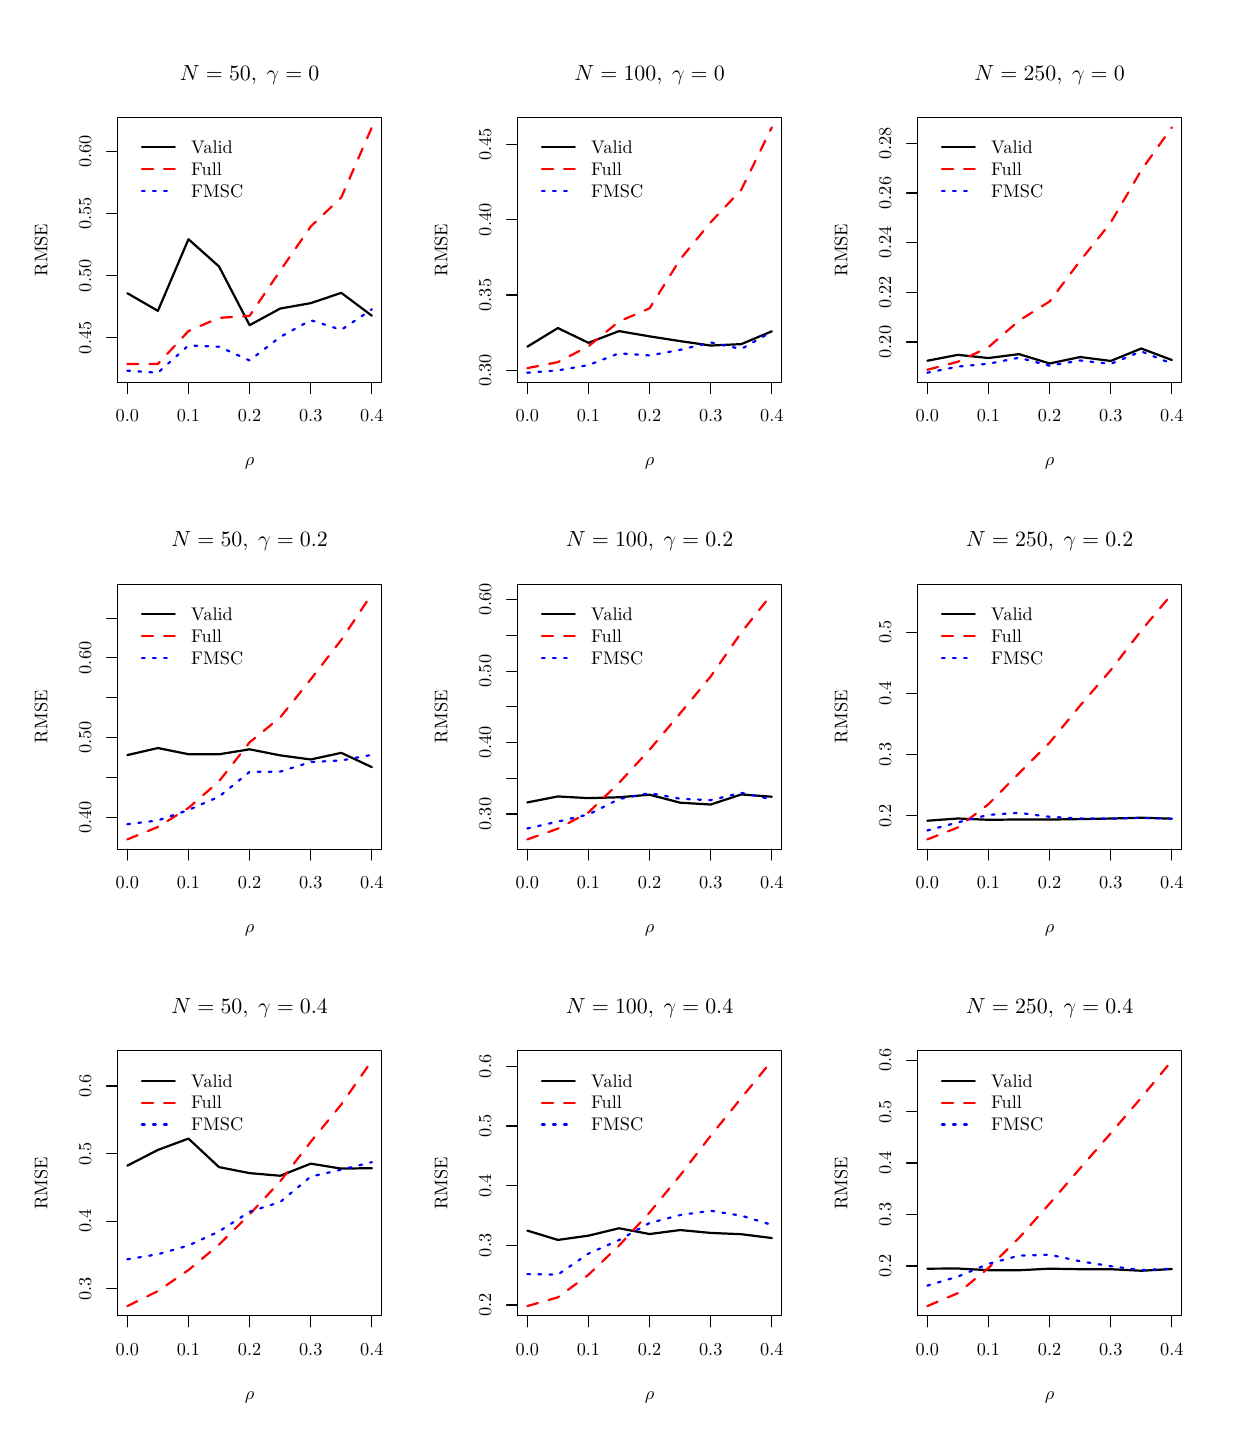
\begin{tikzpicture}[x=1pt,y=1pt]
\definecolor[named]{fillColor}{rgb}{1.00,1.00,1.00}
\path[use as bounding box,fill=fillColor,fill opacity=0.00] (0,0) rectangle (433.62,505.89);
\begin{scope}
\path[clip] ( 32.47,377.65) rectangle (127.91,473.42);
\definecolor[named]{drawColor}{rgb}{0.00,0.00,0.00}

\path[draw=drawColor,line width= 0.8pt,line join=round,line cap=round] ( 36.01,409.93) --
	( 47.05,403.55) --
	( 58.10,429.44) --
	( 69.14,419.60) --
	( 80.19,398.38) --
	( 91.24,404.39) --
	(102.28,406.34) --
	(113.33,410.06) --
	(124.37,401.80);
\end{scope}
\begin{scope}
\path[clip] (  0.00,  0.00) rectangle (433.62,505.89);
\definecolor[named]{drawColor}{rgb}{0.00,0.00,0.00}

\path[draw=drawColor,line width= 0.4pt,line join=round,line cap=round] ( 36.01,377.65) -- (124.37,377.65);

\path[draw=drawColor,line width= 0.4pt,line join=round,line cap=round] ( 36.01,377.65) -- ( 36.01,373.69);

\path[draw=drawColor,line width= 0.4pt,line join=round,line cap=round] ( 58.10,377.65) -- ( 58.10,373.69);

\path[draw=drawColor,line width= 0.4pt,line join=round,line cap=round] ( 80.19,377.65) -- ( 80.19,373.69);

\path[draw=drawColor,line width= 0.4pt,line join=round,line cap=round] (102.28,377.65) -- (102.28,373.69);

\path[draw=drawColor,line width= 0.4pt,line join=round,line cap=round] (124.37,377.65) -- (124.37,373.69);

\node[text=drawColor,anchor=base,inner sep=0pt, outer sep=0pt, scale=  0.66] at ( 36.01,363.40) {0.0};

\node[text=drawColor,anchor=base,inner sep=0pt, outer sep=0pt, scale=  0.66] at ( 58.10,363.40) {0.1};

\node[text=drawColor,anchor=base,inner sep=0pt, outer sep=0pt, scale=  0.66] at ( 80.19,363.40) {0.2};

\node[text=drawColor,anchor=base,inner sep=0pt, outer sep=0pt, scale=  0.66] at (102.28,363.40) {0.3};

\node[text=drawColor,anchor=base,inner sep=0pt, outer sep=0pt, scale=  0.66] at (124.37,363.40) {0.4};

\path[draw=drawColor,line width= 0.4pt,line join=round,line cap=round] ( 32.47,393.82) -- ( 32.47,461.07);

\path[draw=drawColor,line width= 0.4pt,line join=round,line cap=round] ( 32.47,393.82) -- ( 28.51,393.82);

\path[draw=drawColor,line width= 0.4pt,line join=round,line cap=round] ( 32.47,416.24) -- ( 28.51,416.24);

\path[draw=drawColor,line width= 0.4pt,line join=round,line cap=round] ( 32.47,438.65) -- ( 28.51,438.65);

\path[draw=drawColor,line width= 0.4pt,line join=round,line cap=round] ( 32.47,461.07) -- ( 28.51,461.07);

\node[text=drawColor,rotate= 90.00,anchor=base,inner sep=0pt, outer sep=0pt, scale=  0.66] at ( 22.97,393.82) {0.45};

\node[text=drawColor,rotate= 90.00,anchor=base,inner sep=0pt, outer sep=0pt, scale=  0.66] at ( 22.97,416.24) {0.50};

\node[text=drawColor,rotate= 90.00,anchor=base,inner sep=0pt, outer sep=0pt, scale=  0.66] at ( 22.97,438.65) {0.55};

\node[text=drawColor,rotate= 90.00,anchor=base,inner sep=0pt, outer sep=0pt, scale=  0.66] at ( 22.97,461.07) {0.60};

\path[draw=drawColor,line width= 0.4pt,line join=round,line cap=round] ( 32.47,377.65) --
	(127.91,377.65) --
	(127.91,473.42) --
	( 32.47,473.42) --
	( 32.47,377.65);
\end{scope}
\begin{scope}
\path[clip] (  0.00,337.26) rectangle (144.54,505.89);
\definecolor[named]{drawColor}{rgb}{0.00,0.00,0.00}

\node[text=drawColor,anchor=base,inner sep=0pt, outer sep=0pt, scale=  0.79] at ( 80.19,486.92) {\bfseries $N=50, \;\gamma=0$};

\node[text=drawColor,anchor=base,inner sep=0pt, outer sep=0pt, scale=  0.66] at ( 80.19,347.56) {$\rho$};

\node[text=drawColor,rotate= 90.00,anchor=base,inner sep=0pt, outer sep=0pt, scale=  0.66] at (  7.13,425.53) {RMSE};
\end{scope}
\begin{scope}
\path[clip] ( 32.47,377.65) rectangle (127.91,473.42);
\definecolor[named]{drawColor}{rgb}{1.00,0.00,0.00}

\path[draw=drawColor,line width= 0.8pt,dash pattern=on 4pt off 4pt ,line join=round,line cap=round] ( 36.01,384.36) --
	( 47.05,384.37) --
	( 58.10,396.26) --
	( 69.14,401.02) --
	( 80.19,401.76) --
	( 91.24,418.05) --
	(102.28,434.02) --
	(113.33,444.56) --
	(124.37,469.87);
\definecolor[named]{drawColor}{rgb}{0.00,0.00,1.00}

\path[draw=drawColor,line width= 0.8pt,dash pattern=on 1pt off 3pt ,line join=round,line cap=round] ( 36.01,381.95) --
	( 47.05,381.20) --
	( 58.10,391.05) --
	( 69.14,390.60) --
	( 80.19,385.63) --
	( 91.24,394.12) --
	(102.28,400.17) --
	(113.33,396.69) --
	(124.37,404.12);
\definecolor[named]{drawColor}{rgb}{0.00,0.00,0.00}

\path[draw=drawColor,line width= 0.8pt,line join=round,line cap=round] ( 41.28,462.63) -- ( 53.16,462.63);
\definecolor[named]{drawColor}{rgb}{1.00,0.00,0.00}

\path[draw=drawColor,line width= 0.8pt,dash pattern=on 4pt off 4pt ,line join=round,line cap=round] ( 41.28,454.71) -- ( 53.16,454.71);
\definecolor[named]{drawColor}{rgb}{0.00,0.00,1.00}

\path[draw=drawColor,line width= 0.8pt,dash pattern=on 1pt off 3pt ,line join=round,line cap=round] ( 41.28,446.79) -- ( 53.16,446.79);
\definecolor[named]{drawColor}{rgb}{0.00,0.00,0.00}

\node[text=drawColor,anchor=base west,inner sep=0pt, outer sep=0pt, scale=  0.66] at ( 59.10,460.35) {Valid};

\node[text=drawColor,anchor=base west,inner sep=0pt, outer sep=0pt, scale=  0.66] at ( 59.10,452.43) {Full};

\node[text=drawColor,anchor=base west,inner sep=0pt, outer sep=0pt, scale=  0.66] at ( 59.10,444.51) {FMSC};
\end{scope}
\begin{scope}
\path[clip] (177.01,377.65) rectangle (272.45,473.42);
\definecolor[named]{drawColor}{rgb}{0.00,0.00,0.00}

\path[draw=drawColor,line width= 0.8pt,line join=round,line cap=round] (180.55,390.61) --
	(191.59,397.34) --
	(202.64,392.01) --
	(213.68,396.24) --
	(224.73,394.34) --
	(235.78,392.62) --
	(246.82,391.02) --
	(257.87,391.54) --
	(268.91,396.17);
\end{scope}
\begin{scope}
\path[clip] (  0.00,  0.00) rectangle (433.62,505.89);
\definecolor[named]{drawColor}{rgb}{0.00,0.00,0.00}

\path[draw=drawColor,line width= 0.4pt,line join=round,line cap=round] (180.55,377.65) -- (268.91,377.65);

\path[draw=drawColor,line width= 0.4pt,line join=round,line cap=round] (180.55,377.65) -- (180.55,373.69);

\path[draw=drawColor,line width= 0.4pt,line join=round,line cap=round] (202.64,377.65) -- (202.64,373.69);

\path[draw=drawColor,line width= 0.4pt,line join=round,line cap=round] (224.73,377.65) -- (224.73,373.69);

\path[draw=drawColor,line width= 0.4pt,line join=round,line cap=round] (246.82,377.65) -- (246.82,373.69);

\path[draw=drawColor,line width= 0.4pt,line join=round,line cap=round] (268.91,377.65) -- (268.91,373.69);

\node[text=drawColor,anchor=base,inner sep=0pt, outer sep=0pt, scale=  0.66] at (180.55,363.40) {0.0};

\node[text=drawColor,anchor=base,inner sep=0pt, outer sep=0pt, scale=  0.66] at (202.64,363.40) {0.1};

\node[text=drawColor,anchor=base,inner sep=0pt, outer sep=0pt, scale=  0.66] at (224.73,363.40) {0.2};

\node[text=drawColor,anchor=base,inner sep=0pt, outer sep=0pt, scale=  0.66] at (246.82,363.40) {0.3};

\node[text=drawColor,anchor=base,inner sep=0pt, outer sep=0pt, scale=  0.66] at (268.91,363.40) {0.4};

\path[draw=drawColor,line width= 0.4pt,line join=round,line cap=round] (177.01,382.08) -- (177.01,463.66);

\path[draw=drawColor,line width= 0.4pt,line join=round,line cap=round] (177.01,382.08) -- (173.05,382.08);

\path[draw=drawColor,line width= 0.4pt,line join=round,line cap=round] (177.01,409.27) -- (173.05,409.27);

\path[draw=drawColor,line width= 0.4pt,line join=round,line cap=round] (177.01,436.47) -- (173.05,436.47);

\path[draw=drawColor,line width= 0.4pt,line join=round,line cap=round] (177.01,463.66) -- (173.05,463.66);

\node[text=drawColor,rotate= 90.00,anchor=base,inner sep=0pt, outer sep=0pt, scale=  0.66] at (167.51,382.08) {0.30};

\node[text=drawColor,rotate= 90.00,anchor=base,inner sep=0pt, outer sep=0pt, scale=  0.66] at (167.51,409.27) {0.35};

\node[text=drawColor,rotate= 90.00,anchor=base,inner sep=0pt, outer sep=0pt, scale=  0.66] at (167.51,436.47) {0.40};

\node[text=drawColor,rotate= 90.00,anchor=base,inner sep=0pt, outer sep=0pt, scale=  0.66] at (167.51,463.66) {0.45};

\path[draw=drawColor,line width= 0.4pt,line join=round,line cap=round] (177.01,377.65) --
	(272.45,377.65) --
	(272.45,473.42) --
	(177.01,473.42) --
	(177.01,377.65);
\end{scope}
\begin{scope}
\path[clip] (144.54,337.26) rectangle (289.08,505.89);
\definecolor[named]{drawColor}{rgb}{0.00,0.00,0.00}

\node[text=drawColor,anchor=base,inner sep=0pt, outer sep=0pt, scale=  0.79] at (224.73,486.92) {\bfseries $N=100, \;\gamma=0$};

\node[text=drawColor,anchor=base,inner sep=0pt, outer sep=0pt, scale=  0.66] at (224.73,347.56) {$\rho$};

\node[text=drawColor,rotate= 90.00,anchor=base,inner sep=0pt, outer sep=0pt, scale=  0.66] at (151.67,425.53) {RMSE};
\end{scope}
\begin{scope}
\path[clip] (177.01,377.65) rectangle (272.45,473.42);
\definecolor[named]{drawColor}{rgb}{1.00,0.00,0.00}

\path[draw=drawColor,line width= 0.8pt,dash pattern=on 4pt off 4pt ,line join=round,line cap=round] (180.55,382.86) --
	(191.59,385.03) --
	(202.64,390.76) --
	(213.68,399.73) --
	(224.73,404.46) --
	(235.78,422.18) --
	(246.82,435.60) --
	(257.87,447.35) --
	(268.91,469.87);
\definecolor[named]{drawColor}{rgb}{0.00,0.00,1.00}

\path[draw=drawColor,line width= 0.8pt,dash pattern=on 1pt off 3pt ,line join=round,line cap=round] (180.55,381.20) --
	(191.59,382.04) --
	(202.64,383.96) --
	(213.68,388.21) --
	(224.73,387.44) --
	(235.78,389.48) --
	(246.82,392.15) --
	(257.87,389.77) --
	(268.91,396.06);
\definecolor[named]{drawColor}{rgb}{0.00,0.00,0.00}

\path[draw=drawColor,line width= 0.8pt,line join=round,line cap=round] (185.82,462.63) -- (197.70,462.63);
\definecolor[named]{drawColor}{rgb}{1.00,0.00,0.00}

\path[draw=drawColor,line width= 0.8pt,dash pattern=on 4pt off 4pt ,line join=round,line cap=round] (185.82,454.71) -- (197.70,454.71);
\definecolor[named]{drawColor}{rgb}{0.00,0.00,1.00}

\path[draw=drawColor,line width= 0.8pt,dash pattern=on 1pt off 3pt ,line join=round,line cap=round] (185.82,446.79) -- (197.70,446.79);
\definecolor[named]{drawColor}{rgb}{0.00,0.00,0.00}

\node[text=drawColor,anchor=base west,inner sep=0pt, outer sep=0pt, scale=  0.66] at (203.64,460.35) {Valid};

\node[text=drawColor,anchor=base west,inner sep=0pt, outer sep=0pt, scale=  0.66] at (203.64,452.43) {Full};

\node[text=drawColor,anchor=base west,inner sep=0pt, outer sep=0pt, scale=  0.66] at (203.64,444.51) {FMSC};
\end{scope}
\begin{scope}
\path[clip] (321.55,377.65) rectangle (416.99,473.42);
\definecolor[named]{drawColor}{rgb}{0.00,0.00,0.00}

\path[draw=drawColor,line width= 0.8pt,line join=round,line cap=round] (325.09,385.53) --
	(336.13,387.66) --
	(347.18,386.51) --
	(358.22,387.92) --
	(369.27,384.54) --
	(380.32,386.87) --
	(391.36,385.46) --
	(402.41,389.95) --
	(413.45,385.80);
\end{scope}
\begin{scope}
\path[clip] (  0.00,  0.00) rectangle (433.62,505.89);
\definecolor[named]{drawColor}{rgb}{0.00,0.00,0.00}

\path[draw=drawColor,line width= 0.4pt,line join=round,line cap=round] (325.09,377.65) -- (413.45,377.65);

\path[draw=drawColor,line width= 0.4pt,line join=round,line cap=round] (325.09,377.65) -- (325.09,373.69);

\path[draw=drawColor,line width= 0.4pt,line join=round,line cap=round] (347.18,377.65) -- (347.18,373.69);

\path[draw=drawColor,line width= 0.4pt,line join=round,line cap=round] (369.27,377.65) -- (369.27,373.69);

\path[draw=drawColor,line width= 0.4pt,line join=round,line cap=round] (391.36,377.65) -- (391.36,373.69);

\path[draw=drawColor,line width= 0.4pt,line join=round,line cap=round] (413.45,377.65) -- (413.45,373.69);

\node[text=drawColor,anchor=base,inner sep=0pt, outer sep=0pt, scale=  0.66] at (325.09,363.40) {0.0};

\node[text=drawColor,anchor=base,inner sep=0pt, outer sep=0pt, scale=  0.66] at (347.18,363.40) {0.1};

\node[text=drawColor,anchor=base,inner sep=0pt, outer sep=0pt, scale=  0.66] at (369.27,363.40) {0.2};

\node[text=drawColor,anchor=base,inner sep=0pt, outer sep=0pt, scale=  0.66] at (391.36,363.40) {0.3};

\node[text=drawColor,anchor=base,inner sep=0pt, outer sep=0pt, scale=  0.66] at (413.45,363.40) {0.4};

\path[draw=drawColor,line width= 0.4pt,line join=round,line cap=round] (321.55,392.31) -- (321.55,464.09);

\path[draw=drawColor,line width= 0.4pt,line join=round,line cap=round] (321.55,392.31) -- (317.59,392.31);

\path[draw=drawColor,line width= 0.4pt,line join=round,line cap=round] (321.55,410.26) -- (317.59,410.26);

\path[draw=drawColor,line width= 0.4pt,line join=round,line cap=round] (321.55,428.20) -- (317.59,428.20);

\path[draw=drawColor,line width= 0.4pt,line join=round,line cap=round] (321.55,446.14) -- (317.59,446.14);

\path[draw=drawColor,line width= 0.4pt,line join=round,line cap=round] (321.55,464.09) -- (317.59,464.09);

\node[text=drawColor,rotate= 90.00,anchor=base,inner sep=0pt, outer sep=0pt, scale=  0.66] at (312.05,392.31) {0.20};

\node[text=drawColor,rotate= 90.00,anchor=base,inner sep=0pt, outer sep=0pt, scale=  0.66] at (312.05,410.26) {0.22};

\node[text=drawColor,rotate= 90.00,anchor=base,inner sep=0pt, outer sep=0pt, scale=  0.66] at (312.05,428.20) {0.24};

\node[text=drawColor,rotate= 90.00,anchor=base,inner sep=0pt, outer sep=0pt, scale=  0.66] at (312.05,446.14) {0.26};

\node[text=drawColor,rotate= 90.00,anchor=base,inner sep=0pt, outer sep=0pt, scale=  0.66] at (312.05,464.09) {0.28};

\path[draw=drawColor,line width= 0.4pt,line join=round,line cap=round] (321.55,377.65) --
	(416.99,377.65) --
	(416.99,473.42) --
	(321.55,473.42) --
	(321.55,377.65);
\end{scope}
\begin{scope}
\path[clip] (289.08,337.26) rectangle (433.62,505.89);
\definecolor[named]{drawColor}{rgb}{0.00,0.00,0.00}

\node[text=drawColor,anchor=base,inner sep=0pt, outer sep=0pt, scale=  0.79] at (369.27,486.92) {\bfseries $N=250, \;\gamma=0$};

\node[text=drawColor,anchor=base,inner sep=0pt, outer sep=0pt, scale=  0.66] at (369.27,347.56) {$\rho$};

\node[text=drawColor,rotate= 90.00,anchor=base,inner sep=0pt, outer sep=0pt, scale=  0.66] at (296.21,425.53) {RMSE};
\end{scope}
\begin{scope}
\path[clip] (321.55,377.65) rectangle (416.99,473.42);
\definecolor[named]{drawColor}{rgb}{1.00,0.00,0.00}

\path[draw=drawColor,line width= 0.8pt,dash pattern=on 4pt off 4pt ,line join=round,line cap=round] (325.09,382.28) --
	(336.13,385.16) --
	(347.18,390.42) --
	(358.22,400.03) --
	(369.27,406.95) --
	(380.32,421.67) --
	(391.36,435.45) --
	(402.41,454.40) --
	(413.45,469.87);
\definecolor[named]{drawColor}{rgb}{0.00,0.00,1.00}

\path[draw=drawColor,line width= 0.8pt,dash pattern=on 1pt off 3pt ,line join=round,line cap=round] (325.09,381.20) --
	(336.13,383.41) --
	(347.18,384.45) --
	(358.22,386.62) --
	(369.27,383.73) --
	(380.32,385.63) --
	(391.36,384.38) --
	(402.41,388.92) --
	(413.45,384.46);
\definecolor[named]{drawColor}{rgb}{0.00,0.00,0.00}

\path[draw=drawColor,line width= 0.8pt,line join=round,line cap=round] (330.36,462.63) -- (342.24,462.63);
\definecolor[named]{drawColor}{rgb}{1.00,0.00,0.00}

\path[draw=drawColor,line width= 0.8pt,dash pattern=on 4pt off 4pt ,line join=round,line cap=round] (330.36,454.71) -- (342.24,454.71);
\definecolor[named]{drawColor}{rgb}{0.00,0.00,1.00}

\path[draw=drawColor,line width= 0.8pt,dash pattern=on 1pt off 3pt ,line join=round,line cap=round] (330.36,446.79) -- (342.24,446.79);
\definecolor[named]{drawColor}{rgb}{0.00,0.00,0.00}

\node[text=drawColor,anchor=base west,inner sep=0pt, outer sep=0pt, scale=  0.66] at (348.18,460.35) {Valid};

\node[text=drawColor,anchor=base west,inner sep=0pt, outer sep=0pt, scale=  0.66] at (348.18,452.43) {Full};

\node[text=drawColor,anchor=base west,inner sep=0pt, outer sep=0pt, scale=  0.66] at (348.18,444.51) {FMSC};
\end{scope}
\begin{scope}
\path[clip] ( 32.47,209.02) rectangle (127.91,304.79);
\definecolor[named]{drawColor}{rgb}{0.00,0.00,0.00}

\path[draw=drawColor,line width= 0.8pt,line join=round,line cap=round] ( 36.01,243.04) --
	( 47.05,245.58) --
	( 58.10,243.36) --
	( 69.14,243.32) --
	( 80.19,245.12) --
	( 91.24,242.94) --
	(102.28,241.45) --
	(113.33,243.85) --
	(124.37,238.68);
\end{scope}
\begin{scope}
\path[clip] (  0.00,  0.00) rectangle (433.62,505.89);
\definecolor[named]{drawColor}{rgb}{0.00,0.00,0.00}

\path[draw=drawColor,line width= 0.4pt,line join=round,line cap=round] ( 36.01,209.02) -- (124.37,209.02);

\path[draw=drawColor,line width= 0.4pt,line join=round,line cap=round] ( 36.01,209.02) -- ( 36.01,205.06);

\path[draw=drawColor,line width= 0.4pt,line join=round,line cap=round] ( 58.10,209.02) -- ( 58.10,205.06);

\path[draw=drawColor,line width= 0.4pt,line join=round,line cap=round] ( 80.19,209.02) -- ( 80.19,205.06);

\path[draw=drawColor,line width= 0.4pt,line join=round,line cap=round] (102.28,209.02) -- (102.28,205.06);

\path[draw=drawColor,line width= 0.4pt,line join=round,line cap=round] (124.37,209.02) -- (124.37,205.06);

\node[text=drawColor,anchor=base,inner sep=0pt, outer sep=0pt, scale=  0.66] at ( 36.01,194.77) {0.0};

\node[text=drawColor,anchor=base,inner sep=0pt, outer sep=0pt, scale=  0.66] at ( 58.10,194.77) {0.1};

\node[text=drawColor,anchor=base,inner sep=0pt, outer sep=0pt, scale=  0.66] at ( 80.19,194.77) {0.2};

\node[text=drawColor,anchor=base,inner sep=0pt, outer sep=0pt, scale=  0.66] at (102.28,194.77) {0.3};

\node[text=drawColor,anchor=base,inner sep=0pt, outer sep=0pt, scale=  0.66] at (124.37,194.77) {0.4};

\path[draw=drawColor,line width= 0.4pt,line join=round,line cap=round] ( 32.47,220.60) -- ( 32.47,292.53);

\path[draw=drawColor,line width= 0.4pt,line join=round,line cap=round] ( 32.47,220.60) -- ( 28.51,220.60);

\path[draw=drawColor,line width= 0.4pt,line join=round,line cap=round] ( 32.47,234.99) -- ( 28.51,234.99);

\path[draw=drawColor,line width= 0.4pt,line join=round,line cap=round] ( 32.47,249.37) -- ( 28.51,249.37);

\path[draw=drawColor,line width= 0.4pt,line join=round,line cap=round] ( 32.47,263.76) -- ( 28.51,263.76);

\path[draw=drawColor,line width= 0.4pt,line join=round,line cap=round] ( 32.47,278.14) -- ( 28.51,278.14);

\path[draw=drawColor,line width= 0.4pt,line join=round,line cap=round] ( 32.47,292.53) -- ( 28.51,292.53);

\node[text=drawColor,rotate= 90.00,anchor=base,inner sep=0pt, outer sep=0pt, scale=  0.66] at ( 22.97,220.60) {0.40};

\node[text=drawColor,rotate= 90.00,anchor=base,inner sep=0pt, outer sep=0pt, scale=  0.66] at ( 22.97,249.37) {0.50};

\node[text=drawColor,rotate= 90.00,anchor=base,inner sep=0pt, outer sep=0pt, scale=  0.66] at ( 22.97,278.14) {0.60};

\path[draw=drawColor,line width= 0.4pt,line join=round,line cap=round] ( 32.47,209.02) --
	(127.91,209.02) --
	(127.91,304.79) --
	( 32.47,304.79) --
	( 32.47,209.02);
\end{scope}
\begin{scope}
\path[clip] (  0.00,168.63) rectangle (144.54,337.26);
\definecolor[named]{drawColor}{rgb}{0.00,0.00,0.00}

\node[text=drawColor,anchor=base,inner sep=0pt, outer sep=0pt, scale=  0.79] at ( 80.19,318.29) {\bfseries $N=50, \;\gamma=0.2$};

\node[text=drawColor,anchor=base,inner sep=0pt, outer sep=0pt, scale=  0.66] at ( 80.19,178.93) {$\rho$};

\node[text=drawColor,rotate= 90.00,anchor=base,inner sep=0pt, outer sep=0pt, scale=  0.66] at (  7.13,256.90) {RMSE};
\end{scope}
\begin{scope}
\path[clip] ( 32.47,209.02) rectangle (127.91,304.79);
\definecolor[named]{drawColor}{rgb}{1.00,0.00,0.00}

\path[draw=drawColor,line width= 0.8pt,dash pattern=on 4pt off 4pt ,line join=round,line cap=round] ( 36.01,212.57) --
	( 47.05,217.05) --
	( 58.10,223.95) --
	( 69.14,233.55) --
	( 80.19,247.63) --
	( 91.24,256.64) --
	(102.28,270.40) --
	(113.33,284.68) --
	(124.37,301.24);
\definecolor[named]{drawColor}{rgb}{0.00,0.00,1.00}

\path[draw=drawColor,line width= 0.8pt,dash pattern=on 1pt off 3pt ,line join=round,line cap=round] ( 36.01,218.06) --
	( 47.05,219.41) --
	( 58.10,223.20) --
	( 69.14,228.01) --
	( 80.19,236.97) --
	( 91.24,237.06) --
	(102.28,240.53) --
	(113.33,241.09) --
	(124.37,243.13);
\definecolor[named]{drawColor}{rgb}{0.00,0.00,0.00}

\path[draw=drawColor,line width= 0.8pt,line join=round,line cap=round] ( 41.28,294.00) -- ( 53.16,294.00);
\definecolor[named]{drawColor}{rgb}{1.00,0.00,0.00}

\path[draw=drawColor,line width= 0.8pt,dash pattern=on 4pt off 4pt ,line join=round,line cap=round] ( 41.28,286.08) -- ( 53.16,286.08);
\definecolor[named]{drawColor}{rgb}{0.00,0.00,1.00}

\path[draw=drawColor,line width= 0.8pt,dash pattern=on 1pt off 3pt ,line join=round,line cap=round] ( 41.28,278.16) -- ( 53.16,278.16);
\definecolor[named]{drawColor}{rgb}{0.00,0.00,0.00}

\node[text=drawColor,anchor=base west,inner sep=0pt, outer sep=0pt, scale=  0.66] at ( 59.10,291.72) {Valid};

\node[text=drawColor,anchor=base west,inner sep=0pt, outer sep=0pt, scale=  0.66] at ( 59.10,283.80) {Full};

\node[text=drawColor,anchor=base west,inner sep=0pt, outer sep=0pt, scale=  0.66] at ( 59.10,275.88) {FMSC};
\end{scope}
\begin{scope}
\path[clip] (177.01,209.02) rectangle (272.45,304.79);
\definecolor[named]{drawColor}{rgb}{0.00,0.00,0.00}

\path[draw=drawColor,line width= 0.8pt,line join=round,line cap=round] (180.55,225.93) --
	(191.59,228.09) --
	(202.64,227.48) --
	(213.68,227.79) --
	(224.73,228.72) --
	(235.78,225.83) --
	(246.82,225.17) --
	(257.87,228.81) --
	(268.91,227.99);
\end{scope}
\begin{scope}
\path[clip] (  0.00,  0.00) rectangle (433.62,505.89);
\definecolor[named]{drawColor}{rgb}{0.00,0.00,0.00}

\path[draw=drawColor,line width= 0.4pt,line join=round,line cap=round] (180.55,209.02) -- (268.91,209.02);

\path[draw=drawColor,line width= 0.4pt,line join=round,line cap=round] (180.55,209.02) -- (180.55,205.06);

\path[draw=drawColor,line width= 0.4pt,line join=round,line cap=round] (202.64,209.02) -- (202.64,205.06);

\path[draw=drawColor,line width= 0.4pt,line join=round,line cap=round] (224.73,209.02) -- (224.73,205.06);

\path[draw=drawColor,line width= 0.4pt,line join=round,line cap=round] (246.82,209.02) -- (246.82,205.06);

\path[draw=drawColor,line width= 0.4pt,line join=round,line cap=round] (268.91,209.02) -- (268.91,205.06);

\node[text=drawColor,anchor=base,inner sep=0pt, outer sep=0pt, scale=  0.66] at (180.55,194.77) {0.0};

\node[text=drawColor,anchor=base,inner sep=0pt, outer sep=0pt, scale=  0.66] at (202.64,194.77) {0.1};

\node[text=drawColor,anchor=base,inner sep=0pt, outer sep=0pt, scale=  0.66] at (224.73,194.77) {0.2};

\node[text=drawColor,anchor=base,inner sep=0pt, outer sep=0pt, scale=  0.66] at (246.82,194.77) {0.3};

\node[text=drawColor,anchor=base,inner sep=0pt, outer sep=0pt, scale=  0.66] at (268.91,194.77) {0.4};

\path[draw=drawColor,line width= 0.4pt,line join=round,line cap=round] (177.01,221.73) -- (177.01,299.24);

\path[draw=drawColor,line width= 0.4pt,line join=round,line cap=round] (177.01,221.73) -- (173.05,221.73);

\path[draw=drawColor,line width= 0.4pt,line join=round,line cap=round] (177.01,234.65) -- (173.05,234.65);

\path[draw=drawColor,line width= 0.4pt,line join=round,line cap=round] (177.01,247.56) -- (173.05,247.56);

\path[draw=drawColor,line width= 0.4pt,line join=round,line cap=round] (177.01,260.48) -- (173.05,260.48);

\path[draw=drawColor,line width= 0.4pt,line join=round,line cap=round] (177.01,273.40) -- (173.05,273.40);

\path[draw=drawColor,line width= 0.4pt,line join=round,line cap=round] (177.01,286.32) -- (173.05,286.32);

\path[draw=drawColor,line width= 0.4pt,line join=round,line cap=round] (177.01,299.24) -- (173.05,299.24);

\node[text=drawColor,rotate= 90.00,anchor=base,inner sep=0pt, outer sep=0pt, scale=  0.66] at (167.51,221.73) {0.30};

\node[text=drawColor,rotate= 90.00,anchor=base,inner sep=0pt, outer sep=0pt, scale=  0.66] at (167.51,247.56) {0.40};

\node[text=drawColor,rotate= 90.00,anchor=base,inner sep=0pt, outer sep=0pt, scale=  0.66] at (167.51,273.40) {0.50};

\node[text=drawColor,rotate= 90.00,anchor=base,inner sep=0pt, outer sep=0pt, scale=  0.66] at (167.51,299.24) {0.60};

\path[draw=drawColor,line width= 0.4pt,line join=round,line cap=round] (177.01,209.02) --
	(272.45,209.02) --
	(272.45,304.79) --
	(177.01,304.79) --
	(177.01,209.02);
\end{scope}
\begin{scope}
\path[clip] (144.54,168.63) rectangle (289.08,337.26);
\definecolor[named]{drawColor}{rgb}{0.00,0.00,0.00}

\node[text=drawColor,anchor=base,inner sep=0pt, outer sep=0pt, scale=  0.79] at (224.73,318.29) {\bfseries $N=100, \;\gamma=0.2$};

\node[text=drawColor,anchor=base,inner sep=0pt, outer sep=0pt, scale=  0.66] at (224.73,178.93) {$\rho$};

\node[text=drawColor,rotate= 90.00,anchor=base,inner sep=0pt, outer sep=0pt, scale=  0.66] at (151.67,256.90) {RMSE};
\end{scope}
\begin{scope}
\path[clip] (177.01,209.02) rectangle (272.45,304.79);
\definecolor[named]{drawColor}{rgb}{1.00,0.00,0.00}

\path[draw=drawColor,line width= 0.8pt,dash pattern=on 4pt off 4pt ,line join=round,line cap=round] (180.55,212.57) --
	(191.59,216.45) --
	(202.64,222.30) --
	(213.68,232.98) --
	(224.73,244.97) --
	(235.78,258.13) --
	(246.82,271.45) --
	(257.87,287.33) --
	(268.91,301.24);
\definecolor[named]{drawColor}{rgb}{0.00,0.00,1.00}

\path[draw=drawColor,line width= 0.8pt,dash pattern=on 1pt off 3pt ,line join=round,line cap=round] (180.55,216.53) --
	(191.59,219.00) --
	(202.64,221.59) --
	(213.68,227.13) --
	(224.73,229.31) --
	(235.78,227.25) --
	(246.82,226.75) --
	(257.87,229.41) --
	(268.91,227.02);
\definecolor[named]{drawColor}{rgb}{0.00,0.00,0.00}

\path[draw=drawColor,line width= 0.8pt,line join=round,line cap=round] (185.82,294.00) -- (197.70,294.00);
\definecolor[named]{drawColor}{rgb}{1.00,0.00,0.00}

\path[draw=drawColor,line width= 0.8pt,dash pattern=on 4pt off 4pt ,line join=round,line cap=round] (185.82,286.08) -- (197.70,286.08);
\definecolor[named]{drawColor}{rgb}{0.00,0.00,1.00}

\path[draw=drawColor,line width= 0.8pt,dash pattern=on 1pt off 3pt ,line join=round,line cap=round] (185.82,278.16) -- (197.70,278.16);
\definecolor[named]{drawColor}{rgb}{0.00,0.00,0.00}

\node[text=drawColor,anchor=base west,inner sep=0pt, outer sep=0pt, scale=  0.66] at (203.64,291.72) {Valid};

\node[text=drawColor,anchor=base west,inner sep=0pt, outer sep=0pt, scale=  0.66] at (203.64,283.80) {Full};

\node[text=drawColor,anchor=base west,inner sep=0pt, outer sep=0pt, scale=  0.66] at (203.64,275.88) {FMSC};
\end{scope}
\begin{scope}
\path[clip] (321.55,209.02) rectangle (416.99,304.79);
\definecolor[named]{drawColor}{rgb}{0.00,0.00,0.00}

\path[draw=drawColor,line width= 0.8pt,line join=round,line cap=round] (325.09,219.32) --
	(336.13,220.12) --
	(347.18,219.66) --
	(358.22,219.76) --
	(369.27,219.74) --
	(380.32,219.91) --
	(391.36,220.10) --
	(402.41,220.40) --
	(413.45,220.05);
\end{scope}
\begin{scope}
\path[clip] (  0.00,  0.00) rectangle (433.62,505.89);
\definecolor[named]{drawColor}{rgb}{0.00,0.00,0.00}

\path[draw=drawColor,line width= 0.4pt,line join=round,line cap=round] (325.09,209.02) -- (413.45,209.02);

\path[draw=drawColor,line width= 0.4pt,line join=round,line cap=round] (325.09,209.02) -- (325.09,205.06);

\path[draw=drawColor,line width= 0.4pt,line join=round,line cap=round] (347.18,209.02) -- (347.18,205.06);

\path[draw=drawColor,line width= 0.4pt,line join=round,line cap=round] (369.27,209.02) -- (369.27,205.06);

\path[draw=drawColor,line width= 0.4pt,line join=round,line cap=round] (391.36,209.02) -- (391.36,205.06);

\path[draw=drawColor,line width= 0.4pt,line join=round,line cap=round] (413.45,209.02) -- (413.45,205.06);

\node[text=drawColor,anchor=base,inner sep=0pt, outer sep=0pt, scale=  0.66] at (325.09,194.77) {0.0};

\node[text=drawColor,anchor=base,inner sep=0pt, outer sep=0pt, scale=  0.66] at (347.18,194.77) {0.1};

\node[text=drawColor,anchor=base,inner sep=0pt, outer sep=0pt, scale=  0.66] at (369.27,194.77) {0.2};

\node[text=drawColor,anchor=base,inner sep=0pt, outer sep=0pt, scale=  0.66] at (391.36,194.77) {0.3};

\node[text=drawColor,anchor=base,inner sep=0pt, outer sep=0pt, scale=  0.66] at (413.45,194.77) {0.4};

\path[draw=drawColor,line width= 0.4pt,line join=round,line cap=round] (321.55,221.16) -- (321.55,287.40);

\path[draw=drawColor,line width= 0.4pt,line join=round,line cap=round] (321.55,221.16) -- (317.59,221.16);

\path[draw=drawColor,line width= 0.4pt,line join=round,line cap=round] (321.55,243.24) -- (317.59,243.24);

\path[draw=drawColor,line width= 0.4pt,line join=round,line cap=round] (321.55,265.32) -- (317.59,265.32);

\path[draw=drawColor,line width= 0.4pt,line join=round,line cap=round] (321.55,287.40) -- (317.59,287.40);

\node[text=drawColor,rotate= 90.00,anchor=base,inner sep=0pt, outer sep=0pt, scale=  0.66] at (312.05,221.16) {0.2};

\node[text=drawColor,rotate= 90.00,anchor=base,inner sep=0pt, outer sep=0pt, scale=  0.66] at (312.05,243.24) {0.3};

\node[text=drawColor,rotate= 90.00,anchor=base,inner sep=0pt, outer sep=0pt, scale=  0.66] at (312.05,265.32) {0.4};

\node[text=drawColor,rotate= 90.00,anchor=base,inner sep=0pt, outer sep=0pt, scale=  0.66] at (312.05,287.40) {0.5};

\path[draw=drawColor,line width= 0.4pt,line join=round,line cap=round] (321.55,209.02) --
	(416.99,209.02) --
	(416.99,304.79) --
	(321.55,304.79) --
	(321.55,209.02);
\end{scope}
\begin{scope}
\path[clip] (289.08,168.63) rectangle (433.62,337.26);
\definecolor[named]{drawColor}{rgb}{0.00,0.00,0.00}

\node[text=drawColor,anchor=base,inner sep=0pt, outer sep=0pt, scale=  0.79] at (369.27,318.29) {\bfseries $N=250, \;\gamma=0.2$};

\node[text=drawColor,anchor=base,inner sep=0pt, outer sep=0pt, scale=  0.66] at (369.27,178.93) {$\rho$};

\node[text=drawColor,rotate= 90.00,anchor=base,inner sep=0pt, outer sep=0pt, scale=  0.66] at (296.21,256.90) {RMSE};
\end{scope}
\begin{scope}
\path[clip] (321.55,209.02) rectangle (416.99,304.79);
\definecolor[named]{drawColor}{rgb}{1.00,0.00,0.00}

\path[draw=drawColor,line width= 0.8pt,dash pattern=on 4pt off 4pt ,line join=round,line cap=round] (325.09,212.57) --
	(336.13,216.87) --
	(347.18,225.30) --
	(358.22,236.49) --
	(369.27,247.51) --
	(380.32,260.95) --
	(391.36,273.74) --
	(402.41,288.06) --
	(413.45,301.24);
\definecolor[named]{drawColor}{rgb}{0.00,0.00,1.00}

\path[draw=drawColor,line width= 0.8pt,dash pattern=on 1pt off 3pt ,line join=round,line cap=round] (325.09,215.79) --
	(336.13,218.72) --
	(347.18,221.43) --
	(358.22,222.17) --
	(369.27,220.73) --
	(380.32,220.11) --
	(391.36,220.09) --
	(402.41,220.38) --
	(413.45,220.05);
\definecolor[named]{drawColor}{rgb}{0.00,0.00,0.00}

\path[draw=drawColor,line width= 0.8pt,line join=round,line cap=round] (330.36,294.00) -- (342.24,294.00);
\definecolor[named]{drawColor}{rgb}{1.00,0.00,0.00}

\path[draw=drawColor,line width= 0.8pt,dash pattern=on 4pt off 4pt ,line join=round,line cap=round] (330.36,286.08) -- (342.24,286.08);
\definecolor[named]{drawColor}{rgb}{0.00,0.00,1.00}

\path[draw=drawColor,line width= 0.8pt,dash pattern=on 1pt off 3pt ,line join=round,line cap=round] (330.36,278.16) -- (342.24,278.16);
\definecolor[named]{drawColor}{rgb}{0.00,0.00,0.00}

\node[text=drawColor,anchor=base west,inner sep=0pt, outer sep=0pt, scale=  0.66] at (348.18,291.72) {Valid};

\node[text=drawColor,anchor=base west,inner sep=0pt, outer sep=0pt, scale=  0.66] at (348.18,283.80) {Full};

\node[text=drawColor,anchor=base west,inner sep=0pt, outer sep=0pt, scale=  0.66] at (348.18,275.88) {FMSC};
\end{scope}
\begin{scope}
\path[clip] ( 32.47, 40.39) rectangle (127.91,136.16);
\definecolor[named]{drawColor}{rgb}{0.00,0.00,0.00}

\path[draw=drawColor,line width= 0.8pt,line join=round,line cap=round] ( 36.01, 94.67) --
	( 47.05,100.36) --
	( 58.10,104.46) --
	( 69.14, 94.15) --
	( 80.19, 91.98) --
	( 91.24, 91.03) --
	(102.28, 95.40) --
	(113.33, 93.61) --
	(124.37, 93.77);
\end{scope}
\begin{scope}
\path[clip] (  0.00,  0.00) rectangle (433.62,505.89);
\definecolor[named]{drawColor}{rgb}{0.00,0.00,0.00}

\path[draw=drawColor,line width= 0.4pt,line join=round,line cap=round] ( 36.01, 40.39) -- (124.37, 40.39);

\path[draw=drawColor,line width= 0.4pt,line join=round,line cap=round] ( 36.01, 40.39) -- ( 36.01, 36.43);

\path[draw=drawColor,line width= 0.4pt,line join=round,line cap=round] ( 58.10, 40.39) -- ( 58.10, 36.43);

\path[draw=drawColor,line width= 0.4pt,line join=round,line cap=round] ( 80.19, 40.39) -- ( 80.19, 36.43);

\path[draw=drawColor,line width= 0.4pt,line join=round,line cap=round] (102.28, 40.39) -- (102.28, 36.43);

\path[draw=drawColor,line width= 0.4pt,line join=round,line cap=round] (124.37, 40.39) -- (124.37, 36.43);

\node[text=drawColor,anchor=base,inner sep=0pt, outer sep=0pt, scale=  0.66] at ( 36.01, 26.14) {0.0};

\node[text=drawColor,anchor=base,inner sep=0pt, outer sep=0pt, scale=  0.66] at ( 58.10, 26.14) {0.1};

\node[text=drawColor,anchor=base,inner sep=0pt, outer sep=0pt, scale=  0.66] at ( 80.19, 26.14) {0.2};

\node[text=drawColor,anchor=base,inner sep=0pt, outer sep=0pt, scale=  0.66] at (102.28, 26.14) {0.3};

\node[text=drawColor,anchor=base,inner sep=0pt, outer sep=0pt, scale=  0.66] at (124.37, 26.14) {0.4};

\path[draw=drawColor,line width= 0.4pt,line join=round,line cap=round] ( 32.47, 50.16) -- ( 32.47,123.47);

\path[draw=drawColor,line width= 0.4pt,line join=round,line cap=round] ( 32.47, 50.16) -- ( 28.51, 50.16);

\path[draw=drawColor,line width= 0.4pt,line join=round,line cap=round] ( 32.47, 74.59) -- ( 28.51, 74.59);

\path[draw=drawColor,line width= 0.4pt,line join=round,line cap=round] ( 32.47, 99.03) -- ( 28.51, 99.03);

\path[draw=drawColor,line width= 0.4pt,line join=round,line cap=round] ( 32.47,123.47) -- ( 28.51,123.47);

\node[text=drawColor,rotate= 90.00,anchor=base,inner sep=0pt, outer sep=0pt, scale=  0.66] at ( 22.97, 50.16) {0.3};

\node[text=drawColor,rotate= 90.00,anchor=base,inner sep=0pt, outer sep=0pt, scale=  0.66] at ( 22.97, 74.59) {0.4};

\node[text=drawColor,rotate= 90.00,anchor=base,inner sep=0pt, outer sep=0pt, scale=  0.66] at ( 22.97, 99.03) {0.5};

\node[text=drawColor,rotate= 90.00,anchor=base,inner sep=0pt, outer sep=0pt, scale=  0.66] at ( 22.97,123.47) {0.6};

\path[draw=drawColor,line width= 0.4pt,line join=round,line cap=round] ( 32.47, 40.39) --
	(127.91, 40.39) --
	(127.91,136.16) --
	( 32.47,136.16) --
	( 32.47, 40.39);
\end{scope}
\begin{scope}
\path[clip] (  0.00,  0.00) rectangle (144.54,168.63);
\definecolor[named]{drawColor}{rgb}{0.00,0.00,0.00}

\node[text=drawColor,anchor=base,inner sep=0pt, outer sep=0pt, scale=  0.79] at ( 80.19,149.66) {\bfseries $N=50, \;\gamma=0.4$};

\node[text=drawColor,anchor=base,inner sep=0pt, outer sep=0pt, scale=  0.66] at ( 80.19, 10.30) {$\rho$};

\node[text=drawColor,rotate= 90.00,anchor=base,inner sep=0pt, outer sep=0pt, scale=  0.66] at (  7.13, 88.27) {RMSE};
\end{scope}
\begin{scope}
\path[clip] ( 32.47, 40.39) rectangle (127.91,136.16);
\definecolor[named]{drawColor}{rgb}{1.00,0.00,0.00}

\path[draw=drawColor,line width= 0.8pt,dash pattern=on 4pt off 4pt ,line join=round,line cap=round] ( 36.01, 43.94) --
	( 47.05, 49.34) --
	( 58.10, 56.95) --
	( 69.14, 66.15) --
	( 80.19, 77.06) --
	( 91.24, 89.02) --
	(102.28,103.28) --
	(113.33,116.80) --
	(124.37,132.61);
\definecolor[named]{drawColor}{rgb}{0.00,0.00,1.00}

\path[draw=drawColor,line width= 0.8pt,dash pattern=on 1pt off 3pt ,line join=round,line cap=round] ( 36.01, 60.84) --
	( 47.05, 62.66) --
	( 58.10, 65.82) --
	( 69.14, 70.90) --
	( 80.19, 78.02) --
	( 91.24, 81.53) --
	(102.28, 90.72) --
	(113.33, 93.22) --
	(124.37, 95.94);
\definecolor[named]{drawColor}{rgb}{0.00,0.00,0.00}

\path[draw=drawColor,line width= 0.8pt,line join=round,line cap=round] ( 41.28,125.37) -- ( 53.16,125.37);
\definecolor[named]{drawColor}{rgb}{1.00,0.00,0.00}

\path[draw=drawColor,line width= 0.8pt,dash pattern=on 4pt off 4pt ,line join=round,line cap=round] ( 41.28,117.45) -- ( 53.16,117.45);
\definecolor[named]{drawColor}{rgb}{0.00,0.00,1.00}

\path[draw=drawColor,line width= 0.8pt,dash pattern=on 1pt off 3pt ,line join=round,line cap=round] ( 41.28,109.53) -- ( 53.16,109.53);
\definecolor[named]{drawColor}{rgb}{0.00,0.00,0.00}

\node[text=drawColor,anchor=base west,inner sep=0pt, outer sep=0pt, scale=  0.66] at ( 59.10,123.09) {Valid};

\node[text=drawColor,anchor=base west,inner sep=0pt, outer sep=0pt, scale=  0.66] at ( 59.10,115.17) {Full};

\node[text=drawColor,anchor=base west,inner sep=0pt, outer sep=0pt, scale=  0.66] at ( 59.10,107.25) {FMSC};
\end{scope}
\begin{scope}
\path[clip] (177.01, 40.39) rectangle (272.45,136.16);
\definecolor[named]{drawColor}{rgb}{0.00,0.00,0.00}

\path[draw=drawColor,line width= 0.8pt,line join=round,line cap=round] (180.55, 71.21) --
	(191.59, 67.84) --
	(202.64, 69.38) --
	(213.68, 72.05) --
	(224.73, 69.97) --
	(235.78, 71.41) --
	(246.82, 70.37) --
	(257.87, 69.91) --
	(268.91, 68.52);
\end{scope}
\begin{scope}
\path[clip] (  0.00,  0.00) rectangle (433.62,505.89);
\definecolor[named]{drawColor}{rgb}{0.00,0.00,0.00}

\path[draw=drawColor,line width= 0.4pt,line join=round,line cap=round] (180.55, 40.39) -- (268.91, 40.39);

\path[draw=drawColor,line width= 0.4pt,line join=round,line cap=round] (180.55, 40.39) -- (180.55, 36.43);

\path[draw=drawColor,line width= 0.4pt,line join=round,line cap=round] (202.64, 40.39) -- (202.64, 36.43);

\path[draw=drawColor,line width= 0.4pt,line join=round,line cap=round] (224.73, 40.39) -- (224.73, 36.43);

\path[draw=drawColor,line width= 0.4pt,line join=round,line cap=round] (246.82, 40.39) -- (246.82, 36.43);

\path[draw=drawColor,line width= 0.4pt,line join=round,line cap=round] (268.91, 40.39) -- (268.91, 36.43);

\node[text=drawColor,anchor=base,inner sep=0pt, outer sep=0pt, scale=  0.66] at (180.55, 26.14) {0.0};

\node[text=drawColor,anchor=base,inner sep=0pt, outer sep=0pt, scale=  0.66] at (202.64, 26.14) {0.1};

\node[text=drawColor,anchor=base,inner sep=0pt, outer sep=0pt, scale=  0.66] at (224.73, 26.14) {0.2};

\node[text=drawColor,anchor=base,inner sep=0pt, outer sep=0pt, scale=  0.66] at (246.82, 26.14) {0.3};

\node[text=drawColor,anchor=base,inner sep=0pt, outer sep=0pt, scale=  0.66] at (268.91, 26.14) {0.4};

\path[draw=drawColor,line width= 0.4pt,line join=round,line cap=round] (177.01, 44.32) -- (177.01,130.55);

\path[draw=drawColor,line width= 0.4pt,line join=round,line cap=round] (177.01, 44.32) -- (173.05, 44.32);

\path[draw=drawColor,line width= 0.4pt,line join=round,line cap=round] (177.01, 65.88) -- (173.05, 65.88);

\path[draw=drawColor,line width= 0.4pt,line join=round,line cap=round] (177.01, 87.43) -- (173.05, 87.43);

\path[draw=drawColor,line width= 0.4pt,line join=round,line cap=round] (177.01,108.99) -- (173.05,108.99);

\path[draw=drawColor,line width= 0.4pt,line join=round,line cap=round] (177.01,130.55) -- (173.05,130.55);

\node[text=drawColor,rotate= 90.00,anchor=base,inner sep=0pt, outer sep=0pt, scale=  0.66] at (167.51, 44.32) {0.2};

\node[text=drawColor,rotate= 90.00,anchor=base,inner sep=0pt, outer sep=0pt, scale=  0.66] at (167.51, 65.88) {0.3};

\node[text=drawColor,rotate= 90.00,anchor=base,inner sep=0pt, outer sep=0pt, scale=  0.66] at (167.51, 87.43) {0.4};

\node[text=drawColor,rotate= 90.00,anchor=base,inner sep=0pt, outer sep=0pt, scale=  0.66] at (167.51,108.99) {0.5};

\node[text=drawColor,rotate= 90.00,anchor=base,inner sep=0pt, outer sep=0pt, scale=  0.66] at (167.51,130.55) {0.6};

\path[draw=drawColor,line width= 0.4pt,line join=round,line cap=round] (177.01, 40.39) --
	(272.45, 40.39) --
	(272.45,136.16) --
	(177.01,136.16) --
	(177.01, 40.39);
\end{scope}
\begin{scope}
\path[clip] (144.54,  0.00) rectangle (289.08,168.63);
\definecolor[named]{drawColor}{rgb}{0.00,0.00,0.00}

\node[text=drawColor,anchor=base,inner sep=0pt, outer sep=0pt, scale=  0.79] at (224.73,149.66) {\bfseries $N=100, \;\gamma=0.4$};

\node[text=drawColor,anchor=base,inner sep=0pt, outer sep=0pt, scale=  0.66] at (224.73, 10.30) {$\rho$};

\node[text=drawColor,rotate= 90.00,anchor=base,inner sep=0pt, outer sep=0pt, scale=  0.66] at (151.67, 88.27) {RMSE};
\end{scope}
\begin{scope}
\path[clip] (177.01, 40.39) rectangle (272.45,136.16);
\definecolor[named]{drawColor}{rgb}{1.00,0.00,0.00}

\path[draw=drawColor,line width= 0.8pt,dash pattern=on 4pt off 4pt ,line join=round,line cap=round] (180.55, 43.94) --
	(191.59, 47.10) --
	(202.64, 55.26) --
	(213.68, 65.79) --
	(224.73, 77.75) --
	(235.78, 91.17) --
	(246.82,105.50) --
	(257.87,119.13) --
	(268.91,132.61);
\definecolor[named]{drawColor}{rgb}{0.00,0.00,1.00}

\path[draw=drawColor,line width= 0.8pt,dash pattern=on 1pt off 3pt ,line join=round,line cap=round] (180.55, 55.49) --
	(191.59, 55.33) --
	(202.64, 62.88) --
	(213.68, 67.78) --
	(224.73, 73.96) --
	(235.78, 76.84) --
	(246.82, 78.37) --
	(257.87, 76.61) --
	(268.91, 73.28);
\definecolor[named]{drawColor}{rgb}{0.00,0.00,0.00}

\path[draw=drawColor,line width= 0.8pt,line join=round,line cap=round] (185.82,125.37) -- (197.70,125.37);
\definecolor[named]{drawColor}{rgb}{1.00,0.00,0.00}

\path[draw=drawColor,line width= 0.8pt,dash pattern=on 4pt off 4pt ,line join=round,line cap=round] (185.82,117.45) -- (197.70,117.45);
\definecolor[named]{drawColor}{rgb}{0.00,0.00,1.00}

\path[draw=drawColor,line width= 0.8pt,dash pattern=on 1pt off 3pt ,line join=round,line cap=round] (185.82,109.53) -- (197.70,109.53);
\definecolor[named]{drawColor}{rgb}{0.00,0.00,0.00}

\node[text=drawColor,anchor=base west,inner sep=0pt, outer sep=0pt, scale=  0.66] at (203.64,123.09) {Valid};

\node[text=drawColor,anchor=base west,inner sep=0pt, outer sep=0pt, scale=  0.66] at (203.64,115.17) {Full};

\node[text=drawColor,anchor=base west,inner sep=0pt, outer sep=0pt, scale=  0.66] at (203.64,107.25) {FMSC};
\end{scope}
\begin{scope}
\path[clip] (321.55, 40.39) rectangle (416.99,136.16);
\definecolor[named]{drawColor}{rgb}{0.00,0.00,0.00}

\path[draw=drawColor,line width= 0.8pt,line join=round,line cap=round] (325.09, 57.45) --
	(336.13, 57.51) --
	(347.18, 56.91) --
	(358.22, 56.89) --
	(369.27, 57.45) --
	(380.32, 57.26) --
	(391.36, 57.26) --
	(402.41, 56.70) --
	(413.45, 57.32);
\end{scope}
\begin{scope}
\path[clip] (  0.00,  0.00) rectangle (433.62,505.89);
\definecolor[named]{drawColor}{rgb}{0.00,0.00,0.00}

\path[draw=drawColor,line width= 0.4pt,line join=round,line cap=round] (325.09, 40.39) -- (413.45, 40.39);

\path[draw=drawColor,line width= 0.4pt,line join=round,line cap=round] (325.09, 40.39) -- (325.09, 36.43);

\path[draw=drawColor,line width= 0.4pt,line join=round,line cap=round] (347.18, 40.39) -- (347.18, 36.43);

\path[draw=drawColor,line width= 0.4pt,line join=round,line cap=round] (369.27, 40.39) -- (369.27, 36.43);

\path[draw=drawColor,line width= 0.4pt,line join=round,line cap=round] (391.36, 40.39) -- (391.36, 36.43);

\path[draw=drawColor,line width= 0.4pt,line join=round,line cap=round] (413.45, 40.39) -- (413.45, 36.43);

\node[text=drawColor,anchor=base,inner sep=0pt, outer sep=0pt, scale=  0.66] at (325.09, 26.14) {0.0};

\node[text=drawColor,anchor=base,inner sep=0pt, outer sep=0pt, scale=  0.66] at (347.18, 26.14) {0.1};

\node[text=drawColor,anchor=base,inner sep=0pt, outer sep=0pt, scale=  0.66] at (369.27, 26.14) {0.2};

\node[text=drawColor,anchor=base,inner sep=0pt, outer sep=0pt, scale=  0.66] at (391.36, 26.14) {0.3};

\node[text=drawColor,anchor=base,inner sep=0pt, outer sep=0pt, scale=  0.66] at (413.45, 26.14) {0.4};

\path[draw=drawColor,line width= 0.4pt,line join=round,line cap=round] (321.55, 58.43) -- (321.55,132.83);

\path[draw=drawColor,line width= 0.4pt,line join=round,line cap=round] (321.55, 58.43) -- (317.59, 58.43);

\path[draw=drawColor,line width= 0.4pt,line join=round,line cap=round] (321.55, 77.03) -- (317.59, 77.03);

\path[draw=drawColor,line width= 0.4pt,line join=round,line cap=round] (321.55, 95.63) -- (317.59, 95.63);

\path[draw=drawColor,line width= 0.4pt,line join=round,line cap=round] (321.55,114.23) -- (317.59,114.23);

\path[draw=drawColor,line width= 0.4pt,line join=round,line cap=round] (321.55,132.83) -- (317.59,132.83);

\node[text=drawColor,rotate= 90.00,anchor=base,inner sep=0pt, outer sep=0pt, scale=  0.66] at (312.05, 58.43) {0.2};

\node[text=drawColor,rotate= 90.00,anchor=base,inner sep=0pt, outer sep=0pt, scale=  0.66] at (312.05, 77.03) {0.3};

\node[text=drawColor,rotate= 90.00,anchor=base,inner sep=0pt, outer sep=0pt, scale=  0.66] at (312.05, 95.63) {0.4};

\node[text=drawColor,rotate= 90.00,anchor=base,inner sep=0pt, outer sep=0pt, scale=  0.66] at (312.05,114.23) {0.5};

\node[text=drawColor,rotate= 90.00,anchor=base,inner sep=0pt, outer sep=0pt, scale=  0.66] at (312.05,132.83) {0.6};

\path[draw=drawColor,line width= 0.4pt,line join=round,line cap=round] (321.55, 40.39) --
	(416.99, 40.39) --
	(416.99,136.16) --
	(321.55,136.16) --
	(321.55, 40.39);
\end{scope}
\begin{scope}
\path[clip] (289.08,  0.00) rectangle (433.62,168.63);
\definecolor[named]{drawColor}{rgb}{0.00,0.00,0.00}

\node[text=drawColor,anchor=base,inner sep=0pt, outer sep=0pt, scale=  0.79] at (369.27,149.66) {\bfseries $N=250, \;\gamma=0.4$};

\node[text=drawColor,anchor=base,inner sep=0pt, outer sep=0pt, scale=  0.66] at (369.27, 10.30) {$\rho$};

\node[text=drawColor,rotate= 90.00,anchor=base,inner sep=0pt, outer sep=0pt, scale=  0.66] at (296.21, 88.27) {RMSE};
\end{scope}
\begin{scope}
\path[clip] (321.55, 40.39) rectangle (416.99,136.16);
\definecolor[named]{drawColor}{rgb}{1.00,0.00,0.00}

\path[draw=drawColor,line width= 0.8pt,dash pattern=on 4pt off 4pt ,line join=round,line cap=round] (325.09, 43.94) --
	(336.13, 48.62) --
	(347.18, 57.69) --
	(358.22, 68.58) --
	(369.27, 80.96) --
	(380.32, 93.76) --
	(391.36,106.38) --
	(402.41,119.26) --
	(413.45,132.61);
\definecolor[named]{drawColor}{rgb}{0.00,0.00,1.00}

\path[draw=drawColor,line width= 0.8pt,dash pattern=on 1pt off 3pt ,line join=round,line cap=round] (325.09, 51.33) --
	(336.13, 54.60) --
	(347.18, 59.20) --
	(358.22, 62.16) --
	(369.27, 62.49) --
	(380.32, 60.13) --
	(391.36, 58.34) --
	(402.41, 56.95) --
	(413.45, 57.42);
\definecolor[named]{drawColor}{rgb}{0.00,0.00,0.00}

\path[draw=drawColor,line width= 0.8pt,line join=round,line cap=round] (330.36,125.37) -- (342.24,125.37);
\definecolor[named]{drawColor}{rgb}{1.00,0.00,0.00}

\path[draw=drawColor,line width= 0.8pt,dash pattern=on 4pt off 4pt ,line join=round,line cap=round] (330.36,117.45) -- (342.24,117.45);
\definecolor[named]{drawColor}{rgb}{0.00,0.00,1.00}

\path[draw=drawColor,line width= 0.8pt,dash pattern=on 1pt off 3pt ,line join=round,line cap=round] (330.36,109.53) -- (342.24,109.53);
\definecolor[named]{drawColor}{rgb}{0.00,0.00,0.00}

\node[text=drawColor,anchor=base west,inner sep=0pt, outer sep=0pt, scale=  0.66] at (348.18,123.09) {Valid};

\node[text=drawColor,anchor=base west,inner sep=0pt, outer sep=0pt, scale=  0.66] at (348.18,115.17) {Full};

\node[text=drawColor,anchor=base west,inner sep=0pt, outer sep=0pt, scale=  0.66] at (348.18,107.25) {FMSC};
\end{scope}
\end{tikzpicture}

	\caption{Caption goes here.}
\end{figure}





\begin{figure}
\centering
	% Created by tikzDevice version 0.7.0 on 2014-07-04 02:54:55
% !TEX encoding = UTF-8 Unicode
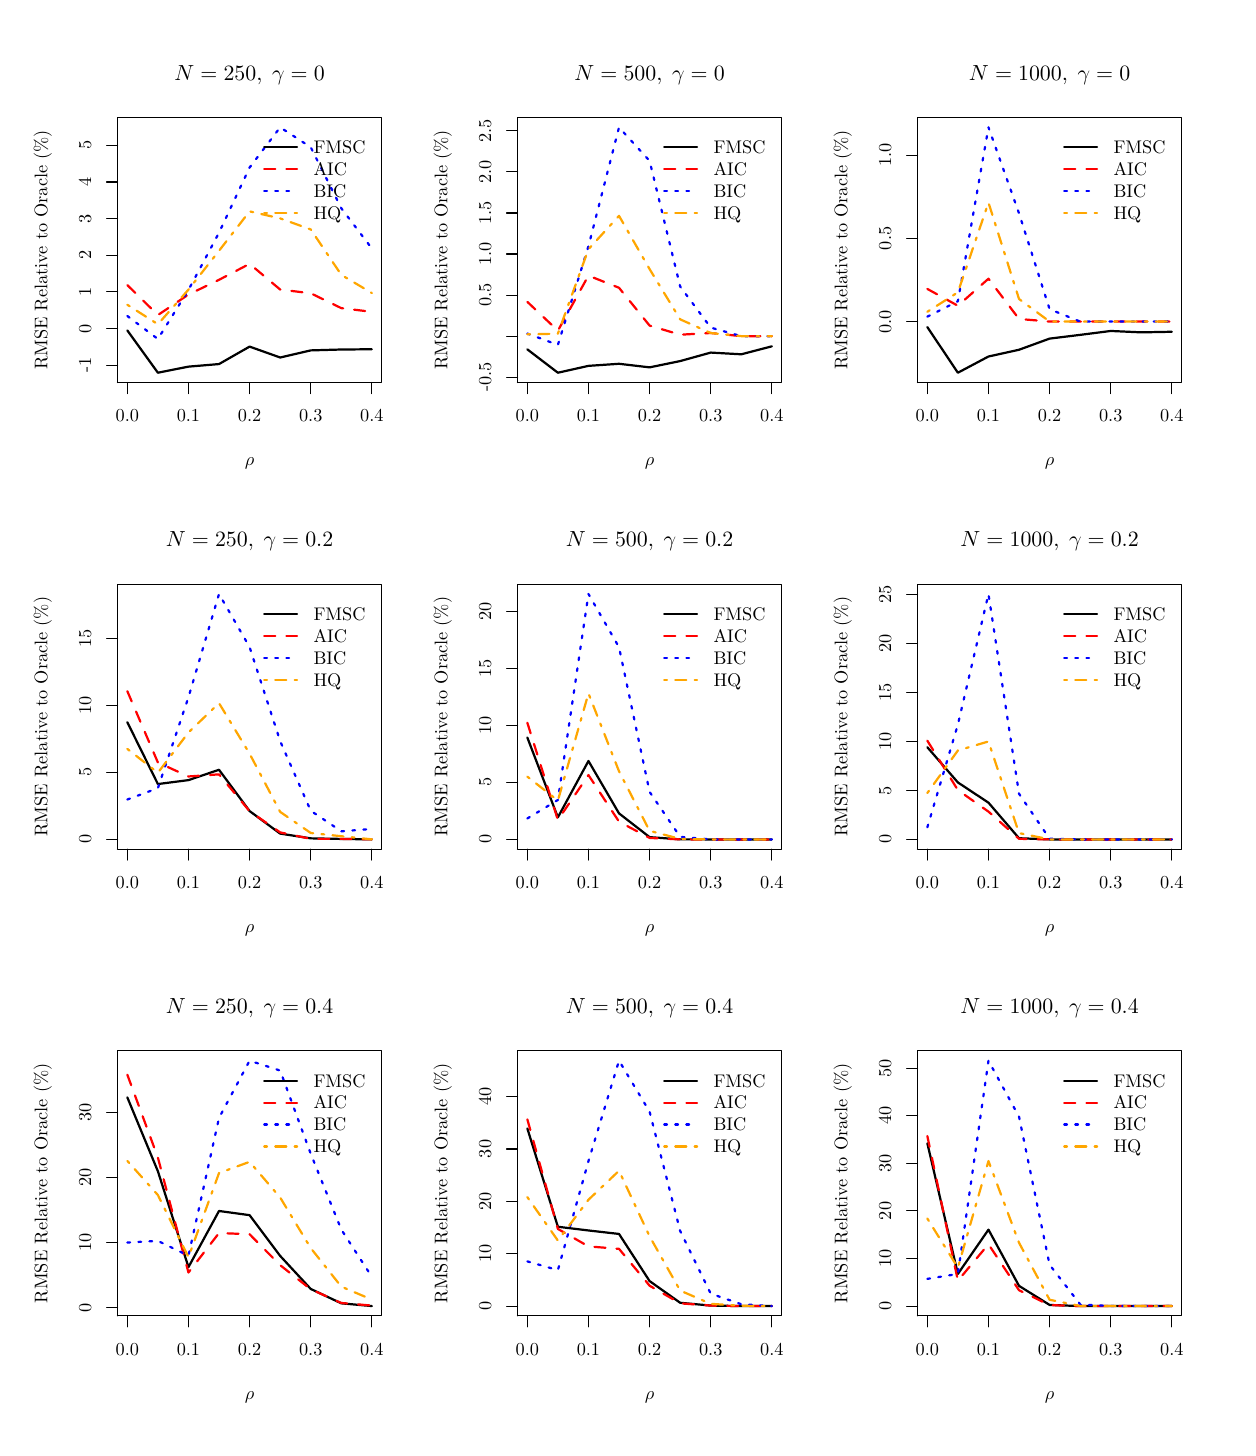
\begin{tikzpicture}[x=1pt,y=1pt]
\definecolor[named]{fillColor}{rgb}{1.00,1.00,1.00}
\path[use as bounding box,fill=fillColor,fill opacity=0.00] (0,0) rectangle (433.62,505.89);
\begin{scope}
\path[clip] ( 32.47,377.65) rectangle (127.91,473.42);
\definecolor[named]{drawColor}{rgb}{0.00,0.00,0.00}

\path[draw=drawColor,line width= 0.8pt,line join=round,line cap=round] ( 36.01,396.49) --
	( 47.05,381.20) --
	( 58.10,383.40) --
	( 69.14,384.33) --
	( 80.19,390.64) --
	( 91.24,386.70) --
	(102.28,389.27) --
	(113.33,389.59) --
	(124.37,389.68);
\end{scope}
\begin{scope}
\path[clip] (  0.00,  0.00) rectangle (433.62,505.89);
\definecolor[named]{drawColor}{rgb}{0.00,0.00,0.00}

\path[draw=drawColor,line width= 0.4pt,line join=round,line cap=round] ( 36.01,377.65) -- (124.37,377.65);

\path[draw=drawColor,line width= 0.4pt,line join=round,line cap=round] ( 36.01,377.65) -- ( 36.01,373.69);

\path[draw=drawColor,line width= 0.4pt,line join=round,line cap=round] ( 58.10,377.65) -- ( 58.10,373.69);

\path[draw=drawColor,line width= 0.4pt,line join=round,line cap=round] ( 80.19,377.65) -- ( 80.19,373.69);

\path[draw=drawColor,line width= 0.4pt,line join=round,line cap=round] (102.28,377.65) -- (102.28,373.69);

\path[draw=drawColor,line width= 0.4pt,line join=round,line cap=round] (124.37,377.65) -- (124.37,373.69);

\node[text=drawColor,anchor=base,inner sep=0pt, outer sep=0pt, scale=  0.66] at ( 36.01,363.40) {0.0};

\node[text=drawColor,anchor=base,inner sep=0pt, outer sep=0pt, scale=  0.66] at ( 58.10,363.40) {0.1};

\node[text=drawColor,anchor=base,inner sep=0pt, outer sep=0pt, scale=  0.66] at ( 80.19,363.40) {0.2};

\node[text=drawColor,anchor=base,inner sep=0pt, outer sep=0pt, scale=  0.66] at (102.28,363.40) {0.3};

\node[text=drawColor,anchor=base,inner sep=0pt, outer sep=0pt, scale=  0.66] at (124.37,363.40) {0.4};

\path[draw=drawColor,line width= 0.4pt,line join=round,line cap=round] ( 32.47,383.95) -- ( 32.47,463.36);

\path[draw=drawColor,line width= 0.4pt,line join=round,line cap=round] ( 32.47,383.95) -- ( 28.51,383.95);

\path[draw=drawColor,line width= 0.4pt,line join=round,line cap=round] ( 32.47,397.19) -- ( 28.51,397.19);

\path[draw=drawColor,line width= 0.4pt,line join=round,line cap=round] ( 32.47,410.42) -- ( 28.51,410.42);

\path[draw=drawColor,line width= 0.4pt,line join=round,line cap=round] ( 32.47,423.66) -- ( 28.51,423.66);

\path[draw=drawColor,line width= 0.4pt,line join=round,line cap=round] ( 32.47,436.89) -- ( 28.51,436.89);

\path[draw=drawColor,line width= 0.4pt,line join=round,line cap=round] ( 32.47,450.12) -- ( 28.51,450.12);

\path[draw=drawColor,line width= 0.4pt,line join=round,line cap=round] ( 32.47,463.36) -- ( 28.51,463.36);

\node[text=drawColor,rotate= 90.00,anchor=base,inner sep=0pt, outer sep=0pt, scale=  0.66] at ( 22.97,383.95) {-1};

\node[text=drawColor,rotate= 90.00,anchor=base,inner sep=0pt, outer sep=0pt, scale=  0.66] at ( 22.97,397.19) {0};

\node[text=drawColor,rotate= 90.00,anchor=base,inner sep=0pt, outer sep=0pt, scale=  0.66] at ( 22.97,410.42) {1};

\node[text=drawColor,rotate= 90.00,anchor=base,inner sep=0pt, outer sep=0pt, scale=  0.66] at ( 22.97,423.66) {2};

\node[text=drawColor,rotate= 90.00,anchor=base,inner sep=0pt, outer sep=0pt, scale=  0.66] at ( 22.97,436.89) {3};

\node[text=drawColor,rotate= 90.00,anchor=base,inner sep=0pt, outer sep=0pt, scale=  0.66] at ( 22.97,450.12) {4};

\node[text=drawColor,rotate= 90.00,anchor=base,inner sep=0pt, outer sep=0pt, scale=  0.66] at ( 22.97,463.36) {5};

\path[draw=drawColor,line width= 0.4pt,line join=round,line cap=round] ( 32.47,377.65) --
	(127.91,377.65) --
	(127.91,473.42) --
	( 32.47,473.42) --
	( 32.47,377.65);
\end{scope}
\begin{scope}
\path[clip] (  0.00,337.26) rectangle (144.54,505.89);
\definecolor[named]{drawColor}{rgb}{0.00,0.00,0.00}

\node[text=drawColor,anchor=base,inner sep=0pt, outer sep=0pt, scale=  0.79] at ( 80.19,486.92) {\bfseries $N=250, \;\gamma=0$};

\node[text=drawColor,anchor=base,inner sep=0pt, outer sep=0pt, scale=  0.66] at ( 80.19,347.56) {$\rho$};

\node[text=drawColor,rotate= 90.00,anchor=base,inner sep=0pt, outer sep=0pt, scale=  0.66] at (  7.13,425.53) {RMSE Relative to Oracle (\%)};
\end{scope}
\begin{scope}
\path[clip] ( 32.47,377.65) rectangle (127.91,473.42);
\definecolor[named]{drawColor}{rgb}{1.00,0.00,0.00}

\path[draw=drawColor,line width= 0.8pt,dash pattern=on 4pt off 4pt ,line join=round,line cap=round] ( 36.01,412.87) --
	( 47.05,402.05) --
	( 58.10,409.44) --
	( 69.14,414.77) --
	( 80.19,420.55) --
	( 91.24,411.26) --
	(102.28,409.91) --
	(113.33,404.54) --
	(124.37,403.21);
\definecolor[named]{drawColor}{rgb}{0.00,0.00,1.00}

\path[draw=drawColor,line width= 0.8pt,dash pattern=on 1pt off 3pt ,line join=round,line cap=round] ( 36.01,401.70) --
	( 47.05,393.38) --
	( 58.10,411.10) --
	( 69.14,431.79) --
	( 80.19,455.35) --
	( 91.24,469.87) --
	(102.28,462.69) --
	(113.33,440.62) --
	(124.37,426.10);
\definecolor[named]{drawColor}{rgb}{1.00,0.65,0.00}

\path[draw=drawColor,line width= 0.8pt,dash pattern=on 1pt off 3pt on 4pt off 3pt ,line join=round,line cap=round] ( 36.01,405.76) --
	( 47.05,398.72) --
	( 58.10,411.22) --
	( 69.14,425.26) --
	( 80.19,439.51) --
	( 91.24,436.97) --
	(102.28,432.98) --
	(113.33,416.56) --
	(124.37,409.99);
\definecolor[named]{drawColor}{rgb}{0.00,0.00,0.00}

\path[draw=drawColor,line width= 0.8pt,line join=round,line cap=round] ( 85.47,462.63) -- ( 97.35,462.63);
\definecolor[named]{drawColor}{rgb}{1.00,0.00,0.00}

\path[draw=drawColor,line width= 0.8pt,dash pattern=on 4pt off 4pt ,line join=round,line cap=round] ( 85.47,454.71) -- ( 97.35,454.71);
\definecolor[named]{drawColor}{rgb}{0.00,0.00,1.00}

\path[draw=drawColor,line width= 0.8pt,dash pattern=on 1pt off 3pt ,line join=round,line cap=round] ( 85.47,446.79) -- ( 97.35,446.79);
\definecolor[named]{drawColor}{rgb}{1.00,0.65,0.00}

\path[draw=drawColor,line width= 0.8pt,dash pattern=on 1pt off 3pt on 4pt off 3pt ,line join=round,line cap=round] ( 85.47,438.87) -- ( 97.35,438.87);
\definecolor[named]{drawColor}{rgb}{0.00,0.00,0.00}

\node[text=drawColor,anchor=base west,inner sep=0pt, outer sep=0pt, scale=  0.66] at (103.29,460.35) {FMSC};

\node[text=drawColor,anchor=base west,inner sep=0pt, outer sep=0pt, scale=  0.66] at (103.29,452.43) {AIC};

\node[text=drawColor,anchor=base west,inner sep=0pt, outer sep=0pt, scale=  0.66] at (103.29,444.51) {BIC};

\node[text=drawColor,anchor=base west,inner sep=0pt, outer sep=0pt, scale=  0.66] at (103.29,436.59) {HQ};
\end{scope}
\begin{scope}
\path[clip] (177.01,377.65) rectangle (272.45,473.42);
\definecolor[named]{drawColor}{rgb}{0.00,0.00,0.00}

\path[draw=drawColor,line width= 0.8pt,line join=round,line cap=round] (180.55,389.64) --
	(191.59,381.20) --
	(202.64,383.68) --
	(213.68,384.43) --
	(224.73,383.14) --
	(235.78,385.41) --
	(246.82,388.48) --
	(257.87,387.86) --
	(268.91,390.74);
\end{scope}
\begin{scope}
\path[clip] (  0.00,  0.00) rectangle (433.62,505.89);
\definecolor[named]{drawColor}{rgb}{0.00,0.00,0.00}

\path[draw=drawColor,line width= 0.4pt,line join=round,line cap=round] (180.55,377.65) -- (268.91,377.65);

\path[draw=drawColor,line width= 0.4pt,line join=round,line cap=round] (180.55,377.65) -- (180.55,373.69);

\path[draw=drawColor,line width= 0.4pt,line join=round,line cap=round] (202.64,377.65) -- (202.64,373.69);

\path[draw=drawColor,line width= 0.4pt,line join=round,line cap=round] (224.73,377.65) -- (224.73,373.69);

\path[draw=drawColor,line width= 0.4pt,line join=round,line cap=round] (246.82,377.65) -- (246.82,373.69);

\path[draw=drawColor,line width= 0.4pt,line join=round,line cap=round] (268.91,377.65) -- (268.91,373.69);

\node[text=drawColor,anchor=base,inner sep=0pt, outer sep=0pt, scale=  0.66] at (180.55,363.40) {0.0};

\node[text=drawColor,anchor=base,inner sep=0pt, outer sep=0pt, scale=  0.66] at (202.64,363.40) {0.1};

\node[text=drawColor,anchor=base,inner sep=0pt, outer sep=0pt, scale=  0.66] at (224.73,363.40) {0.2};

\node[text=drawColor,anchor=base,inner sep=0pt, outer sep=0pt, scale=  0.66] at (246.82,363.40) {0.3};

\node[text=drawColor,anchor=base,inner sep=0pt, outer sep=0pt, scale=  0.66] at (268.91,363.40) {0.4};

\path[draw=drawColor,line width= 0.4pt,line join=round,line cap=round] (177.01,379.57) -- (177.01,468.61);

\path[draw=drawColor,line width= 0.4pt,line join=round,line cap=round] (177.01,379.57) -- (173.05,379.57);

\path[draw=drawColor,line width= 0.4pt,line join=round,line cap=round] (177.01,394.41) -- (173.05,394.41);

\path[draw=drawColor,line width= 0.4pt,line join=round,line cap=round] (177.01,409.25) -- (173.05,409.25);

\path[draw=drawColor,line width= 0.4pt,line join=round,line cap=round] (177.01,424.09) -- (173.05,424.09);

\path[draw=drawColor,line width= 0.4pt,line join=round,line cap=round] (177.01,438.93) -- (173.05,438.93);

\path[draw=drawColor,line width= 0.4pt,line join=round,line cap=round] (177.01,453.77) -- (173.05,453.77);

\path[draw=drawColor,line width= 0.4pt,line join=round,line cap=round] (177.01,468.61) -- (173.05,468.61);

\node[text=drawColor,rotate= 90.00,anchor=base,inner sep=0pt, outer sep=0pt, scale=  0.66] at (167.51,379.57) {-0.5};

\node[text=drawColor,rotate= 90.00,anchor=base,inner sep=0pt, outer sep=0pt, scale=  0.66] at (167.51,409.25) {0.5};

\node[text=drawColor,rotate= 90.00,anchor=base,inner sep=0pt, outer sep=0pt, scale=  0.66] at (167.51,424.09) {1.0};

\node[text=drawColor,rotate= 90.00,anchor=base,inner sep=0pt, outer sep=0pt, scale=  0.66] at (167.51,438.93) {1.5};

\node[text=drawColor,rotate= 90.00,anchor=base,inner sep=0pt, outer sep=0pt, scale=  0.66] at (167.51,453.77) {2.0};

\node[text=drawColor,rotate= 90.00,anchor=base,inner sep=0pt, outer sep=0pt, scale=  0.66] at (167.51,468.61) {2.5};

\path[draw=drawColor,line width= 0.4pt,line join=round,line cap=round] (177.01,377.65) --
	(272.45,377.65) --
	(272.45,473.42) --
	(177.01,473.42) --
	(177.01,377.65);
\end{scope}
\begin{scope}
\path[clip] (144.54,337.26) rectangle (289.08,505.89);
\definecolor[named]{drawColor}{rgb}{0.00,0.00,0.00}

\node[text=drawColor,anchor=base,inner sep=0pt, outer sep=0pt, scale=  0.79] at (224.73,486.92) {\bfseries $N=500, \;\gamma=0$};

\node[text=drawColor,anchor=base,inner sep=0pt, outer sep=0pt, scale=  0.66] at (224.73,347.56) {$\rho$};

\node[text=drawColor,rotate= 90.00,anchor=base,inner sep=0pt, outer sep=0pt, scale=  0.66] at (151.67,425.53) {RMSE Relative to Oracle (\%)};
\end{scope}
\begin{scope}
\path[clip] (177.01,377.65) rectangle (272.45,473.42);
\definecolor[named]{drawColor}{rgb}{1.00,0.00,0.00}

\path[draw=drawColor,line width= 0.8pt,dash pattern=on 4pt off 4pt ,line join=round,line cap=round] (180.55,406.81) --
	(191.59,396.39) --
	(202.64,416.29) --
	(213.68,411.89) --
	(224.73,398.23) --
	(235.78,394.94) --
	(246.82,395.55) --
	(257.87,394.41) --
	(268.91,394.41);
\definecolor[named]{drawColor}{rgb}{0.00,0.00,1.00}

\path[draw=drawColor,line width= 0.8pt,dash pattern=on 1pt off 3pt ,line join=round,line cap=round] (180.55,395.37) --
	(191.59,391.25) --
	(202.64,426.93) --
	(213.68,469.87) --
	(224.73,457.75) --
	(235.78,412.35) --
	(246.82,397.50) --
	(257.87,394.41) --
	(268.91,394.41);
\definecolor[named]{drawColor}{rgb}{1.00,0.65,0.00}

\path[draw=drawColor,line width= 0.8pt,dash pattern=on 1pt off 3pt on 4pt off 3pt ,line join=round,line cap=round] (180.55,395.07) --
	(191.59,395.31) --
	(202.64,425.84) --
	(213.68,437.89) --
	(224.73,418.64) --
	(235.78,400.49) --
	(246.82,395.55) --
	(257.87,394.41) --
	(268.91,394.41);
\definecolor[named]{drawColor}{rgb}{0.00,0.00,0.00}

\path[draw=drawColor,line width= 0.8pt,line join=round,line cap=round] (230.01,462.63) -- (241.89,462.63);
\definecolor[named]{drawColor}{rgb}{1.00,0.00,0.00}

\path[draw=drawColor,line width= 0.8pt,dash pattern=on 4pt off 4pt ,line join=round,line cap=round] (230.01,454.71) -- (241.89,454.71);
\definecolor[named]{drawColor}{rgb}{0.00,0.00,1.00}

\path[draw=drawColor,line width= 0.8pt,dash pattern=on 1pt off 3pt ,line join=round,line cap=round] (230.01,446.79) -- (241.89,446.79);
\definecolor[named]{drawColor}{rgb}{1.00,0.65,0.00}

\path[draw=drawColor,line width= 0.8pt,dash pattern=on 1pt off 3pt on 4pt off 3pt ,line join=round,line cap=round] (230.01,438.87) -- (241.89,438.87);
\definecolor[named]{drawColor}{rgb}{0.00,0.00,0.00}

\node[text=drawColor,anchor=base west,inner sep=0pt, outer sep=0pt, scale=  0.66] at (247.83,460.35) {FMSC};

\node[text=drawColor,anchor=base west,inner sep=0pt, outer sep=0pt, scale=  0.66] at (247.83,452.43) {AIC};

\node[text=drawColor,anchor=base west,inner sep=0pt, outer sep=0pt, scale=  0.66] at (247.83,444.51) {BIC};

\node[text=drawColor,anchor=base west,inner sep=0pt, outer sep=0pt, scale=  0.66] at (247.83,436.59) {HQ};
\end{scope}
\begin{scope}
\path[clip] (321.55,377.65) rectangle (416.99,473.42);
\definecolor[named]{drawColor}{rgb}{0.00,0.00,0.00}

\path[draw=drawColor,line width= 0.8pt,line join=round,line cap=round] (325.09,397.69) --
	(336.13,381.20) --
	(347.18,387.06) --
	(358.22,389.50) --
	(369.27,393.53) --
	(380.32,394.88) --
	(391.36,396.29) --
	(402.41,395.79) --
	(413.45,396.00);
\end{scope}
\begin{scope}
\path[clip] (  0.00,  0.00) rectangle (433.62,505.89);
\definecolor[named]{drawColor}{rgb}{0.00,0.00,0.00}

\path[draw=drawColor,line width= 0.4pt,line join=round,line cap=round] (325.09,377.65) -- (413.45,377.65);

\path[draw=drawColor,line width= 0.4pt,line join=round,line cap=round] (325.09,377.65) -- (325.09,373.69);

\path[draw=drawColor,line width= 0.4pt,line join=round,line cap=round] (347.18,377.65) -- (347.18,373.69);

\path[draw=drawColor,line width= 0.4pt,line join=round,line cap=round] (369.27,377.65) -- (369.27,373.69);

\path[draw=drawColor,line width= 0.4pt,line join=round,line cap=round] (391.36,377.65) -- (391.36,373.69);

\path[draw=drawColor,line width= 0.4pt,line join=round,line cap=round] (413.45,377.65) -- (413.45,373.69);

\node[text=drawColor,anchor=base,inner sep=0pt, outer sep=0pt, scale=  0.66] at (325.09,363.40) {0.0};

\node[text=drawColor,anchor=base,inner sep=0pt, outer sep=0pt, scale=  0.66] at (347.18,363.40) {0.1};

\node[text=drawColor,anchor=base,inner sep=0pt, outer sep=0pt, scale=  0.66] at (369.27,363.40) {0.2};

\node[text=drawColor,anchor=base,inner sep=0pt, outer sep=0pt, scale=  0.66] at (391.36,363.40) {0.3};

\node[text=drawColor,anchor=base,inner sep=0pt, outer sep=0pt, scale=  0.66] at (413.45,363.40) {0.4};

\path[draw=drawColor,line width= 0.4pt,line join=round,line cap=round] (321.55,399.69) -- (321.55,459.81);

\path[draw=drawColor,line width= 0.4pt,line join=round,line cap=round] (321.55,399.69) -- (317.59,399.69);

\path[draw=drawColor,line width= 0.4pt,line join=round,line cap=round] (321.55,429.75) -- (317.59,429.75);

\path[draw=drawColor,line width= 0.4pt,line join=round,line cap=round] (321.55,459.81) -- (317.59,459.81);

\node[text=drawColor,rotate= 90.00,anchor=base,inner sep=0pt, outer sep=0pt, scale=  0.66] at (312.05,399.69) {0.0};

\node[text=drawColor,rotate= 90.00,anchor=base,inner sep=0pt, outer sep=0pt, scale=  0.66] at (312.05,429.75) {0.5};

\node[text=drawColor,rotate= 90.00,anchor=base,inner sep=0pt, outer sep=0pt, scale=  0.66] at (312.05,459.81) {1.0};

\path[draw=drawColor,line width= 0.4pt,line join=round,line cap=round] (321.55,377.65) --
	(416.99,377.65) --
	(416.99,473.42) --
	(321.55,473.42) --
	(321.55,377.65);
\end{scope}
\begin{scope}
\path[clip] (289.08,337.26) rectangle (433.62,505.89);
\definecolor[named]{drawColor}{rgb}{0.00,0.00,0.00}

\node[text=drawColor,anchor=base,inner sep=0pt, outer sep=0pt, scale=  0.79] at (369.27,486.92) {\bfseries $N=1000, \;\gamma=0$};

\node[text=drawColor,anchor=base,inner sep=0pt, outer sep=0pt, scale=  0.66] at (369.27,347.56) {$\rho$};

\node[text=drawColor,rotate= 90.00,anchor=base,inner sep=0pt, outer sep=0pt, scale=  0.66] at (296.21,425.53) {RMSE Relative to Oracle (\%)};
\end{scope}
\begin{scope}
\path[clip] (321.55,377.65) rectangle (416.99,473.42);
\definecolor[named]{drawColor}{rgb}{1.00,0.00,0.00}

\path[draw=drawColor,line width= 0.8pt,dash pattern=on 4pt off 4pt ,line join=round,line cap=round] (325.09,411.48) --
	(336.13,405.40) --
	(347.18,415.17) --
	(358.22,400.63) --
	(369.27,399.69) --
	(380.32,399.69) --
	(391.36,399.69) --
	(402.41,399.69) --
	(413.45,399.69);
\definecolor[named]{drawColor}{rgb}{0.00,0.00,1.00}

\path[draw=drawColor,line width= 0.8pt,dash pattern=on 1pt off 3pt ,line join=round,line cap=round] (325.09,401.45) --
	(336.13,407.03) --
	(347.18,469.87) --
	(358.22,438.81) --
	(369.27,404.16) --
	(380.32,399.69) --
	(391.36,399.69) --
	(402.41,399.69) --
	(413.45,399.69);
\definecolor[named]{drawColor}{rgb}{1.00,0.65,0.00}

\path[draw=drawColor,line width= 0.8pt,dash pattern=on 1pt off 3pt on 4pt off 3pt ,line join=round,line cap=round] (325.09,403.22) --
	(336.13,410.25) --
	(347.18,442.68) --
	(358.22,407.84) --
	(369.27,399.69) --
	(380.32,399.69) --
	(391.36,399.69) --
	(402.41,399.69) --
	(413.45,399.69);
\definecolor[named]{drawColor}{rgb}{0.00,0.00,0.00}

\path[draw=drawColor,line width= 0.8pt,line join=round,line cap=round] (374.55,462.63) -- (386.43,462.63);
\definecolor[named]{drawColor}{rgb}{1.00,0.00,0.00}

\path[draw=drawColor,line width= 0.8pt,dash pattern=on 4pt off 4pt ,line join=round,line cap=round] (374.55,454.71) -- (386.43,454.71);
\definecolor[named]{drawColor}{rgb}{0.00,0.00,1.00}

\path[draw=drawColor,line width= 0.8pt,dash pattern=on 1pt off 3pt ,line join=round,line cap=round] (374.55,446.79) -- (386.43,446.79);
\definecolor[named]{drawColor}{rgb}{1.00,0.65,0.00}

\path[draw=drawColor,line width= 0.8pt,dash pattern=on 1pt off 3pt on 4pt off 3pt ,line join=round,line cap=round] (374.55,438.87) -- (386.43,438.87);
\definecolor[named]{drawColor}{rgb}{0.00,0.00,0.00}

\node[text=drawColor,anchor=base west,inner sep=0pt, outer sep=0pt, scale=  0.66] at (392.37,460.35) {FMSC};

\node[text=drawColor,anchor=base west,inner sep=0pt, outer sep=0pt, scale=  0.66] at (392.37,452.43) {AIC};

\node[text=drawColor,anchor=base west,inner sep=0pt, outer sep=0pt, scale=  0.66] at (392.37,444.51) {BIC};

\node[text=drawColor,anchor=base west,inner sep=0pt, outer sep=0pt, scale=  0.66] at (392.37,436.59) {HQ};
\end{scope}
\begin{scope}
\path[clip] ( 32.47,209.02) rectangle (127.91,304.79);
\definecolor[named]{drawColor}{rgb}{0.00,0.00,0.00}

\path[draw=drawColor,line width= 0.8pt,line join=round,line cap=round] ( 36.01,254.91) --
	( 47.05,232.57) --
	( 58.10,233.99) --
	( 69.14,237.73) --
	( 80.19,222.81) --
	( 91.24,214.66) --
	(102.28,212.95) --
	(113.33,212.74) --
	(124.37,212.57);
\end{scope}
\begin{scope}
\path[clip] (  0.00,  0.00) rectangle (433.62,505.89);
\definecolor[named]{drawColor}{rgb}{0.00,0.00,0.00}

\path[draw=drawColor,line width= 0.4pt,line join=round,line cap=round] ( 36.01,209.02) -- (124.37,209.02);

\path[draw=drawColor,line width= 0.4pt,line join=round,line cap=round] ( 36.01,209.02) -- ( 36.01,205.06);

\path[draw=drawColor,line width= 0.4pt,line join=round,line cap=round] ( 58.10,209.02) -- ( 58.10,205.06);

\path[draw=drawColor,line width= 0.4pt,line join=round,line cap=round] ( 80.19,209.02) -- ( 80.19,205.06);

\path[draw=drawColor,line width= 0.4pt,line join=round,line cap=round] (102.28,209.02) -- (102.28,205.06);

\path[draw=drawColor,line width= 0.4pt,line join=round,line cap=round] (124.37,209.02) -- (124.37,205.06);

\node[text=drawColor,anchor=base,inner sep=0pt, outer sep=0pt, scale=  0.66] at ( 36.01,194.77) {0.0};

\node[text=drawColor,anchor=base,inner sep=0pt, outer sep=0pt, scale=  0.66] at ( 58.10,194.77) {0.1};

\node[text=drawColor,anchor=base,inner sep=0pt, outer sep=0pt, scale=  0.66] at ( 80.19,194.77) {0.2};

\node[text=drawColor,anchor=base,inner sep=0pt, outer sep=0pt, scale=  0.66] at (102.28,194.77) {0.3};

\node[text=drawColor,anchor=base,inner sep=0pt, outer sep=0pt, scale=  0.66] at (124.37,194.77) {0.4};

\path[draw=drawColor,line width= 0.4pt,line join=round,line cap=round] ( 32.47,212.59) -- ( 32.47,285.16);

\path[draw=drawColor,line width= 0.4pt,line join=round,line cap=round] ( 32.47,212.59) -- ( 28.51,212.59);

\path[draw=drawColor,line width= 0.4pt,line join=round,line cap=round] ( 32.47,236.78) -- ( 28.51,236.78);

\path[draw=drawColor,line width= 0.4pt,line join=round,line cap=round] ( 32.47,260.97) -- ( 28.51,260.97);

\path[draw=drawColor,line width= 0.4pt,line join=round,line cap=round] ( 32.47,285.16) -- ( 28.51,285.16);

\node[text=drawColor,rotate= 90.00,anchor=base,inner sep=0pt, outer sep=0pt, scale=  0.66] at ( 22.97,212.59) {0};

\node[text=drawColor,rotate= 90.00,anchor=base,inner sep=0pt, outer sep=0pt, scale=  0.66] at ( 22.97,236.78) {5};

\node[text=drawColor,rotate= 90.00,anchor=base,inner sep=0pt, outer sep=0pt, scale=  0.66] at ( 22.97,260.97) {10};

\node[text=drawColor,rotate= 90.00,anchor=base,inner sep=0pt, outer sep=0pt, scale=  0.66] at ( 22.97,285.16) {15};

\path[draw=drawColor,line width= 0.4pt,line join=round,line cap=round] ( 32.47,209.02) --
	(127.91,209.02) --
	(127.91,304.79) --
	( 32.47,304.79) --
	( 32.47,209.02);
\end{scope}
\begin{scope}
\path[clip] (  0.00,168.63) rectangle (144.54,337.26);
\definecolor[named]{drawColor}{rgb}{0.00,0.00,0.00}

\node[text=drawColor,anchor=base,inner sep=0pt, outer sep=0pt, scale=  0.79] at ( 80.19,318.29) {\bfseries $N=250, \;\gamma=0.2$};

\node[text=drawColor,anchor=base,inner sep=0pt, outer sep=0pt, scale=  0.66] at ( 80.19,178.93) {$\rho$};

\node[text=drawColor,rotate= 90.00,anchor=base,inner sep=0pt, outer sep=0pt, scale=  0.66] at (  7.13,256.90) {RMSE Relative to Oracle (\%)};
\end{scope}
\begin{scope}
\path[clip] ( 32.47,209.02) rectangle (127.91,304.79);
\definecolor[named]{drawColor}{rgb}{1.00,0.00,0.00}

\path[draw=drawColor,line width= 0.8pt,dash pattern=on 4pt off 4pt ,line join=round,line cap=round] ( 36.01,266.12) --
	( 47.05,240.36) --
	( 58.10,235.31) --
	( 69.14,236.07) --
	( 80.19,222.76) --
	( 91.24,215.10) --
	(102.28,212.76) --
	(113.33,212.76) --
	(124.37,212.59);
\definecolor[named]{drawColor}{rgb}{0.00,0.00,1.00}

\path[draw=drawColor,line width= 0.8pt,dash pattern=on 1pt off 3pt ,line join=round,line cap=round] ( 36.01,226.98) --
	( 47.05,231.09) --
	( 58.10,263.94) --
	( 69.14,301.24) --
	( 80.19,282.08) --
	( 91.24,248.07) --
	(102.28,222.93) --
	(113.33,215.49) --
	(124.37,216.35);
\definecolor[named]{drawColor}{rgb}{1.00,0.65,0.00}

\path[draw=drawColor,line width= 0.8pt,dash pattern=on 1pt off 3pt on 4pt off 3pt ,line join=round,line cap=round] ( 36.01,245.26) --
	( 47.05,236.64) --
	( 58.10,251.20) --
	( 69.14,261.81) --
	( 80.19,243.54) --
	( 91.24,222.52) --
	(102.28,214.89) --
	(113.33,213.72) --
	(124.37,212.59);
\definecolor[named]{drawColor}{rgb}{0.00,0.00,0.00}

\path[draw=drawColor,line width= 0.8pt,line join=round,line cap=round] ( 85.47,294.00) -- ( 97.35,294.00);
\definecolor[named]{drawColor}{rgb}{1.00,0.00,0.00}

\path[draw=drawColor,line width= 0.8pt,dash pattern=on 4pt off 4pt ,line join=round,line cap=round] ( 85.47,286.08) -- ( 97.35,286.08);
\definecolor[named]{drawColor}{rgb}{0.00,0.00,1.00}

\path[draw=drawColor,line width= 0.8pt,dash pattern=on 1pt off 3pt ,line join=round,line cap=round] ( 85.47,278.16) -- ( 97.35,278.16);
\definecolor[named]{drawColor}{rgb}{1.00,0.65,0.00}

\path[draw=drawColor,line width= 0.8pt,dash pattern=on 1pt off 3pt on 4pt off 3pt ,line join=round,line cap=round] ( 85.47,270.24) -- ( 97.35,270.24);
\definecolor[named]{drawColor}{rgb}{0.00,0.00,0.00}

\node[text=drawColor,anchor=base west,inner sep=0pt, outer sep=0pt, scale=  0.66] at (103.29,291.72) {FMSC};

\node[text=drawColor,anchor=base west,inner sep=0pt, outer sep=0pt, scale=  0.66] at (103.29,283.80) {AIC};

\node[text=drawColor,anchor=base west,inner sep=0pt, outer sep=0pt, scale=  0.66] at (103.29,275.88) {BIC};

\node[text=drawColor,anchor=base west,inner sep=0pt, outer sep=0pt, scale=  0.66] at (103.29,267.96) {HQ};
\end{scope}
\begin{scope}
\path[clip] (177.01,209.02) rectangle (272.45,304.79);
\definecolor[named]{drawColor}{rgb}{0.00,0.00,0.00}

\path[draw=drawColor,line width= 0.8pt,line join=round,line cap=round] (180.55,249.38) --
	(191.59,220.54) --
	(202.64,240.91) --
	(213.68,221.97) --
	(224.73,213.39) --
	(235.78,212.58) --
	(246.82,212.57) --
	(257.87,212.57) --
	(268.91,212.57);
\end{scope}
\begin{scope}
\path[clip] (  0.00,  0.00) rectangle (433.62,505.89);
\definecolor[named]{drawColor}{rgb}{0.00,0.00,0.00}

\path[draw=drawColor,line width= 0.4pt,line join=round,line cap=round] (180.55,209.02) -- (268.91,209.02);

\path[draw=drawColor,line width= 0.4pt,line join=round,line cap=round] (180.55,209.02) -- (180.55,205.06);

\path[draw=drawColor,line width= 0.4pt,line join=round,line cap=round] (202.64,209.02) -- (202.64,205.06);

\path[draw=drawColor,line width= 0.4pt,line join=round,line cap=round] (224.73,209.02) -- (224.73,205.06);

\path[draw=drawColor,line width= 0.4pt,line join=round,line cap=round] (246.82,209.02) -- (246.82,205.06);

\path[draw=drawColor,line width= 0.4pt,line join=round,line cap=round] (268.91,209.02) -- (268.91,205.06);

\node[text=drawColor,anchor=base,inner sep=0pt, outer sep=0pt, scale=  0.66] at (180.55,194.77) {0.0};

\node[text=drawColor,anchor=base,inner sep=0pt, outer sep=0pt, scale=  0.66] at (202.64,194.77) {0.1};

\node[text=drawColor,anchor=base,inner sep=0pt, outer sep=0pt, scale=  0.66] at (224.73,194.77) {0.2};

\node[text=drawColor,anchor=base,inner sep=0pt, outer sep=0pt, scale=  0.66] at (246.82,194.77) {0.3};

\node[text=drawColor,anchor=base,inner sep=0pt, outer sep=0pt, scale=  0.66] at (268.91,194.77) {0.4};

\path[draw=drawColor,line width= 0.4pt,line join=round,line cap=round] (177.01,212.57) -- (177.01,295.01);

\path[draw=drawColor,line width= 0.4pt,line join=round,line cap=round] (177.01,212.57) -- (173.05,212.57);

\path[draw=drawColor,line width= 0.4pt,line join=round,line cap=round] (177.01,233.18) -- (173.05,233.18);

\path[draw=drawColor,line width= 0.4pt,line join=round,line cap=round] (177.01,253.79) -- (173.05,253.79);

\path[draw=drawColor,line width= 0.4pt,line join=round,line cap=round] (177.01,274.40) -- (173.05,274.40);

\path[draw=drawColor,line width= 0.4pt,line join=round,line cap=round] (177.01,295.01) -- (173.05,295.01);

\node[text=drawColor,rotate= 90.00,anchor=base,inner sep=0pt, outer sep=0pt, scale=  0.66] at (167.51,212.57) {0};

\node[text=drawColor,rotate= 90.00,anchor=base,inner sep=0pt, outer sep=0pt, scale=  0.66] at (167.51,233.18) {5};

\node[text=drawColor,rotate= 90.00,anchor=base,inner sep=0pt, outer sep=0pt, scale=  0.66] at (167.51,253.79) {10};

\node[text=drawColor,rotate= 90.00,anchor=base,inner sep=0pt, outer sep=0pt, scale=  0.66] at (167.51,274.40) {15};

\node[text=drawColor,rotate= 90.00,anchor=base,inner sep=0pt, outer sep=0pt, scale=  0.66] at (167.51,295.01) {20};

\path[draw=drawColor,line width= 0.4pt,line join=round,line cap=round] (177.01,209.02) --
	(272.45,209.02) --
	(272.45,304.79) --
	(177.01,304.79) --
	(177.01,209.02);
\end{scope}
\begin{scope}
\path[clip] (144.54,168.63) rectangle (289.08,337.26);
\definecolor[named]{drawColor}{rgb}{0.00,0.00,0.00}

\node[text=drawColor,anchor=base,inner sep=0pt, outer sep=0pt, scale=  0.79] at (224.73,318.29) {\bfseries $N=500, \;\gamma=0.2$};

\node[text=drawColor,anchor=base,inner sep=0pt, outer sep=0pt, scale=  0.66] at (224.73,178.93) {$\rho$};

\node[text=drawColor,rotate= 90.00,anchor=base,inner sep=0pt, outer sep=0pt, scale=  0.66] at (151.67,256.90) {RMSE Relative to Oracle (\%)};
\end{scope}
\begin{scope}
\path[clip] (177.01,209.02) rectangle (272.45,304.79);
\definecolor[named]{drawColor}{rgb}{1.00,0.00,0.00}

\path[draw=drawColor,line width= 0.8pt,dash pattern=on 4pt off 4pt ,line join=round,line cap=round] (180.55,254.72) --
	(191.59,219.59) --
	(202.64,235.82) --
	(213.68,218.97) --
	(224.73,213.10) --
	(235.78,212.57) --
	(246.82,212.57) --
	(257.87,212.57) --
	(268.91,212.57);
\definecolor[named]{drawColor}{rgb}{0.00,0.00,1.00}

\path[draw=drawColor,line width= 0.8pt,dash pattern=on 1pt off 3pt ,line join=round,line cap=round] (180.55,220.13) --
	(191.59,226.82) --
	(202.64,301.24) --
	(213.68,282.01) --
	(224.73,229.74) --
	(235.78,213.49) --
	(246.82,212.57) --
	(257.87,212.57) --
	(268.91,212.57);
\definecolor[named]{drawColor}{rgb}{1.00,0.65,0.00}

\path[draw=drawColor,line width= 0.8pt,dash pattern=on 1pt off 3pt on 4pt off 3pt ,line join=round,line cap=round] (180.55,235.25) --
	(191.59,226.61) --
	(202.64,265.34) --
	(213.68,237.18) --
	(224.73,215.66) --
	(235.78,212.74) --
	(246.82,212.57) --
	(257.87,212.57) --
	(268.91,212.57);
\definecolor[named]{drawColor}{rgb}{0.00,0.00,0.00}

\path[draw=drawColor,line width= 0.8pt,line join=round,line cap=round] (230.01,294.00) -- (241.89,294.00);
\definecolor[named]{drawColor}{rgb}{1.00,0.00,0.00}

\path[draw=drawColor,line width= 0.8pt,dash pattern=on 4pt off 4pt ,line join=round,line cap=round] (230.01,286.08) -- (241.89,286.08);
\definecolor[named]{drawColor}{rgb}{0.00,0.00,1.00}

\path[draw=drawColor,line width= 0.8pt,dash pattern=on 1pt off 3pt ,line join=round,line cap=round] (230.01,278.16) -- (241.89,278.16);
\definecolor[named]{drawColor}{rgb}{1.00,0.65,0.00}

\path[draw=drawColor,line width= 0.8pt,dash pattern=on 1pt off 3pt on 4pt off 3pt ,line join=round,line cap=round] (230.01,270.24) -- (241.89,270.24);
\definecolor[named]{drawColor}{rgb}{0.00,0.00,0.00}

\node[text=drawColor,anchor=base west,inner sep=0pt, outer sep=0pt, scale=  0.66] at (247.83,291.72) {FMSC};

\node[text=drawColor,anchor=base west,inner sep=0pt, outer sep=0pt, scale=  0.66] at (247.83,283.80) {AIC};

\node[text=drawColor,anchor=base west,inner sep=0pt, outer sep=0pt, scale=  0.66] at (247.83,275.88) {BIC};

\node[text=drawColor,anchor=base west,inner sep=0pt, outer sep=0pt, scale=  0.66] at (247.83,267.96) {HQ};
\end{scope}
\begin{scope}
\path[clip] (321.55,209.02) rectangle (416.99,304.79);
\definecolor[named]{drawColor}{rgb}{0.00,0.00,0.00}

\path[draw=drawColor,line width= 0.8pt,line join=round,line cap=round] (325.09,245.87) --
	(336.13,233.15) --
	(347.18,225.84) --
	(358.22,212.99) --
	(369.27,212.57) --
	(380.32,212.57) --
	(391.36,212.57) --
	(402.41,212.57) --
	(413.45,212.57);
\end{scope}
\begin{scope}
\path[clip] (  0.00,  0.00) rectangle (433.62,505.89);
\definecolor[named]{drawColor}{rgb}{0.00,0.00,0.00}

\path[draw=drawColor,line width= 0.4pt,line join=round,line cap=round] (325.09,209.02) -- (413.45,209.02);

\path[draw=drawColor,line width= 0.4pt,line join=round,line cap=round] (325.09,209.02) -- (325.09,205.06);

\path[draw=drawColor,line width= 0.4pt,line join=round,line cap=round] (347.18,209.02) -- (347.18,205.06);

\path[draw=drawColor,line width= 0.4pt,line join=round,line cap=round] (369.27,209.02) -- (369.27,205.06);

\path[draw=drawColor,line width= 0.4pt,line join=round,line cap=round] (391.36,209.02) -- (391.36,205.06);

\path[draw=drawColor,line width= 0.4pt,line join=round,line cap=round] (413.45,209.02) -- (413.45,205.06);

\node[text=drawColor,anchor=base,inner sep=0pt, outer sep=0pt, scale=  0.66] at (325.09,194.77) {0.0};

\node[text=drawColor,anchor=base,inner sep=0pt, outer sep=0pt, scale=  0.66] at (347.18,194.77) {0.1};

\node[text=drawColor,anchor=base,inner sep=0pt, outer sep=0pt, scale=  0.66] at (369.27,194.77) {0.2};

\node[text=drawColor,anchor=base,inner sep=0pt, outer sep=0pt, scale=  0.66] at (391.36,194.77) {0.3};

\node[text=drawColor,anchor=base,inner sep=0pt, outer sep=0pt, scale=  0.66] at (413.45,194.77) {0.4};

\path[draw=drawColor,line width= 0.4pt,line join=round,line cap=round] (321.55,212.57) -- (321.55,301.05);

\path[draw=drawColor,line width= 0.4pt,line join=round,line cap=round] (321.55,212.57) -- (317.59,212.57);

\path[draw=drawColor,line width= 0.4pt,line join=round,line cap=round] (321.55,230.26) -- (317.59,230.26);

\path[draw=drawColor,line width= 0.4pt,line join=round,line cap=round] (321.55,247.96) -- (317.59,247.96);

\path[draw=drawColor,line width= 0.4pt,line join=round,line cap=round] (321.55,265.66) -- (317.59,265.66);

\path[draw=drawColor,line width= 0.4pt,line join=round,line cap=round] (321.55,283.35) -- (317.59,283.35);

\path[draw=drawColor,line width= 0.4pt,line join=round,line cap=round] (321.55,301.05) -- (317.59,301.05);

\node[text=drawColor,rotate= 90.00,anchor=base,inner sep=0pt, outer sep=0pt, scale=  0.66] at (312.05,212.57) {0};

\node[text=drawColor,rotate= 90.00,anchor=base,inner sep=0pt, outer sep=0pt, scale=  0.66] at (312.05,230.26) {5};

\node[text=drawColor,rotate= 90.00,anchor=base,inner sep=0pt, outer sep=0pt, scale=  0.66] at (312.05,247.96) {10};

\node[text=drawColor,rotate= 90.00,anchor=base,inner sep=0pt, outer sep=0pt, scale=  0.66] at (312.05,265.66) {15};

\node[text=drawColor,rotate= 90.00,anchor=base,inner sep=0pt, outer sep=0pt, scale=  0.66] at (312.05,283.35) {20};

\node[text=drawColor,rotate= 90.00,anchor=base,inner sep=0pt, outer sep=0pt, scale=  0.66] at (312.05,301.05) {25};

\path[draw=drawColor,line width= 0.4pt,line join=round,line cap=round] (321.55,209.02) --
	(416.99,209.02) --
	(416.99,304.79) --
	(321.55,304.79) --
	(321.55,209.02);
\end{scope}
\begin{scope}
\path[clip] (289.08,168.63) rectangle (433.62,337.26);
\definecolor[named]{drawColor}{rgb}{0.00,0.00,0.00}

\node[text=drawColor,anchor=base,inner sep=0pt, outer sep=0pt, scale=  0.79] at (369.27,318.29) {\bfseries $N=1000, \;\gamma=0.2$};

\node[text=drawColor,anchor=base,inner sep=0pt, outer sep=0pt, scale=  0.66] at (369.27,178.93) {$\rho$};

\node[text=drawColor,rotate= 90.00,anchor=base,inner sep=0pt, outer sep=0pt, scale=  0.66] at (296.21,256.90) {RMSE Relative to Oracle (\%)};
\end{scope}
\begin{scope}
\path[clip] (321.55,209.02) rectangle (416.99,304.79);
\definecolor[named]{drawColor}{rgb}{1.00,0.00,0.00}

\path[draw=drawColor,line width= 0.8pt,dash pattern=on 4pt off 4pt ,line join=round,line cap=round] (325.09,248.24) --
	(336.13,230.38) --
	(347.18,222.61) --
	(358.22,212.78) --
	(369.27,212.57) --
	(380.32,212.57) --
	(391.36,212.57) --
	(402.41,212.57) --
	(413.45,212.57);
\definecolor[named]{drawColor}{rgb}{0.00,0.00,1.00}

\path[draw=drawColor,line width= 0.8pt,dash pattern=on 1pt off 3pt ,line join=round,line cap=round] (325.09,216.95) --
	(336.13,254.09) --
	(347.18,301.24) --
	(358.22,229.07) --
	(369.27,212.80) --
	(380.32,212.57) --
	(391.36,212.57) --
	(402.41,212.57) --
	(413.45,212.57);
\definecolor[named]{drawColor}{rgb}{1.00,0.65,0.00}

\path[draw=drawColor,line width= 0.8pt,dash pattern=on 1pt off 3pt on 4pt off 3pt ,line join=round,line cap=round] (325.09,229.32) --
	(336.13,244.70) --
	(347.18,247.96) --
	(358.22,214.85) --
	(369.27,212.57) --
	(380.32,212.57) --
	(391.36,212.57) --
	(402.41,212.57) --
	(413.45,212.57);
\definecolor[named]{drawColor}{rgb}{0.00,0.00,0.00}

\path[draw=drawColor,line width= 0.8pt,line join=round,line cap=round] (374.55,294.00) -- (386.43,294.00);
\definecolor[named]{drawColor}{rgb}{1.00,0.00,0.00}

\path[draw=drawColor,line width= 0.8pt,dash pattern=on 4pt off 4pt ,line join=round,line cap=round] (374.55,286.08) -- (386.43,286.08);
\definecolor[named]{drawColor}{rgb}{0.00,0.00,1.00}

\path[draw=drawColor,line width= 0.8pt,dash pattern=on 1pt off 3pt ,line join=round,line cap=round] (374.55,278.16) -- (386.43,278.16);
\definecolor[named]{drawColor}{rgb}{1.00,0.65,0.00}

\path[draw=drawColor,line width= 0.8pt,dash pattern=on 1pt off 3pt on 4pt off 3pt ,line join=round,line cap=round] (374.55,270.24) -- (386.43,270.24);
\definecolor[named]{drawColor}{rgb}{0.00,0.00,0.00}

\node[text=drawColor,anchor=base west,inner sep=0pt, outer sep=0pt, scale=  0.66] at (392.37,291.72) {FMSC};

\node[text=drawColor,anchor=base west,inner sep=0pt, outer sep=0pt, scale=  0.66] at (392.37,283.80) {AIC};

\node[text=drawColor,anchor=base west,inner sep=0pt, outer sep=0pt, scale=  0.66] at (392.37,275.88) {BIC};

\node[text=drawColor,anchor=base west,inner sep=0pt, outer sep=0pt, scale=  0.66] at (392.37,267.96) {HQ};
\end{scope}
\begin{scope}
\path[clip] ( 32.47, 40.39) rectangle (127.91,136.16);
\definecolor[named]{drawColor}{rgb}{0.00,0.00,0.00}

\path[draw=drawColor,line width= 0.8pt,line join=round,line cap=round] ( 36.01,119.35) --
	( 47.05, 92.66) --
	( 58.10, 58.02) --
	( 69.14, 78.30) --
	( 80.19, 76.79) --
	( 91.24, 62.06) --
	(102.28, 50.13) --
	(113.33, 44.93) --
	(124.37, 43.94);
\end{scope}
\begin{scope}
\path[clip] (  0.00,  0.00) rectangle (433.62,505.89);
\definecolor[named]{drawColor}{rgb}{0.00,0.00,0.00}

\path[draw=drawColor,line width= 0.4pt,line join=round,line cap=round] ( 36.01, 40.39) -- (124.37, 40.39);

\path[draw=drawColor,line width= 0.4pt,line join=round,line cap=round] ( 36.01, 40.39) -- ( 36.01, 36.43);

\path[draw=drawColor,line width= 0.4pt,line join=round,line cap=round] ( 58.10, 40.39) -- ( 58.10, 36.43);

\path[draw=drawColor,line width= 0.4pt,line join=round,line cap=round] ( 80.19, 40.39) -- ( 80.19, 36.43);

\path[draw=drawColor,line width= 0.4pt,line join=round,line cap=round] (102.28, 40.39) -- (102.28, 36.43);

\path[draw=drawColor,line width= 0.4pt,line join=round,line cap=round] (124.37, 40.39) -- (124.37, 36.43);

\node[text=drawColor,anchor=base,inner sep=0pt, outer sep=0pt, scale=  0.66] at ( 36.01, 26.14) {0.0};

\node[text=drawColor,anchor=base,inner sep=0pt, outer sep=0pt, scale=  0.66] at ( 58.10, 26.14) {0.1};

\node[text=drawColor,anchor=base,inner sep=0pt, outer sep=0pt, scale=  0.66] at ( 80.19, 26.14) {0.2};

\node[text=drawColor,anchor=base,inner sep=0pt, outer sep=0pt, scale=  0.66] at (102.28, 26.14) {0.3};

\node[text=drawColor,anchor=base,inner sep=0pt, outer sep=0pt, scale=  0.66] at (124.37, 26.14) {0.4};

\path[draw=drawColor,line width= 0.4pt,line join=round,line cap=round] ( 32.47, 43.44) -- ( 32.47,113.94);

\path[draw=drawColor,line width= 0.4pt,line join=round,line cap=round] ( 32.47, 43.44) -- ( 28.51, 43.44);

\path[draw=drawColor,line width= 0.4pt,line join=round,line cap=round] ( 32.47, 66.94) -- ( 28.51, 66.94);

\path[draw=drawColor,line width= 0.4pt,line join=round,line cap=round] ( 32.47, 90.44) -- ( 28.51, 90.44);

\path[draw=drawColor,line width= 0.4pt,line join=round,line cap=round] ( 32.47,113.94) -- ( 28.51,113.94);

\node[text=drawColor,rotate= 90.00,anchor=base,inner sep=0pt, outer sep=0pt, scale=  0.66] at ( 22.97, 43.44) {0};

\node[text=drawColor,rotate= 90.00,anchor=base,inner sep=0pt, outer sep=0pt, scale=  0.66] at ( 22.97, 66.94) {10};

\node[text=drawColor,rotate= 90.00,anchor=base,inner sep=0pt, outer sep=0pt, scale=  0.66] at ( 22.97, 90.44) {20};

\node[text=drawColor,rotate= 90.00,anchor=base,inner sep=0pt, outer sep=0pt, scale=  0.66] at ( 22.97,113.94) {30};

\path[draw=drawColor,line width= 0.4pt,line join=round,line cap=round] ( 32.47, 40.39) --
	(127.91, 40.39) --
	(127.91,136.16) --
	( 32.47,136.16) --
	( 32.47, 40.39);
\end{scope}
\begin{scope}
\path[clip] (  0.00,  0.00) rectangle (144.54,168.63);
\definecolor[named]{drawColor}{rgb}{0.00,0.00,0.00}

\node[text=drawColor,anchor=base,inner sep=0pt, outer sep=0pt, scale=  0.79] at ( 80.19,149.66) {\bfseries $N=250, \;\gamma=0.4$};

\node[text=drawColor,anchor=base,inner sep=0pt, outer sep=0pt, scale=  0.66] at ( 80.19, 10.30) {$\rho$};

\node[text=drawColor,rotate= 90.00,anchor=base,inner sep=0pt, outer sep=0pt, scale=  0.66] at (  7.13, 88.27) {RMSE Relative to Oracle (\%)};
\end{scope}
\begin{scope}
\path[clip] ( 32.47, 40.39) rectangle (127.91,136.16);
\definecolor[named]{drawColor}{rgb}{1.00,0.00,0.00}

\path[draw=drawColor,line width= 0.8pt,dash pattern=on 4pt off 4pt ,line join=round,line cap=round] ( 36.01,127.54) --
	( 47.05, 97.60) --
	( 58.10, 56.06) --
	( 69.14, 70.34) --
	( 80.19, 69.89) --
	( 91.24, 58.72) --
	(102.28, 50.01) --
	(113.33, 45.06) --
	(124.37, 44.12);
\definecolor[named]{drawColor}{rgb}{0.00,0.00,1.00}

\path[draw=drawColor,line width= 0.8pt,dash pattern=on 1pt off 3pt ,line join=round,line cap=round] ( 36.01, 66.90) --
	( 47.05, 67.50) --
	( 58.10, 62.13) --
	( 69.14,111.93) --
	( 80.19,132.61) --
	( 91.24,129.04) --
	(102.28, 98.98) --
	(113.33, 71.58) --
	(124.37, 54.51);
\definecolor[named]{drawColor}{rgb}{1.00,0.65,0.00}

\path[draw=drawColor,line width= 0.8pt,dash pattern=on 1pt off 3pt on 4pt off 3pt ,line join=round,line cap=round] ( 36.01, 96.39) --
	( 47.05, 84.07) --
	( 58.10, 61.61) --
	( 69.14, 92.00) --
	( 80.19, 96.06) --
	( 91.24, 83.16) --
	(102.28, 64.90) --
	(113.33, 50.96) --
	(124.37, 46.28);
\definecolor[named]{drawColor}{rgb}{0.00,0.00,0.00}

\path[draw=drawColor,line width= 0.8pt,line join=round,line cap=round] ( 85.47,125.37) -- ( 97.35,125.37);
\definecolor[named]{drawColor}{rgb}{1.00,0.00,0.00}

\path[draw=drawColor,line width= 0.8pt,dash pattern=on 4pt off 4pt ,line join=round,line cap=round] ( 85.47,117.45) -- ( 97.35,117.45);
\definecolor[named]{drawColor}{rgb}{0.00,0.00,1.00}

\path[draw=drawColor,line width= 0.8pt,dash pattern=on 1pt off 3pt ,line join=round,line cap=round] ( 85.47,109.53) -- ( 97.35,109.53);
\definecolor[named]{drawColor}{rgb}{1.00,0.65,0.00}

\path[draw=drawColor,line width= 0.8pt,dash pattern=on 1pt off 3pt on 4pt off 3pt ,line join=round,line cap=round] ( 85.47,101.61) -- ( 97.35,101.61);
\definecolor[named]{drawColor}{rgb}{0.00,0.00,0.00}

\node[text=drawColor,anchor=base west,inner sep=0pt, outer sep=0pt, scale=  0.66] at (103.29,123.09) {FMSC};

\node[text=drawColor,anchor=base west,inner sep=0pt, outer sep=0pt, scale=  0.66] at (103.29,115.17) {AIC};

\node[text=drawColor,anchor=base west,inner sep=0pt, outer sep=0pt, scale=  0.66] at (103.29,107.25) {BIC};

\node[text=drawColor,anchor=base west,inner sep=0pt, outer sep=0pt, scale=  0.66] at (103.29, 99.33) {HQ};
\end{scope}
\begin{scope}
\path[clip] (177.01, 40.39) rectangle (272.45,136.16);
\definecolor[named]{drawColor}{rgb}{0.00,0.00,0.00}

\path[draw=drawColor,line width= 0.8pt,line join=round,line cap=round] (180.55,108.13) --
	(191.59, 72.60) --
	(202.64, 71.26) --
	(213.68, 70.00) --
	(224.73, 52.97) --
	(235.78, 45.13) --
	(246.82, 44.12) --
	(257.87, 43.94) --
	(268.91, 43.94);
\end{scope}
\begin{scope}
\path[clip] (  0.00,  0.00) rectangle (433.62,505.89);
\definecolor[named]{drawColor}{rgb}{0.00,0.00,0.00}

\path[draw=drawColor,line width= 0.4pt,line join=round,line cap=round] (180.55, 40.39) -- (268.91, 40.39);

\path[draw=drawColor,line width= 0.4pt,line join=round,line cap=round] (180.55, 40.39) -- (180.55, 36.43);

\path[draw=drawColor,line width= 0.4pt,line join=round,line cap=round] (202.64, 40.39) -- (202.64, 36.43);

\path[draw=drawColor,line width= 0.4pt,line join=round,line cap=round] (224.73, 40.39) -- (224.73, 36.43);

\path[draw=drawColor,line width= 0.4pt,line join=round,line cap=round] (246.82, 40.39) -- (246.82, 36.43);

\path[draw=drawColor,line width= 0.4pt,line join=round,line cap=round] (268.91, 40.39) -- (268.91, 36.43);

\node[text=drawColor,anchor=base,inner sep=0pt, outer sep=0pt, scale=  0.66] at (180.55, 26.14) {0.0};

\node[text=drawColor,anchor=base,inner sep=0pt, outer sep=0pt, scale=  0.66] at (202.64, 26.14) {0.1};

\node[text=drawColor,anchor=base,inner sep=0pt, outer sep=0pt, scale=  0.66] at (224.73, 26.14) {0.2};

\node[text=drawColor,anchor=base,inner sep=0pt, outer sep=0pt, scale=  0.66] at (246.82, 26.14) {0.3};

\node[text=drawColor,anchor=base,inner sep=0pt, outer sep=0pt, scale=  0.66] at (268.91, 26.14) {0.4};

\path[draw=drawColor,line width= 0.4pt,line join=round,line cap=round] (177.01, 43.94) -- (177.01,119.62);

\path[draw=drawColor,line width= 0.4pt,line join=round,line cap=round] (177.01, 43.94) -- (173.05, 43.94);

\path[draw=drawColor,line width= 0.4pt,line join=round,line cap=round] (177.01, 62.86) -- (173.05, 62.86);

\path[draw=drawColor,line width= 0.4pt,line join=round,line cap=round] (177.01, 81.78) -- (173.05, 81.78);

\path[draw=drawColor,line width= 0.4pt,line join=round,line cap=round] (177.01,100.70) -- (173.05,100.70);

\path[draw=drawColor,line width= 0.4pt,line join=round,line cap=round] (177.01,119.62) -- (173.05,119.62);

\node[text=drawColor,rotate= 90.00,anchor=base,inner sep=0pt, outer sep=0pt, scale=  0.66] at (167.51, 43.94) {0};

\node[text=drawColor,rotate= 90.00,anchor=base,inner sep=0pt, outer sep=0pt, scale=  0.66] at (167.51, 62.86) {10};

\node[text=drawColor,rotate= 90.00,anchor=base,inner sep=0pt, outer sep=0pt, scale=  0.66] at (167.51, 81.78) {20};

\node[text=drawColor,rotate= 90.00,anchor=base,inner sep=0pt, outer sep=0pt, scale=  0.66] at (167.51,100.70) {30};

\node[text=drawColor,rotate= 90.00,anchor=base,inner sep=0pt, outer sep=0pt, scale=  0.66] at (167.51,119.62) {40};

\path[draw=drawColor,line width= 0.4pt,line join=round,line cap=round] (177.01, 40.39) --
	(272.45, 40.39) --
	(272.45,136.16) --
	(177.01,136.16) --
	(177.01, 40.39);
\end{scope}
\begin{scope}
\path[clip] (144.54,  0.00) rectangle (289.08,168.63);
\definecolor[named]{drawColor}{rgb}{0.00,0.00,0.00}

\node[text=drawColor,anchor=base,inner sep=0pt, outer sep=0pt, scale=  0.79] at (224.73,149.66) {\bfseries $N=500, \;\gamma=0.4$};

\node[text=drawColor,anchor=base,inner sep=0pt, outer sep=0pt, scale=  0.66] at (224.73, 10.30) {$\rho$};

\node[text=drawColor,rotate= 90.00,anchor=base,inner sep=0pt, outer sep=0pt, scale=  0.66] at (151.67, 88.27) {RMSE Relative to Oracle (\%)};
\end{scope}
\begin{scope}
\path[clip] (177.01, 40.39) rectangle (272.45,136.16);
\definecolor[named]{drawColor}{rgb}{1.00,0.00,0.00}

\path[draw=drawColor,line width= 0.8pt,dash pattern=on 4pt off 4pt ,line join=round,line cap=round] (180.55,111.42) --
	(191.59, 71.82) --
	(202.64, 65.50) --
	(213.68, 64.62) --
	(224.73, 51.30) --
	(235.78, 44.92) --
	(246.82, 44.12) --
	(257.87, 43.94) --
	(268.91, 43.94);
\definecolor[named]{drawColor}{rgb}{0.00,0.00,1.00}

\path[draw=drawColor,line width= 0.8pt,dash pattern=on 1pt off 3pt ,line join=round,line cap=round] (180.55, 60.09) --
	(191.59, 56.93) --
	(202.64, 96.32) --
	(213.68,132.61) --
	(224.73,114.19) --
	(235.78, 71.08) --
	(246.82, 48.43) --
	(257.87, 44.61) --
	(268.91, 43.94);
\definecolor[named]{drawColor}{rgb}{1.00,0.65,0.00}

\path[draw=drawColor,line width= 0.8pt,dash pattern=on 1pt off 3pt on 4pt off 3pt ,line join=round,line cap=round] (180.55, 83.31) --
	(191.59, 67.61) --
	(202.64, 82.37) --
	(213.68, 92.83) --
	(224.73, 69.13) --
	(235.78, 49.54) --
	(246.82, 44.75) --
	(257.87, 44.04) --
	(268.91, 43.94);
\definecolor[named]{drawColor}{rgb}{0.00,0.00,0.00}

\path[draw=drawColor,line width= 0.8pt,line join=round,line cap=round] (230.01,125.37) -- (241.89,125.37);
\definecolor[named]{drawColor}{rgb}{1.00,0.00,0.00}

\path[draw=drawColor,line width= 0.8pt,dash pattern=on 4pt off 4pt ,line join=round,line cap=round] (230.01,117.45) -- (241.89,117.45);
\definecolor[named]{drawColor}{rgb}{0.00,0.00,1.00}

\path[draw=drawColor,line width= 0.8pt,dash pattern=on 1pt off 3pt ,line join=round,line cap=round] (230.01,109.53) -- (241.89,109.53);
\definecolor[named]{drawColor}{rgb}{1.00,0.65,0.00}

\path[draw=drawColor,line width= 0.8pt,dash pattern=on 1pt off 3pt on 4pt off 3pt ,line join=round,line cap=round] (230.01,101.61) -- (241.89,101.61);
\definecolor[named]{drawColor}{rgb}{0.00,0.00,0.00}

\node[text=drawColor,anchor=base west,inner sep=0pt, outer sep=0pt, scale=  0.66] at (247.83,123.09) {FMSC};

\node[text=drawColor,anchor=base west,inner sep=0pt, outer sep=0pt, scale=  0.66] at (247.83,115.17) {AIC};

\node[text=drawColor,anchor=base west,inner sep=0pt, outer sep=0pt, scale=  0.66] at (247.83,107.25) {BIC};

\node[text=drawColor,anchor=base west,inner sep=0pt, outer sep=0pt, scale=  0.66] at (247.83, 99.33) {HQ};
\end{scope}
\begin{scope}
\path[clip] (321.55, 40.39) rectangle (416.99,136.16);
\definecolor[named]{drawColor}{rgb}{0.00,0.00,0.00}

\path[draw=drawColor,line width= 0.8pt,line join=round,line cap=round] (325.09,102.76) --
	(336.13, 55.56) --
	(347.18, 71.55) --
	(358.22, 51.24) --
	(369.27, 44.35) --
	(380.32, 43.94) --
	(391.36, 43.94) --
	(402.41, 43.94) --
	(413.45, 43.94);
\end{scope}
\begin{scope}
\path[clip] (  0.00,  0.00) rectangle (433.62,505.89);
\definecolor[named]{drawColor}{rgb}{0.00,0.00,0.00}

\path[draw=drawColor,line width= 0.4pt,line join=round,line cap=round] (325.09, 40.39) -- (413.45, 40.39);

\path[draw=drawColor,line width= 0.4pt,line join=round,line cap=round] (325.09, 40.39) -- (325.09, 36.43);

\path[draw=drawColor,line width= 0.4pt,line join=round,line cap=round] (347.18, 40.39) -- (347.18, 36.43);

\path[draw=drawColor,line width= 0.4pt,line join=round,line cap=round] (369.27, 40.39) -- (369.27, 36.43);

\path[draw=drawColor,line width= 0.4pt,line join=round,line cap=round] (391.36, 40.39) -- (391.36, 36.43);

\path[draw=drawColor,line width= 0.4pt,line join=round,line cap=round] (413.45, 40.39) -- (413.45, 36.43);

\node[text=drawColor,anchor=base,inner sep=0pt, outer sep=0pt, scale=  0.66] at (325.09, 26.14) {0.0};

\node[text=drawColor,anchor=base,inner sep=0pt, outer sep=0pt, scale=  0.66] at (347.18, 26.14) {0.1};

\node[text=drawColor,anchor=base,inner sep=0pt, outer sep=0pt, scale=  0.66] at (369.27, 26.14) {0.2};

\node[text=drawColor,anchor=base,inner sep=0pt, outer sep=0pt, scale=  0.66] at (391.36, 26.14) {0.3};

\node[text=drawColor,anchor=base,inner sep=0pt, outer sep=0pt, scale=  0.66] at (413.45, 26.14) {0.4};

\path[draw=drawColor,line width= 0.4pt,line join=round,line cap=round] (321.55, 43.94) -- (321.55,129.89);

\path[draw=drawColor,line width= 0.4pt,line join=round,line cap=round] (321.55, 43.94) -- (317.59, 43.94);

\path[draw=drawColor,line width= 0.4pt,line join=round,line cap=round] (321.55, 61.13) -- (317.59, 61.13);

\path[draw=drawColor,line width= 0.4pt,line join=round,line cap=round] (321.55, 78.32) -- (317.59, 78.32);

\path[draw=drawColor,line width= 0.4pt,line join=round,line cap=round] (321.55, 95.51) -- (317.59, 95.51);

\path[draw=drawColor,line width= 0.4pt,line join=round,line cap=round] (321.55,112.70) -- (317.59,112.70);

\path[draw=drawColor,line width= 0.4pt,line join=round,line cap=round] (321.55,129.89) -- (317.59,129.89);

\node[text=drawColor,rotate= 90.00,anchor=base,inner sep=0pt, outer sep=0pt, scale=  0.66] at (312.05, 43.94) {0};

\node[text=drawColor,rotate= 90.00,anchor=base,inner sep=0pt, outer sep=0pt, scale=  0.66] at (312.05, 61.13) {10};

\node[text=drawColor,rotate= 90.00,anchor=base,inner sep=0pt, outer sep=0pt, scale=  0.66] at (312.05, 78.32) {20};

\node[text=drawColor,rotate= 90.00,anchor=base,inner sep=0pt, outer sep=0pt, scale=  0.66] at (312.05, 95.51) {30};

\node[text=drawColor,rotate= 90.00,anchor=base,inner sep=0pt, outer sep=0pt, scale=  0.66] at (312.05,112.70) {40};

\node[text=drawColor,rotate= 90.00,anchor=base,inner sep=0pt, outer sep=0pt, scale=  0.66] at (312.05,129.89) {50};

\path[draw=drawColor,line width= 0.4pt,line join=round,line cap=round] (321.55, 40.39) --
	(416.99, 40.39) --
	(416.99,136.16) --
	(321.55,136.16) --
	(321.55, 40.39);
\end{scope}
\begin{scope}
\path[clip] (289.08,  0.00) rectangle (433.62,168.63);
\definecolor[named]{drawColor}{rgb}{0.00,0.00,0.00}

\node[text=drawColor,anchor=base,inner sep=0pt, outer sep=0pt, scale=  0.79] at (369.27,149.66) {\bfseries $N=1000, \;\gamma=0.4$};

\node[text=drawColor,anchor=base,inner sep=0pt, outer sep=0pt, scale=  0.66] at (369.27, 10.30) {$\rho$};

\node[text=drawColor,rotate= 90.00,anchor=base,inner sep=0pt, outer sep=0pt, scale=  0.66] at (296.21, 88.27) {RMSE Relative to Oracle (\%)};
\end{scope}
\begin{scope}
\path[clip] (321.55, 40.39) rectangle (416.99,136.16);
\definecolor[named]{drawColor}{rgb}{1.00,0.00,0.00}

\path[draw=drawColor,line width= 0.8pt,dash pattern=on 4pt off 4pt ,line join=round,line cap=round] (325.09,105.39) --
	(336.13, 53.12) --
	(347.18, 66.29) --
	(358.22, 49.67) --
	(369.27, 44.29) --
	(380.32, 43.94) --
	(391.36, 43.94) --
	(402.41, 43.94) --
	(413.45, 43.94);
\definecolor[named]{drawColor}{rgb}{0.00,0.00,1.00}

\path[draw=drawColor,line width= 0.8pt,dash pattern=on 1pt off 3pt ,line join=round,line cap=round] (325.09, 53.77) --
	(336.13, 55.55) --
	(347.18,132.61) --
	(358.22,112.35) --
	(369.27, 58.86) --
	(380.32, 44.55) --
	(391.36, 43.94) --
	(402.41, 43.94) --
	(413.45, 43.94);
\definecolor[named]{drawColor}{rgb}{1.00,0.65,0.00}

\path[draw=drawColor,line width= 0.8pt,dash pattern=on 1pt off 3pt on 4pt off 3pt ,line join=round,line cap=round] (325.09, 75.58) --
	(336.13, 57.81) --
	(347.18, 96.35) --
	(358.22, 66.82) --
	(369.27, 46.22) --
	(380.32, 43.99) --
	(391.36, 43.94) --
	(402.41, 43.94) --
	(413.45, 43.94);
\definecolor[named]{drawColor}{rgb}{0.00,0.00,0.00}

\path[draw=drawColor,line width= 0.8pt,line join=round,line cap=round] (374.55,125.37) -- (386.43,125.37);
\definecolor[named]{drawColor}{rgb}{1.00,0.00,0.00}

\path[draw=drawColor,line width= 0.8pt,dash pattern=on 4pt off 4pt ,line join=round,line cap=round] (374.55,117.45) -- (386.43,117.45);
\definecolor[named]{drawColor}{rgb}{0.00,0.00,1.00}

\path[draw=drawColor,line width= 0.8pt,dash pattern=on 1pt off 3pt ,line join=round,line cap=round] (374.55,109.53) -- (386.43,109.53);
\definecolor[named]{drawColor}{rgb}{1.00,0.65,0.00}

\path[draw=drawColor,line width= 0.8pt,dash pattern=on 1pt off 3pt on 4pt off 3pt ,line join=round,line cap=round] (374.55,101.61) -- (386.43,101.61);
\definecolor[named]{drawColor}{rgb}{0.00,0.00,0.00}

\node[text=drawColor,anchor=base west,inner sep=0pt, outer sep=0pt, scale=  0.66] at (392.37,123.09) {FMSC};

\node[text=drawColor,anchor=base west,inner sep=0pt, outer sep=0pt, scale=  0.66] at (392.37,115.17) {AIC};

\node[text=drawColor,anchor=base west,inner sep=0pt, outer sep=0pt, scale=  0.66] at (392.37,107.25) {BIC};

\node[text=drawColor,anchor=base west,inner sep=0pt, outer sep=0pt, scale=  0.66] at (392.37, 99.33) {HQ};
\end{scope}
\end{tikzpicture}

	\caption{Caption goes here.}
\end{figure}


%!TEX root = main.tex
\section{Moment Averaging \& Post-Selection Estimators}
\label{sec:avg}
The previous section derived the FMSC as an asymptotically unbiased estimator of the AMSE of a candidate estimator.
Besides presenting simulation results, however, I have thus far said nothing about the sampling properties of the FMSC selection procedure itself.
Because it is constructed from $\widehat{\tau}$, the FMSC is a random variable, even in the limit.
Combining Corollary \ref{cor:tautau} with Equation \ref{eq:fmsc} gives the following.
\begin{cor}[Limit Distribution of FMSC]
\label{cor:FMSClimit}
	Under Assumptions \ref{assump:drift}, \ref{assump:highlevel} and \ref{assump:Identification}, $FMSC_n(S) \rightarrow_d FMSC_S(\tau, M)$, where
	\begin{eqnarray*}
		\mbox{FMSC}_S(\tau,M) &=& \nabla_\theta\mu(\theta_0)'K_S\Xi_S \left\{\left[\begin{array}{cc}0&0\\0& B(\tau,M) \end{array}\right] + \Omega\right\}\Xi_S'K_S'\nabla_\theta\mu(\theta_0)\\
		B(\tau,M) &=& (\Psi M + \tau)(\Psi M + \tau)' - \Psi \Omega \Psi'.
	\end{eqnarray*}
\end{cor}
This corollary implies that the FMSC is a ``conservative'' rather than ``consistent'' selection procedure.
While this lack of consistency may sound like serious defect, it is in fact a desirable feature of the FMSC for two reasons.
First, as discussed above, the goal of the FMSC is not to select only correctly specified moment conditions: it is to choose an estimator with a low finite-sample MSE as approximated by AMSE.
In fact, the goal of consistent selection is very much at odds with that of controlling estimator risk.
As explained by \cite{Yang2005} and \cite{LeebPoetscher2008}, the worst-case risk of a consistent selection procedure \emph{diverges} with sample size. 
This fact is readily apparent from the results of the simulation study from Section \ref{sec:chooseIVsim}: the consistent criteria, GMM-BIC and HQ, have the highest worst-case RMSE, while the conservative criteria, FMSC and GMM-AIC, have the lowest.
Second, while we know from both simulation studies \citep{Demetrescu} and analytical examples \citep{LeebPoetscher2005} that selection can dramatically change the sampling distribution of our estimators, invalidating traditional confidence intervals, the asymptotics of consistent selection give the misleading impression that this problem can be ignored.
For example, Lemma 1.1 of \citet[p.\ 168]{Poetscher1991}, which states that the limit distributions of an estimator pre- and post-consistent selection are identical, has been interpreted by some as evidence that consistent selection is innocuous. 
\citet[pp.\ 179--180]{Poetscher1991} makes it very clear, however, this result does not hold uniformly in the parameter space and hence ``only creates an illusion of conducting valid inference'' \citep[p.\ 22]{LeebPoetscher2005}.
While it is indeed true for \emph{fixed} parameter values that consistent selection has a negligible effect on inference in large samples, small changes in parameter values can lead to large changes in coverage probabilities. 
In constrast to those of consistent selection, the asymptotics of conservative selection under local mis-specification provide a far more accurate picture of the distribution of post-selection estimators.
The point is not that conservative criteria -- such as the FMSC, GMM-AIC and $J$-test at a fixed significance level -- are immune to the effects of selection on inference.
Rather, it is that conservative criteria can be studied in an asymptotic framework that more accurately represents the effects encountered in finite samples.

So what exactly are these effects?
The first is the addition of model selection uncertainty, a source of sampling variation that is not captured by traditional confidence intervals.
If the data had been slightly different, we would have chosen a different set of moment conditions.
Accordingly, any confidence interval that \emph{conditions} on the selected moment conditions will be too short.
The second effect comes from the fact that selection is carried out over estimators based on \emph{potentially invalid} moment conditions.
Indeed, the FMSC explicitly sets out to use such moment conditions when doing so yields a favorable bias-variance tradeoff.
Even if our goal were to eliminate all mis-specified moment conditions, for example by using a consistent criterion such as the GMM-BIC of \cite{Andrews1999}, in finite-samples we would not always be successful.
Whenever there is a chance of selecting a mis-specified estimator, either on purpose or by mistake, a standard confidence interval that assumes all moment conditions to be correctly specified will be incorrectly centered.

To account for these two effects, we need a way to represent a \emph{non-normal} sampling distribution in our limit theory, and this rules out consistent selection.
The intuition is as follows.
Each candidate estimator has a sampling distribution that is approximately normal by the central limit theorem.
The post-selection estimator, however, is a data-dependent, randomly-weighted average of these.
Hence, it follows a \emph{mixture} distribution.
Because they choose a single candidate with probability approaching one in the limit, consistent selection procedures make it impossible to represent this non-normality in the limit.
In contrast, conservative selection procedures remain random even as the sample size goes to infinity, allowing us to derive a non-normal limit distribution and, ultimately, to carry out valid inference post-moment selection.
To accomplish this, I first derive the asymptotic distribution of generic ``moment average'' estimators, extending the idea underlying the frequentist model average estimators of \cite{HjortClaeskens}.
Moment average estimators are interesting in their own right and include, as a special case, a variety of post-conservative moment selection estimators including the FMSC.
Because the resulting limit distributions are analytically intractable, I propose a two-step, simulation-based procedure for constructing valid confidence intervals.

\subsection{Moment Average Estimators}
A generic moment average estimator takes the form
\begin{equation}
	\label{eq:avg}
	\widehat{\mu}=\sum_{S \in \mathscr{S}} \widehat{\omega}_S\widehat{\mu}_S
\end{equation}
where $\widehat{\mu}_S = \mu(\widehat{\theta}_S)$ is the estimator of the target parameter $\mu$ under moment set $S$, $\mathscr{S}$ is the collection of all moment sets under consideration, and $\widehat{\omega}_S$ is shorthand for the value of a data-dependent weight function $\widehat{\omega}_S=\omega(\cdot, \cdot)$ evaluated at moment set $S$ and the sample observations $Z_{n1}, \hdots, Z_{nn}$.  
As above $\mu(\cdot)$ is a $\mathbb{R}$-valued, $Z$-almost surely continuous function of $\theta$ that is differentiable in an open neighborhood of $\theta_0$. 
When $\widehat{\omega}_S$ is an indicator, taking on the value one at the moment set moment set that minimizes some moment selection criterion, $\widehat{\mu}$ is a post-moment selection estimator. 
To characterize the limit distribution of $\widehat{\mu}$, I impose the following conditions on $\widehat{\omega}_S$.
\begin{assump}[Conditions on the Weights]\mbox{}
\label{assump:weights}
\begin{enumerate}[(a)]
	\item $\sum_{S \in \mathscr{S}} \widehat{\omega}_S = 1$, almost surely 
	\item For each $S\in \mathscr{S}$, $\widehat{\omega}_S \rightarrow_d\varphi_S(\tau, M)$, an almost-surely continuous function of $\tau$, $M$ and consistently estimable constants only.
\end{enumerate}
\end{assump}

\begin{cor}[Asymptotic Distribution of Moment-Average Estimators]
\label{cor:momentavg}
Under Assumption \ref{assump:weights} and the conditions of Theorem \ref{thm:normality},
	$$\sqrt{n}\left(\widehat{\mu} -  \mu_0\right) \rightarrow_{d}\Lambda(\tau) =  -\nabla_\theta\mu(\theta_0)'\left[\sum_{S \in \mathscr{S}} \varphi_S(\tau,M) K_S\Xi_S\right] \left(M + \left[\begin{array}
	{c} 0 \\ \tau
\end{array} \right]\right).$$
\end{cor}
Notice that the limit random variable from Corollary \ref{cor:momentavg}, denoted $\Lambda(\tau)$, is a \emph{randomly weighted average} of the multivariate normal vector $M$. 
Hence, $\Lambda(\tau)$ is non-normal. 
This is precisely the behavior for which we set out to construct an asymptotic representation.
The conditions of Assumption \ref{assump:weights} are fairly mild. 
Requiring that the weights sum to one ensures that $\widehat{\mu}$ is a consistent estimator of $\mu_0$ and leads to a simpler expression for the limit distribution. 
While somewhat less transparent, the second condition is satisfied by weighting schemes based on a number of familiar moment selection criteria.
It follows immediately from Corollary \ref{cor:FMSClimit}, for example, that the FMSC converges in distribution to a function of $\tau$, $M$ and consistently estimable constants only. 
The same is true for the $J$-test statistic, as seen from the following result.
\begin{thm}[Distribution of $J$-Statistic under Local Mis-Specification] 
\label{pro:jstat}
	Define the J-test statistic as per usual by $J_n(S)  = n \left[\Xi_S f_n(\widehat{\theta}_S)\right]' \widehat{\Omega}^{-1}\left[\Xi_S f_n(\widehat{\theta}_S)\right]$ where $\widehat{\Omega}^{-1}_S$ is a consistent estimator of $\Omega_S^{-1}$. Then, under the conditions of Theorem \ref{thm:normality}, we have $J_n(S) \rightarrow_dJ_S(\tau, M)$ where
		$$J_S(\tau, M)=[\Omega_S^{-1/2}(M_S + \tau_S)]' (I - P_S)[\Omega_S^{-1/2}\Xi_S(M_S + \tau_S)],$$
$M_S = \Xi_S M$, $\tau_S' = (0', \tau')\Xi_S'$, and $P_S$ is the projection matrix formed from the GMM identifying restrictions $\Omega^{-1/2}_S F_S$.
\end{thm}
Hence, normalized weights constructed from almost-surely continuous functions of either the FMSC or the $J$-test statistic satisfy Assumption \ref{assump:weights}. 

Post-selection estimators are merely a special cases of moment average estimators.
To see why, consider the weight function
$$\widehat{\omega}_S^{MSC} = \mathbf{1}\left\{\mbox{MSC}_n(S) = \min_{S'\in \mathscr{S}} \mbox{MSC}_n(S')\right\}$$where $\mbox{MSC}_n(S)$ is the value of some moment selection criterion evaluated at the sample observations $Z_{n1}\hdots, Z_{nn}$. 
Now suppose $\mbox{MSC}_n(S) \rightarrow_d\mbox{MSC}_S(\tau,M)$, a function of $\tau$, $M$ and consistently estimable constants only. 
Then, so long as the probability of ties, $P\left\{\mbox{MSC}_S(\tau,M) = \mbox{MSC}_{S'}(\tau,M) \right\}$, is zero for all $S\neq S'$, the continuous mapping theorem gives 
	$$\widehat{\omega}_S^{MSC} \rightarrow_d \mathbf{1}\left\{\mbox{MSC}_S(\tau,M) = \min_{S'\in \mathscr{S}} \mbox{MSC}_{S'}(\tau,M)\right\}$$ 
satisfying Assumption \ref{assump:weights} (b). 
Thus, post-selection estimators based on the FMSC, the downward $J$-test procedure, GMM-BIC, GMM-HQ, and GMM-AIC all fall within the ambit of \ref{cor:momentavg}. 
GMM-BIC and GMM-HQ, however, are not particularly interesting under local mis-specification.
Intuitively, because they aim to select all valid moment conditions w.p.a.1, we would expect that under Assumption \ref{assump:drift} they simply choose the full moment set in the limit. 
The following result states that this intuition is correct. 
\begin{thm}[Consistent Criteria under Local Mis-Specification]
\label{pro:andrews}
Consider a moment selection criterion of the form $MSC(S) = J_n(S) - h(|S|)\kappa_n$, where $h$ is strictly increasing,  $\lim_{n\rightarrow \infty}\kappa_n = \infty$, and $\kappa_n = o(n)$. Under the conditions of Theorem \ref{thm:normality}, $MSC(S)$ selects the full moment set with probability approaching one.
\end{thm}
The preceding result is a special case of a more general phenomenon: consistent selection procedures cannot detect model violations of order $O(n^{-1/2})$.
%!TEX root = main.tex
\subsection{Moment Averaging for the OLS versus TSLS Example}
\label{sec:momentavgexample}
Although it is a special case of moment averaging, moment selection is a somewhat crude procedure: it gives full weight to the estimator that minimizes the moment selection criterion no matter how close its nearest competitor lies. 
Accordingly, when competing moment sets have similar criterion values in the population, sampling variation can be \emph{magnified} in the selected estimator. 
In some settings it is possible to derive Stein-type results for moment averaging estimators (e.g.\ \cite{Hansen2014} and \cite{ChengLiaoShi}).
Such results lead to average schemes with uniformly lower risk than the ``valid'' estimator.
Stein-type results are unavailable, however, in the case of a scalar target parameter and hence cannot be used to guide the construction of moment averaging weights for the setting considered in this paper.

So how should one construct weights for this case?
One possibility is to adapt a proposal from \cite{Burnhametal}, who suggest averaging a collection of competing maximum likelihood estimator with weights of the form 
$w_k =\left. \exp(-I_k/2)\right/\sum_{i=1}^K \exp(-I_i/2)$
where $I_k$ is an information criterion evaluated for model $k$, and $i$ indexes the set of $K$ candidate models. 
This expression, constructed by an analogy with Bayesian model averaging, gives more weight to models with lower values of the information criterion but non-zero weight to all models. 
Applying a slightly more general form of this idea, suggested by \cite{ClaeskensHjortbook}, to the moment selection criteria examined above, we might consider 
\[		\widehat{\omega}_S = \left.\exp\left\{-\frac{\kappa}{2} \mbox{MSC}(S)\right\}\right/\sum_{S' \in \mathscr{S}}\exp\left\{-\frac{\kappa}{2} \mbox{MSC}(S')\right\}\]
where MSC$(\cdot)$ is a moment selection criterion and the parameter $\kappa \geq 0$ varies the uniformity of the weighting. 
As $\kappa \rightarrow 0$ the weights become more uniform; as $\kappa \rightarrow \infty$ they approach the moment selection procedure given by minimizing the corresponding criterion. 
Setting $\kappa = 1$ gives the \cite{Burnhametal} weights.

Some preliminary simulation results, reported in an earlier draft of this paper, suggest that exponential weighting can indeed provide MSE improvements.
The difficulty, however, lies in choosing an appropriate value for $\kappa$.
In at least some applications, however, there is a compelling alternative to the exponential weighting scheme: one can instead derive weights \emph{analytically} to minimize AMSE within the FMSC framework.
This immediately suggests a plug-in estimator of the optimal weights along the lines of the FMSC estimate of AMSE.
To illustrate this idea, I revisit the OLS versus TSLS example from Section \ref{sec:OLSvsIVExample}.
Let $\widetilde{\beta}(\omega)$ be a convex combination of the OLS and TSLS estimators, namely  
\begin{equation}
	\widetilde{\beta}(\omega) = \omega \widehat{\beta}_{OLS} + (1 - \omega) \widetilde{\beta}_{TSLS}
\end{equation}
where $\omega \in [0,1]$ is the weight given to the OLS estimator.
\begin{thm}
	\label{thm:OLSvsIVavg} 
	Under the conditions of Theorem \ref{thm:OLSvsIV}, the AMSE of the weighted-average estimator $\sqrt{n}\left[\widehat{\beta}(\omega) - \beta \right]$ is minimized over $\omega \in [0,1]$ by taking $\omega = \omega^*$ where
	$$ \omega^* = \left[1 + \frac{\tau^2/\sigma_x^4}{\sigma_\epsilon^2(1/\gamma^2 - 1/\sigma_x^2)}\right]^{-1} = \left[1 + \frac{\mbox{ABIAS(OLS)}^2}{\mbox{AVAR(TSLS)}-\mbox{AVAR(OLS)}} \right]^{-1}.$$
\end{thm}

The preceding result has several important consequences. 
First, since the variance of the TSLS estimator is always strictly greater than that of the OLS estimator, the optimal value of $\omega$ \emph{cannot} be zero. 
No matter how strong the endogeneity of $x$ as measured by $\tau$, we should always give some weight to the OLS estimator. 
Second, when $\tau = 0$ the optimal value of $\omega$ is one. If $x$ is exogenous, OLS is strictly preferable to TSLS. 
Third, the optimal weights depend on the strength of the instruments $\mathbf{z}$ as measured by $\gamma$.
All else equal, the stronger the instruments, the less weight we should give to OLS.
To operationalize the AMSE-optimal averaging estimator suggested from Theorem \ref{thm:OLSvsIVavg}, I define the plug-in estimator 
\begin{equation}
	\widehat{\beta}^*_{AVG} = \widehat{\omega}^* \widehat{\beta}_{OLS} + (1 - \widehat{\omega}^*)\widetilde{\beta}_{TSLS}
	\label{eq:OLSvsIV_AVG1}
\end{equation}
where
\begin{equation}
\widehat{\omega }^* = \left[1 + \frac{\max \left\{0, \; \left(\widehat{\tau}^2 - \widehat{\sigma}_\epsilon^2\widehat{\sigma}_x^2  \left(\widehat{\sigma}_x^2/\widehat{\gamma}^2 - 1 \right) \right)/\;\widehat{\sigma}_x^4 \right\}}{\widehat{\sigma}_\epsilon^2 (1/\widehat{\gamma}^2 - 1/\widehat{\sigma}_x^2)}\right]^{-1}
	\label{eq:OLSvsIV_AVG2}
\end{equation}
This expression employs the same consistent estimators of $\sigma_x^2, \gamma$ and $\sigma_{\epsilon}$ as the FMSC expressions from Section \ref{sec:OLSvsIVExample}.
To ensure that $\widehat{\omega}^*$ lies in the interval $[0,1]$, however, I use a \emph{positive part} estimator for $\tau^2$, namely $\max\{0, \; \widehat{\tau}^2 - \widehat{V}\}$ rather than $\widehat{\tau}^2 - \widehat{V}$.\footnote{While $\widehat{\tau}^2 - \widehat{V}$ is an asymptotically unbiased estimator of $\tau^2$ it \emph{can} negative.}
In the following section I show how one can construct a valid confidence interval for $\widehat{\beta}^*$ and related estimators.

%!TEX root = main.tex
\subsection{Inference for Moment-Average Estimators}
Suppose that $K_S$, $\varphi_S$, $\theta_0$, $\Omega$ and $\tau$ were all known. 
Then, by simulating from $M$, as defined in Theorem \ref{thm:normality}, the distribution of $\Lambda(\tau)$, defined in Corollary \ref{cor:momentavg}, could be approximated to arbitrary precision. 
This is the basic intuition that I use to devise inference procedures for moment-average and post-selection estimators.

To operationalize this idea, first consider how we would proceed if we knew \emph{only} the value of $\tau$.  
While $K_S$, $\theta_0$, and $\Omega$ are of unknown this presents only a minor difficulty: in their place we can simply substitute the consistent estimators that appeared in the expression for the FMSC above.
To estimate $\varphi_S$, we first need to derive the limit distribution of $\widehat{\omega}_S$, the data-based weights specified by the user. 
As an example, consider the case of moment selection based on the FMSC. Here $\widehat{\omega}_S$ is simply the indicator function
\begin{equation}
	\label{eq:FMSCindicate}
	\widehat{\omega}_S = \mathbf{1}\left\{\mbox{FMSC}_n(S) = \min_{S'\in \mathscr{S}} \mbox{FMSC}_n(S')\right\}
\end{equation}
Substituting estimators of $\Omega$, $K_S$ and $\theta_0$ into $\mbox{FMSC}_S(\tau,M)$, defined in Corollary \ref{cor:FMSClimit}, gives
\begin{equation*}
	\widehat{\mbox{FMSC}}_S(\tau,M) = \nabla_\theta\mu(\widehat{\theta})'\widehat{K}_S\Xi_S \left\{\left[\begin{array}{cc}0&0\\0&\widehat{\mathcal{B}}(\tau,M) \end{array}\right] + \widehat{\Omega}\right\}\Xi_S'\widehat{K}_S'\nabla_\theta\mu(\widehat{\theta})
\end{equation*}
where $\widehat{\mathcal{B}}(\tau,M) = (\widehat{\Psi} M + \tau)(\widehat{\Psi} M + \tau)' - \widehat{\Psi} \widehat{\Omega} \widehat{\Psi}$.
Combining this with Equation \ref{eq:FMSCindicate},
\begin{equation*}
	\widehat{\varphi}_S(\tau,M) = \mathbf{1}\left\{\widehat{\mbox{FMSC}}_S(\tau,M) = \min_{S'\in \mathscr{S}} \widehat{\mbox{FMSC}}_{S'}(\tau,M)\right\}.
\end{equation*}
For GMM-AIC moment selection or selection based on a downward $J$-test, $\varphi_S(\cdot,\cdot)$ may be estimated analogously, following  Theorem \ref{pro:jstat}. 
Continuing to assume for the moment that $\tau$ is known, consider the following algorithm:
\begin{alg}[Simulation-based CI for $\widehat{\mu}$ given $\tau$]
\mbox{}
		\begin{enumerate}
\label{alg:conf_tau_known}
			\item Generate $J$ independent draws $M_j \sim N_{p+q}(0, \widehat{\Omega})$.
			\item Set $\Lambda_j(\tau) = -\nabla_\theta\mu(\widehat{\theta})'\left[\sum_{S \in \mathscr{S}} \widehat{\varphi}_S(\tau,M_j) \widehat{K}_S\Xi_S\right] (M_j + \tau)$.
			\item Using $\{\Lambda_j(\tau)\}_{j=1}^J$, calculate $\widehat{a}(\tau)$, $\widehat{b}(\tau)$ such that
		$P\left\{ \widehat{a}(\tau) \leq\Lambda(\tau)\leq \widehat{b}(\tau) \right\} = 1 - \alpha$.
  \item Define the interval 
    $ \mbox{CI}_{sim}=\left[ \widehat{\mu} - \widehat{b}(\tau)/\sqrt{n}, \quad \widehat{\mu} - \widehat{a}(\tau)/\sqrt{n} \right]$.
		\end{enumerate}
\end{alg}

Given knowledge of $\tau$, Algorithm \ref{alg:conf_tau_known} yields valid inference for $\mu$.
The problem, of course, is that $\tau$ is unknown and cannot even be consistently estimated.
One idea would be to substitute the asymptotically unbiased estimator $\widehat{\tau}$ from \ref{thm:tau} in place of the unknown $\tau$.
This gives rise to a procedure that I call the ``1-Step'' confidence interval:

\begin{alg}[1-Step CI] 
  \label{alg:1step}
Carry out of Algorithm \ref{alg:conf_tau_known} with $\tau$ set equal to the estimator $\widehat{\tau}$ from Theorem \ref{thm:tau}, yielding 
$ \widehat{\mbox{CI}}_{1}=\left[ \widehat{\mu} - \widehat{b}(\widehat{\tau})/\sqrt{n}, \quad \widehat{\mu} - \widehat{a}(\widehat{\tau})/\sqrt{n} \right]$.
\end{alg}

The 1-Step interval defined in Algorithm \ref{alg:1step} is conceptually simple, easy to compute, and can perform well in practice, as I explore below.
But as it fails to account for sampling uncertainty in $\widehat{\tau}$,  it does \emph{not} necessarily yield asymptotically valid inference for $\mu$.
Fully valid inference requires the addition of a second step to the algorithm:

\begin{alg}[2-Step CI]
\label{alg:conf}
\mbox{}
\begin{enumerate}
  \item Construct a $(1-\delta)\times 100\%$ confidence region $\mathscr{T}$ for $\tau$ using Theorem \ref{thm:tau}. 
  \item For each $\tau^* \in \mathscr{T}$ carry out Algorithm \ref{alg:conf_tau_known}, yielding a $(1 - \alpha)\times 100\%$ confidence interval $\left[\widehat{a}(\tau^*),\widehat{b}(\tau^*)\right]$ for $\Lambda(\tau^*)$.  
	\item Set $\displaystyle \widehat{a}_{min}=\min_{\tau^* \in \mathscr{T}} \widehat{a}(\tau^*)$ and $\displaystyle \widehat{b}_{max}= \max_{\tau^* \in \mathscr{T}} \widehat{b}(\tau^*)$. 
	\item Construct the interval 
    $ \widehat{\mbox{CI}}_{2}=\left[ \widehat{\mu} - \widehat{b}_{max}/\sqrt{n}, \quad \widehat{\mu} - \widehat{a}_{min}/\sqrt{n} \right]$
\end{enumerate}
\end{alg}

The 2-Step interval defined in Algorithm \ref{alg:conf} has asymptotic coverage probability of \emph{at least} $(1-\alpha-\delta)\times 100\%$.

\begin{thm}[2-Step CI]
\label{thm:sim}
Let $\widehat{\Psi}$, $\widehat{\Omega}$, $\widehat{\theta}$, $\widehat{K}_S$, $\widehat{\varphi}_S$ be consistent estimators of $\Psi$, $\Omega$, $\theta_0$, $K_S$, $\varphi_S$ and define 
$\Delta_n(\widehat{\tau},\tau^*) = \left(\widehat{\tau} - \tau^*\right)' (\widehat{\Psi}\widehat{\Omega}\widehat{\Psi}')^{-1} \left(\widehat{\tau} - \tau^*\right)$ 
and 
$\mathscr{T}(\widehat{\tau},\delta) = \left\{\tau^* \colon  \Delta_n(\widehat{\tau},\tau^*) \leq \chi^2_q(\delta)\right\}$
where $\chi^2_q(\delta)$ denotes the $1-\delta$ quantile of a $\chi^2$ distribution with $q$ degrees of freedom.
Then, the interval $\mbox{CI}_{sim}$ defined in Algorithm \ref{alg:conf} has asymptotic coverage probability no less than $1-(\alpha + \delta)$ as $J,n\rightarrow \infty$.
\end{thm}


%!TEX root = main.tex
\section{Empirical Example: Geography or Institutions?}
\label{sec:application}
\cite{Carstensen2006} address a controversial question from the development literature: does geography directly effect income after controlling for institutions? 
A number of well-known studies find little or no direct effect of geographic endowments \citep{Acemoglu,Rodrik,Easterly}. \cite{Sachs}, on the other hand, shows that malaria transmission, a variable largely driven by ecological conditions, directly influences the level of per capita income, even after controlling for institutions. Because malaria transmission is very likely endogenous, Sachs uses a measure of ``malaria ecology,'' constructed to be exogenous both to present economic conditions and public health interventions, as an instrument. 
\cite{Carstensen2006} address the robustness of Sachs's results using the following baseline regression for a sample of 44 countries:
\begin{equation}
	\mbox{ln\emph{gdpc}}_i = \beta_1 + \beta_2 \cdot \mbox{\emph{institutions}}_i + \beta_3 \cdot \mbox{\emph{malaria}}_i + \epsilon_i
\end{equation}
Treating both institutions and malaria transmission as endogenous, they consider a variety of measures of each and a number of instrument sets. 
In each case, they find large negative effects of malaria transmission, lending support to Sach's conclusion.

In this section, I revisit the instrument selection exercise given in Table 2 of \cite{Carstensen2006} using the FMSC and corrected confidence intervals described above. I consider two questions. 
First, based on the FMSC methodology, which instruments should we choose if our target parameter is $\beta_3$, the effect of malaria transmission on per capita income?
Does the selected instrument set change if our target parameter is $\beta_2$, the effect of institutions?
Second, are the results presented in \cite{Carstensen2006} robust to the effects of instrument selection on inference?
All results given here are calculated by 2SLS using the formulas from Section \ref{sec:chooseIVFMSC} and the variables described in Table \ref{tab:desc}. 
In keeping with Table 2 of \cite{Carstensen2006}, I use ln\emph{gdpc} as the dependent variable and \emph{rule} and \emph{malfal} as measures of institutions and malaria transmission throughout.


\begin{table}[!tbp]
\small
\centering
\begin{tabular}{lll}
\hline \hline
Name& Description &\\
\hline
ln\emph{gdpc}&Real GDP/capita at PPP, 1995 International Dollars &Outcome\\
\emph{rule}&Institutional quality (Average Governance Indicator)&Regressor\\
\emph{malfal}&Fraction of population at risk of malaria transmission, 1994&Regressor\\
ln\emph{mort}&Log settler mortality (per 1000 settlers), early 19th century&Baseline\\
\emph{maleco}&Index of stability of malaria transmission&Baseline\\
\emph{frost}&Prop.\ of land receiving at least 5 days of frost in winter&Climate\\
\emph{humid}&Highest temp. in month with highest avg.\ afternoon humidity&Climate\\
\emph{latitude}&Distance from equator (absolute value of latitude in degrees)&Climate \\
\emph{eurfrac}&Fraction of pop.\ that speaks major West.\ European Language&Europe \\
\emph{engfrac}&Fraction of pop.\ that speaks English&Europe\\
\emph{coast}&Proportion of land area within 100km of sea coast&Openness\\
\emph{trade}&Log Frankel-Romer predicted trade share&Openness\\
\hline
\end{tabular}
\caption{Description of variables for Empirical Example.}
\label{tab:desc}
\end{table}

To apply the FMSC to the present example, we require a minimum of two valid instruments besides the constant term. 
Based on the arguments given in \cite{Acemoglu}, \cite{Carstensen2006} and \cite{Sachs}, I proceed under the assumption that ln\emph{mort} and \emph{maleco}, measures of early settler mortality and malaria ecology, are exogenous.
Rather than selecting over all 128 possible instrument sets, I consider eight specifications formed from four sets of instrument ``blocks'' defined by \cite{Carstensen2006}.
The baseline block contains ln\emph{mort}, \emph{maleco} and a constant; the climate block contains \emph{frost}, \emph{humid}, and \emph{latitude}; the Europe block contains \emph{eurfrac} and \emph{engfrac}; and the openness block contains \emph{coast} and \emph{trade}. 
Full descriptions of these variables appear in Table \ref{tab:desc}.
Table \ref{tab:fullresults} lists the eight instrument sets considered here, along with 2SLS estimates and traditional 95\% confidence intervals for all instrument sets considered here.\footnote{The results presented in Table \ref{tab:fullresults} are virtually identical to those of \cite{Carstensen2006}. The slight discrepancy in the results for the baseline instrument set, Panel 1, comes from the fact that \cite{Carstensen2006} include an additional observation for this specification: Vietnam. Because the climate, Europe and openness instruments are missing for this country, I exclude it in the interest of consistency.}


\begin{table}[h]
\centering
\begin{tabular}{lrrrrrrrr}
\hline \hline 
& \multicolumn{2}{c}{1} & \multicolumn{2}{c}{2} & \multicolumn{2}{c}{3} & \multicolumn{2}{c}{4}\\ 
& \multicolumn{1}{c}{\emph{rule}} & \multicolumn{1}{c}{\emph{malfal}} & \multicolumn{1}{c}{\emph{rule}} & \multicolumn{1}{c}{\emph{malfal}} & \multicolumn{1}{c}{\emph{rule}} & \multicolumn{1}{c}{\emph{malfal}} & \multicolumn{1}{c}{\emph{rule}} & \multicolumn{1}{c}{\emph{malfal}}\\ 
 \hline 
 
coeff. & $0.89$ & $-1.04$ & $0.97$ & $-0.90$ & $0.81$ & $-1.09$ & $0.86$ & $-1.14$\\ 
SE & $0.18$ & $0.31$ & $0.16$ & $0.29$ & $0.16$ & $0.29$ & $0.16$ & $0.27$\\ 
lower & $0.53$ & $-1.66$ & $0.65$ & $-1.48$ & $0.49$ & $-1.67$ & $0.55$ & $-1.69$\\ 
upper & $1.25$ & $-0.42$ & $1.30$ & $-0.32$ & $1.13$ & $-0.51$ & $1.18$ & $-0.59$\\ 
& \multicolumn{2}{c}{Baseline} & \multicolumn{2}{c}{Baseline} & \multicolumn{2}{c}{Baseline} & \multicolumn{2}{c}{Baseline}\\ 
& \multicolumn{2}{c}{} & \multicolumn{2}{c}{Climate} & \multicolumn{2}{c}{} & \multicolumn{2}{c}{}\\ 
& \multicolumn{2}{c}{} & \multicolumn{2}{c}{} & \multicolumn{2}{c}{Openness} & \multicolumn{2}{c}{}\\ 
& \multicolumn{2}{c}{} & \multicolumn{2}{c}{} & \multicolumn{2}{c}{} & \multicolumn{2}{c}{Europe}\\ 
 \hline
\end{tabular} 
 
 \vspace{2em} 
 
 \begin{tabular}{lrrrrrrrr}
\hline \hline 
& \multicolumn{2}{c}{5} & \multicolumn{2}{c}{6} & \multicolumn{2}{c}{7} & \multicolumn{2}{c}{8}\\ 
& \multicolumn{1}{c}{\emph{rule}} & \multicolumn{1}{c}{\emph{malfal}} & \multicolumn{1}{c}{\emph{rule}} & \multicolumn{1}{c}{\emph{malfal}} & \multicolumn{1}{c}{\emph{rule}} & \multicolumn{1}{c}{\emph{malfal}} & \multicolumn{1}{c}{\emph{rule}} & \multicolumn{1}{c}{\emph{malfal}}\\ 
 \hline 
 
coeff. & $0.93$ & $-1.02$ & $0.86$ & $-0.98$ & $0.81$ & $-1.16$ & $0.84$ & $-1.08$\\ 
SE & $0.15$ & $0.26$ & $0.14$ & $0.27$ & $0.15$ & $0.27$ & $0.13$ & $0.25$\\ 
lower & $0.63$ & $-1.54$ & $0.59$ & $-1.53$ & $0.51$ & $-1.70$ & $0.57$ & $-1.58$\\ 
upper & $1.22$ & $-0.49$ & $1.14$ & $-0.43$ & $1.11$ & $-0.62$ & $1.10$ & $-0.58$\\ 
& \multicolumn{2}{c}{Baseline} & \multicolumn{2}{c}{Baseline} & \multicolumn{2}{c}{Baseline} & \multicolumn{2}{c}{Baseline}\\ 
& \multicolumn{2}{c}{Climate} & \multicolumn{2}{c}{Climate} & \multicolumn{2}{c}{} & \multicolumn{2}{c}{Climate}\\ 
& \multicolumn{2}{c}{} & \multicolumn{2}{c}{Openness} & \multicolumn{2}{c}{Openness} & \multicolumn{2}{c}{Openness}\\ 
& \multicolumn{2}{c}{Europe} & \multicolumn{2}{c}{} & \multicolumn{2}{c}{Europe} & \multicolumn{2}{c}{Europe}\\ 
 \hline
\end{tabular}
\caption{Two-stage least squares estimation results for all instrument sets.}
\label{tab:fullresults}

\end{table}

Table \ref{tab:FMSC_values} presents FMSC and positive-part FMSC results for instrument sets 1--8  as defined in Table \ref{tab:fullresults}. 
As described above, the positive-part FMSC sets a negative squared asymptotic bias estimate to zero when esimating AMSE.
When the squared bias estimate is positive, the FMSC and positive-part FMSC coincide; when the squared bias estimate is negative, the positive-part FMSC is strictly larger than the FMSC. 
The table presents two cases: the first takes the effect of \emph{malfal}, a measure of malaria transmission, as the target parameter while the second uses the effect of \emph{rule}, a measure of institutions. 
In each, the two best instrument sets are numbers 5 (baseline, climate and Europe) and 8 (all instruments).\footnote{In Table 2 of their paper, \cite{Carstensen2006} report GMM-BIC and HQ results for selection over instrument sets 2--4 and 8 that favor instrument set 8. They do not consider instrument sets 5--7. however.}
When the target parameter is the coefficient on \emph{malfal}, 8 is the clear winner under both the plain-vanilla and positive-part FMSC, leading to an estimate of $-1.08$ for the effect of malaria transmission on per-capita income.
When the target parameter is the coefficient on \emph{rule}, however, instrument sets 5 and 8 are virtually indistinguishable.
Indeed, while the plain-vanilla FMSC selects instrument set 8, leading to an estimate of $0.84$ for the effect of instutitions on per-capita income, the positive-part FMSC selects instrument set 5, leading to an estimate of $0.93$. 
Thus the FMSC methodology shows that, while helpful for estimating the effect of malaria transmission, the openness instruments \emph{coast} and \emph{trade} provide essentially no additional information when estimating the effect of institutions.
 
\begin{table}[htbp]
	\centering
	\begin{tabular}{lcccccc}
\hline\hline
 & \multicolumn{3}{c}{$\mu = malfal$}& \multicolumn{3}{c}{$\mu = rule$}\\ 
 & FMSC & posFMSC & $\widehat{\mu}$ & FMSC & posFMSC & $\widehat{\mu}$ \\ 
 \hline
 (1) Valid & $ 3.03$ & $ 3.03$ & $-1.04$ & $1.27$ & $1.27$ & $0.89$\\ 
(2) Climate & $ 3.07$ & $ 3.07$ & $-0.90$ & $1.00$ & $1.00$ & $0.97$\\ 
(3) Openness & $ 2.30$ & $ 2.42$ & $-1.09$ & $1.21$ & $1.21$ & $0.81$\\ 
(4) Europe & $ 1.82$ & $ 2.15$ & $-1.14$ & $0.52$ & $0.73$ & $0.86$\\ 
(5) Climate, Europe & $ 0.85$ & $ 2.03$ & $-1.02$ & $0.25$ & $0.59$ & $0.93$\\ 
(6) Climate, Openness & $ 1.85$ & $ 2.30$ & $-0.98$ & $0.45$ & $0.84$ & $0.86$\\ 
(7) Openness, Europe & $ 1.63$ & $ 1.80$ & $-1.16$ & $0.75$ & $0.75$ & $0.81$\\ 
(8) Full & $ 0.53$ & $ 1.69$ & $-1.08$ & $0.23$ & $0.62$ & $0.84$ \\ 
 \hline
 \end{tabular}
		\caption{FMSC and and positive-part FMSC values corresponding to the instrument sets from Table \ref{tab:fullresults}}
		\label{tab:FMSC_values}
\end{table}

Table \ref{tab:postFMSC_CIs} presents three alternative post-selection confidence intervals for each of the instrument selection exercises from Table \ref{tab:FMSC_values}: ``Na\"{i}ve,'' ``1-Step'' and ``2-step.''
The Na\"{i}ve intervals are standard, nominal 95\% confidence intervals that ignore the fact that we have carried out instrument selection. 
There are constructed by simply identifying the selected instrument set from Table \ref{tab:FMSC_values} and reporting the corresponding nominal 95\% interval from Table \ref{tab:fullresults}.
These intervals ignore both the additional uncertainty that comes from instrument selection -- if the data had been slightly different we would have chosen a different estimator -- and the fact that some of the instruments used in estimation may in fact be endogenous.\footnote{For more discussion of this point, see the introduction to Section \ref{sec:avg}.}
The 1-Step intervals are simulation-based nominal 95\% intervals constructed using a simplified, and less computationally intensive, version of the procedure given in Algorithm \ref{alg:conf}.
Rather than taking the minimum lower confidence limit and maximum upper confidence limit over all values in a given confidence region for $\tau$, this procedure simply assumes that the estimated value $\widehat{\tau}$ equals the true value and generates $10,000$ simulations for $\Lambda$ with $\tau^* =\widehat{\tau}$ \emph{only}.
Accordingly, it constructs a confidence interval for $\widehat{\mu}$ using simulations $\{\Lambda_j(\widehat{\tau})\}_{j=1}^J$ \emph{only} with $J = 10,000$.
Neither the Na\"{i}ve nor the 1-Step procedures yield valid 95\% confidence intervals.
They are provided merely for comparison with the 2-Step procedure, which fully implements Algorithm \ref{alg:conf} with $\alpha = \delta = 0.05$ and $J=10,000$. As explained above, the 2-Step interval is guaranteed to have asymptotic coverage probability of \emph{at least} $1 - \alpha - \delta$ , in this case 90\%.
From the 2-Step intervals, we see that the results of \cite{Carstensen2006} are \emph{highly robust}. 
There is no evidence that accounting for the effects of instrument selection changes our conclusions about the sign or significance of \emph{malfal} or \emph{rule}.

\begin{table}[htbp]
	\centering
	\begin{tabular}{lcccc} 
 \hline \hline 
 & \multicolumn{2}{c}{\emph{$\mu=$malfal}} & \multicolumn{2}{c}{$\mu=$\emph{rule}}\\ 
 & FMSC & posFMSC & FMSC & posFMSC\\ 
 \hline 
Na\"{i}ve & (-1.57, -0.59) & (-1.57, -0.59) & (0.58, 1.09) & (0.64, 1.21) \\ 
 1-Step & (-1.52, -0.67) & (-1.51, -0.68) & (0.57, 1.08) & (0.68, 1.17) \\ 
 2-Step & (-1.62, -0.55) & (-1.62, -0.55) & (0.49, 1.18) & (0.58, 1.27)\\ 
 \hline 
\end{tabular}
	\caption{Post-selection CIs for the instrument selection exercise from Table \ref{tab:FMSC_values}.}
	\label{tab:postFMSC_CIs}
\end{table}


This is admittedly a simple example, but its simplity is deliberate. 

This example is as simple as possible, but no simpler.
This is admittedly a simple example in certain respects.
Indeed, the second stage only contains two regressors and a constant.



While this is admittedly a simple example in certain respects -- indeed, the second stage only contains only two regressors and a constant -- 

The calculations required for the FMSC and positive-part FMSC are trivial on a modern machine: they simply require that we fit each specification under consideration and store the usual quantities associated with them.
Even with a complicated first-stage and hundreds of instrument sets under consideration, the time required is measured in seconds rather than minutes.
The true computational cost comes from the two-stage confidence interval procedure and depends solely on the \emph{number of suspect instruments in the full instrument set}.
Here there are seven, so we need to carry out constrained optimization of a stochastic objective function in seven dimensions \emph{twice}: once for the lower confidence limit and again for the upper confidence limit.
This empirical example was chosen to be as simple as possible in all respects that do not materially affect the computational complexity while being realistic in those that do
%!TEX root = main.tex
\section{Conclusion}
\label{sec:conclude}
\todo[inline]{Update to talk about my works in progress: trying to surmount the computational challenges of the post-selection CIs and improve their width, simultaneous model and moment selection along with more examples, and different and more complicated risk functions. Talk about when the FMSC is useful. Defend it both in terms of other procedures and informal moment selection that takes place all the time. Not a panacea and not an argument that we should always be doing moment selection. There is a cost. In particular, if we want valid CIs, they will be wider. Research to try to make them less conservative, and also point out that the intervals people report when they fail to account for selection are simply incorrect. Present a framework to fix this and it doesn't just apply to FMSC: can also use it with other conservative procedures such as the J-test and GMM-BIC.} 
This paper has introduced the FMSC, a proposal to choose moment conditions using AMSE. 
The criterion performs well in simulations, and the framework used to derive it allows us to construct valid confidence intervals for moment average and post-selection estimators.  
While I focus here on an cross-section application, the FMSC could prove useful in any context in which moment conditions arise from more than one source. 
In a panel model, for example, the assumption of contemporaneously exogenous instruments may be plausible while that of predetermined instruments is more dubious.
Using the FMSC, we could assess whether the extra information contained in the lagged instruments outweighs their potential invalidity. 
In a macro model, measurement error could be present in the intra--Euler equation but not the \emph{inter}--Euler equation, as considered by \cite{Eichenbaum}. 
The FMSC could be used to select over the intra-Euler moment conditions.

%References
\bibliographystyle{elsarticle-harv}
\bibliography{fmsc_refs}

%Proofs in the Appendix
\appendix
%!TEX root = main.tex
\section{Proofs}

\begin{proof}[Proof of Theorems \ref{thm:consist}, \ref{thm:normality}]
Essentially identical to the proofs of \cite{NeweyMcFadden1994} Theorems 2.6 and 3.1.
\end{proof}

\begin{proof}[Proof of Theorems \ref{thm:OLSvsIV}, \ref{thm:chooseIV}]
The proofs of both results are similar and standard, so we provide only a sketch of the argument for Theorem \ref{thm:chooseIV}. 
First substitute the DGP into the expression for $\widehat{\beta}_S$ and rearrange so that the left-hand side becomes $\sqrt{n}(\beta_S - \beta)$. 
The right-hand side has two factors: the first converges in probability to $-K_S$ by an $L_2$ argument and the second converges in distribution to $M + (0', \tau')'$ by the Lindeberg-Feller Central Limit Theorem. 
\end{proof}

\begin{proof}[Proof of Theorem \ref{thm:tau}]
By a mean-value expansion:
	\begin{eqnarray*}
	\widehat{\tau} &=& \sqrt{n} h_n\left(\widehat{\theta}_{v}\right) = \sqrt{n}h_n(\theta_0) + H \sqrt{n}\left(\widehat{\theta}_{v} - \theta_0\right) + o_p(1)\\
		&=&-HK_{v} \sqrt{n}g_n(\theta_0) + \mathbf{I}_q\sqrt{n}h_n(\theta_0) +o_p(1)\\
		&=& \Psi \sqrt{n}f_n(\theta_0) + o_p(1) 
\end{eqnarray*}
The result follows since $\sqrt{n}f_n(\theta_0) \rightarrow_d M + (0', \tau')'$ under Assumption \ref{assump:highlevel} (h).
\end{proof}



\begin{proof}[Proof of Corollary \ref{cor:tautau}]
By Theorem \ref{thm:tau} and the Continuous Mapping Theorem, we have $\widehat{\tau}\widehat{\tau}' \rightarrow_d UU'$  where $U =\Psi M + \tau$. Since $E[M]=0$, $E[UU'] = \Psi \Omega \Psi' + \tau\tau'$. 
\end{proof}



\begin{proof}[Proof of Corollary \ref{cor:momentavg}]
Because the weights sum to one
		$$\sqrt{n}\left(\widehat{\mu} - \mu_0\right) = \sqrt{n} \left[\left(\sum_{S \in \mathscr{S}} \widehat{\omega}_S \widehat{\mu}_S\right) - \mu_0\right]= \sum_{S \in \mathscr{S}}\left[ \widehat{\omega}_S \sqrt{n}\left(\widehat{\mu}_S - \mu_0\right)\right].$$
By Corollary \ref{cor:target}, we have
$$\sqrt{n}\left(\widehat{\mu}_S - \mu_0\right)\rightarrow_d-\nabla_\theta\mu(\theta_0)'K_S \Xi_S \left(M +  \left[\begin{array}
	{c} 0 \\ \tau
\end{array} \right]\right)$$
and by the assumptions of this Corollary we find that $\widehat{\omega}_S \rightarrow_d\varphi_S(\tau,M)$ for each $S\in \mathscr{S}$, where $\varphi_S(\tau,M)$ is a function of $M$ and constants only. 
Hence $\widehat{\omega}_S$ and $\sqrt{n}\left(\widehat{\mu}_S - \mu_0\right)$ converge jointly in distribution to their respective functions of $M$, for all $S \in \mathscr{S}$. 
The result follows by application of the Continuous Mapping Theorem.
\end{proof}

\begin{proof}[Proof of Theorem \ref{pro:jstat}]
By a mean-value expansion,
	$$\sqrt{n}\left[\Xi_S f_n\left(\widehat{\theta}_S\right)\right]  = \sqrt{n}\left[\Xi_S f_n(\theta_0)\right] + F_S  \sqrt{n}\left(\widehat{\theta}_S - \theta_0\right) + o_p(1).$$
Since $\sqrt{n}\left(\widehat{\theta}_S - \theta_0\right) \rightarrow_p -\left(F_S' W_S F_S  \right)^{-1}F_S'W_S\sqrt{n}\left[\Xi_S f_n(\theta_0)\right]$, we have
	$$\sqrt{n}\left[\Xi_S f_n(\widehat{\theta}_S)\right] = \left[I - F_S\left(F_S' W_S F_S  \right)^{-1}F_S'W_S\right] \sqrt{n}\left[\Xi_S f_n(\theta_0)\right] + o_p(1).$$
Thus, for estimation using the efficient weighting matrix 
$$\widehat{\Omega}^{-1/2}_S \sqrt{n}\left[\Xi_S f_n\left(\widehat{\theta}_S\right)\right] \rightarrow_d\left[I - P_S\right] \Omega_S^{-1/2}\Xi_S\left(M + \left[\begin{array}{c}0\\ \tau \end{array} \right] \right)$$
by Assumption \ref{assump:highlevel} (h), where $\widehat{\Omega}^{-1/2}_S$ is a consistent estimator of $\Omega_S^{-1/2}$ and $P_S$ is the projection matrix based on $\Omega^{-1/2}_S F_S$, the identifying restrictions.\footnote{See \cite{Hallbook}, Chapter 3.} The result follows by combining and rearranging these expressions.
\end{proof}



\begin{proof}[Proof of Theorem \ref{pro:andrews}]
Let $S_1$ and $S_2$ be arbitrary moment sets in $\mathscr{S}$ and let $|S|$ denote the cardinality of $S$. 
Further, define $\Delta_n(S_1, S_2) = MSC(S_1) - MSC(S_2)$
By Theorem \ref{pro:jstat}, $J_n(S) = O_p(1)$, $S \in \mathscr{S}$, thus
	\begin{eqnarray*}
			\Delta_n(S_1, S_2)	&=&   \left[J_{n}(S_1) - J_{n}(S_2)\right] - \left[h\left(p+|S_1|\right) - h\left(p+|S_2|\right)\right]\kappa_n\\
				&=& O_p(1) - C\kappa_n
	\end{eqnarray*}
where $C = \left[h\left(p+|S_1|\right) - h\left(p+|S_2|\right)\right]$. 
Since $h$ is strictly increasing, $C$ is positive for $|S_1|>|S_2|$, negative for $|S_1|<|S_2|$, and zero for $|S_1|=|S_2|$. 
Hence:
	\begin{eqnarray*}
		|S_1|>|S_2|&\implies& \Delta_n(S_1, S_2)  \rightarrow -\infty\\
		|S_1|=|S_2|&\implies&\Delta_n(S_1, S_2)  = O_p(1)\\
		|S_1|<|S_2|&\implies& \Delta_n(S_1, S_2)  \rightarrow \infty
\end{eqnarray*}
The result follows because the full moment set contains more moment conditions than any other moment set $S$.
\end{proof}

\begin{proof}[Proof of Theorem \ref{thm:sim}]
By Theorem \ref{thm:tau} and Corollary \ref{cor:momentavg},
\begin{eqnarray*}
	P\left\{\mu_0 \in \mbox{CI}_{sim} \right\} %&=& P\left\{\widehat{a}_{min}(\widehat{\tau}) \leq  \sqrt{n}\left(\widehat{\mu} - \mu_0\right) \leq \widehat{b}_{max}(\widehat{\tau}) \right\}\\
	&\rightarrow& P \left\{ a_{min} \leq \Lambda(\tau) \leq b_{max}\right\}
\end{eqnarray*}
where $a(\tau^*), b(\tau^*)$ define a collection of $(1-\alpha)\times 100\%$ intervals indexed by $\tau^*$, each of which is constructed under the assumption that $\tau = \tau^*$
$$P\left\{a(\tau^*) \leq \Lambda(\tau^*) \leq b(\tau^*) \right\} = 1-\alpha $$
and we define the shorthand $a_{min}, b_{max}$ as follows
	\begin{eqnarray*}
	a_{min}(\Psi M + \tau)&=&\min \left\{a(\tau^*)\colon \tau^* \in \mathscr{T}(\Psi M + \tau,\delta) \right\}\\
	b_{max}(\Psi M + \tau)&=&\max \left\{b(\tau^*)\colon \tau^* \in \mathscr{T}(\Psi M + \tau,\delta) \right\}\\
	\mathscr{T}(\Psi M + \tau,\delta) &=& \left\{\tau^* \colon  \Delta(\tau, \tau^*) \leq \chi^2_q(\delta) \right\}\\
	\Delta(\tau,\tau^*) &=&  (\Psi M + \tau - \tau^*)' (\Psi\Omega\Psi')^{-1} \left(\Psi M + \tau - \tau^*\right)
	\end{eqnarray*}
Now, let $A = \left\{ \Delta(\tau, \tau) \leq \chi^2_q(\delta) \right\}$ where $\chi^2_q(\delta)$ is the $1- \delta$ quantile of a $\chi^2_q$ random variable. 
This is the event that the \emph{limiting version} of the confidence region for $\tau$ contains the true bias parameter. 
Since $\Delta(\tau, \tau)\sim\chi^2_q$, $P(A) = 1 - \delta$. For every $\tau^*\in \mathscr{T}(\Psi M + \tau,\delta)$ we have
$$P\left[\left\{a(\tau^*) \leq \Lambda(\tau^*) \leq b(\tau^*)  \right\}\cap A \right] + P\left[\left\{a(\tau^*) \leq \Lambda(\tau) \leq b(\tau^*)  \right\}\cap A^c \right] = 1-\alpha$$
by decomposing $P\left\{a(\tau^*) \leq \Lambda(\tau^*) \leq b(\tau^*) \right\} $ into the sum of mutually exclusive events. 
But since
$$P\left[\left\{a(\tau^*) \leq \Lambda(\tau^*) \leq b(\tau^*)  \right\}\cap A^c \right] \leq P(A^c) = \delta$$
we see that
$$P\left[\left\{a(\tau^*) \leq \Lambda(\tau^*) \leq b(\tau^*)  \right\}\cap A \right]  
\geq 1-\alpha-\delta$$
for every $\tau^* \in \mathscr{T}(\Psi M + \tau,\delta)$. 
Now, by definition, if $A$ occurs then the true bias parameter $\tau$ is contained in $\mathscr{T}(\Psi M + \tau,\delta)$ and hence 
$$P\left[\left\{a(\tau) \leq \Lambda(\tau) \leq b(\tau)  \right\}\cap A \right]  
\geq 1-\alpha-\delta.$$
But when $\tau \in \mathscr{T}(\Psi M + \tau,\delta)$, $a_{min} \leq a(\tau)$ and $b(\tau) \leq b_{max}$. 
It follows that
	$$\left\{a(\tau) \leq \Lambda(\tau) \leq b(\tau)  \right\}\cap A \subseteq \{a_{min} \leq \Lambda(\tau) \leq b_{max}\}$$
and therefore
	$$1 -\alpha - \delta \leq P\left[\left\{a(\tau^*) \leq \Lambda(\tau^*) \leq b(\tau^*)  \right\}\cap A \right] \leq P\left[ \{a_{min} \leq \Lambda(\tau) \leq b_{max}\}\right]$$
as asserted.
\end{proof}

\end{document}